\section{Einführung in die Differentialrechnung}
\label{sec:differentialrechnung}

Stell dir vor, du fährst mit einem Fahrrad einen Hügel hinauf und dann wieder hinunter. Manchmal ist der Anstieg steil, manchmal flach, und bei der Abfahrt wirst du immer schneller. Die \textbf{Differentialrechnung} gibt uns die mathematischen Werkzeuge an die Hand, um genau solche \textit{Veränderungen} zu beschreiben und zu analysieren. Es geht darum, wie sich eine Größe (z.B. deine Höhe am Berg) ändert, wenn sich eine andere Größe (z.B. die zurückgelegte Strecke) ändert – und das nicht nur im Durchschnitt über eine längere Strecke, sondern in jedem einzelnen Augenblick!

\begin{tcolorbox}[colback=blue!5!white, colframe=blue!75!black, title=Was du in diesem Kapitel lernen wirst:]
Nachdem du dieses Kapitel durchgearbeitet hast, wirst du in der Lage sein:
\begin{itemize}[noitemsep, topsep=0pt, leftmargin=*, itemsep=2pt]
    \item das \textbf{Konzept der Ableitung} als Grenzwert des Differenzenquotienten (h-Methode), als lokale (momentane) Änderungsrate und als Steigung der Tangente an einen Funktionsgraphen zu verstehen und zu erklären.
    \item die grundlegenden \textbf{Ableitungsregeln} – Konstanten-, Potenz- (auch für negative und gebrochene Exponenten), Faktor- und Summenregel – sicher anzuwenden, um Polynomfunktionen und verwandte Terme zu differenzieren.
    \item die erweiterten Ableitungsregeln – \textbf{Produkt-, Quotienten- und Kettenregel} – zu verstehen und korrekt auf komplexere Funktionen anzuwenden.
    \item die \textbf{erste, zweite und gegebenenfalls höhere Ableitungen} einer Funktion zu berechnen und ihre jeweilige Bedeutung (z.B. Steigung, Krümmung, Änderungsrate der Steigung) zu interpretieren.
    \item das \textbf{Monotonieverhalten} (steigend, fallend) und das \textbf{Krümmungsverhalten} (links-/rechtsgekrümmt) von Funktionsgraphen mithilfe der ersten bzw. zweiten Ableitung systematisch zu analysieren.
    \item \textbf{lokale Extrempunkte} (Hoch- und Tiefpunkte), \textbf{Wendepunkte} (inklusive der Unterscheidung zu Sattelpunkten) von Funktionen rechnerisch zu bestimmen und ihre Art zu klassifizieren.
    \item Gleichungen von \textbf{Tangenten und Normalen} an einen Funktionsgraphen an gegebenen Stellen oder mit gegebenen Eigenschaften aufzustellen.
    \item das \textbf{Verhalten von Funktionen im Unendlichen} (Grenzwerte für $x \to \pm\infty$) und an \textbf{Definitionslücken} (insbesondere Polstellen bei Funktionen wie $f(x) = a/x^n$ und deren Transformationen) zu untersuchen.
    \item eine vollständige \textbf{Kurvendiskussion} für Polynomfunktionen (und einfache gebrochen-rationale Funktionen) durchzuführen, alle relevanten Eigenschaften zu ermitteln und den Graphen präzise zu skizzieren.
    \item die erlernten Methoden der Differentialrechnung zur Lösung von \textbf{Anwendungs- und Optimierungsproblemen} (z.B. aus Geometrie, Physik oder wirtschaftlichen Kontexten) sowie zur \textbf{Rekonstruktion von Funktionen} aus gegebenen Bedingungen einzusetzen.
\end{itemize}
Du wirst somit ein fundamentales und vielseitiges Werkzeug der Analysis meistern, um Funktionen tiefgreifend zu verstehen, zu beschreiben und ihre Eigenschaften in verschiedensten Kontexten nutzbar zu machen!
\end{tcolorbox}
\bigskip

Wir haben im Kapitel über lineare Funktionen bereits die \textbf{durchschnittliche Änderungsrate} kennengelernt, die der Steigung einer Sekante durch zwei Punkte des Graphen entspricht. Die Differentialrechnung geht nun einen entscheidenden Schritt weiter: Wir wollen die \textbf{momentane Änderungsrate} bestimmen, also die Steigung der Funktion in einem \textit{einzigen Punkt}. Diese momentane Änderungsrate wird durch die \textbf{Ableitung} der Funktion beschrieben.

\begin{infoboxumgebung}{Von der Sekante zur Tangente – Die Idee der Ableitung}
Erinnerst du dich an die durchschnittliche Änderungsrate $\frac{\Delta y}{\Delta x} = \frac{f(x_2)-f(x_1)}{x_2-x_1}$? Das war die Steigung der Geraden (Sekante) durch die Punkte $P_1(x_1|f(x_1))$ und $P_2(x_2|f(x_2))$ auf dem Graphen.

Um die Steigung in \textit{genau einem Punkt} $P_1(x_0|f(x_0))$ zu finden, lassen wir den zweiten Punkt $P_2(x|f(x))$ immer näher an $P_1$ heranwandern. Das Intervall $[x_0, x]$ wird also immer kleiner. Die Sekante durch $P_1$ und $P_2$ nähert sich dabei immer mehr einer speziellen Geraden an, die den Graphen im Punkt $P_1$ nur noch 'berührt' – diese Gerade nennt man die \textbf{Tangente} an den Graphen im Punkt $P_1$.
Die Steigung dieser Tangente ist dann die \textbf{momentane Änderungsrate} der Funktion an der Stelle $x_0$ und wird als \textbf{Ableitung} $f'(x_0)$ bezeichnet.

\begin{center}
    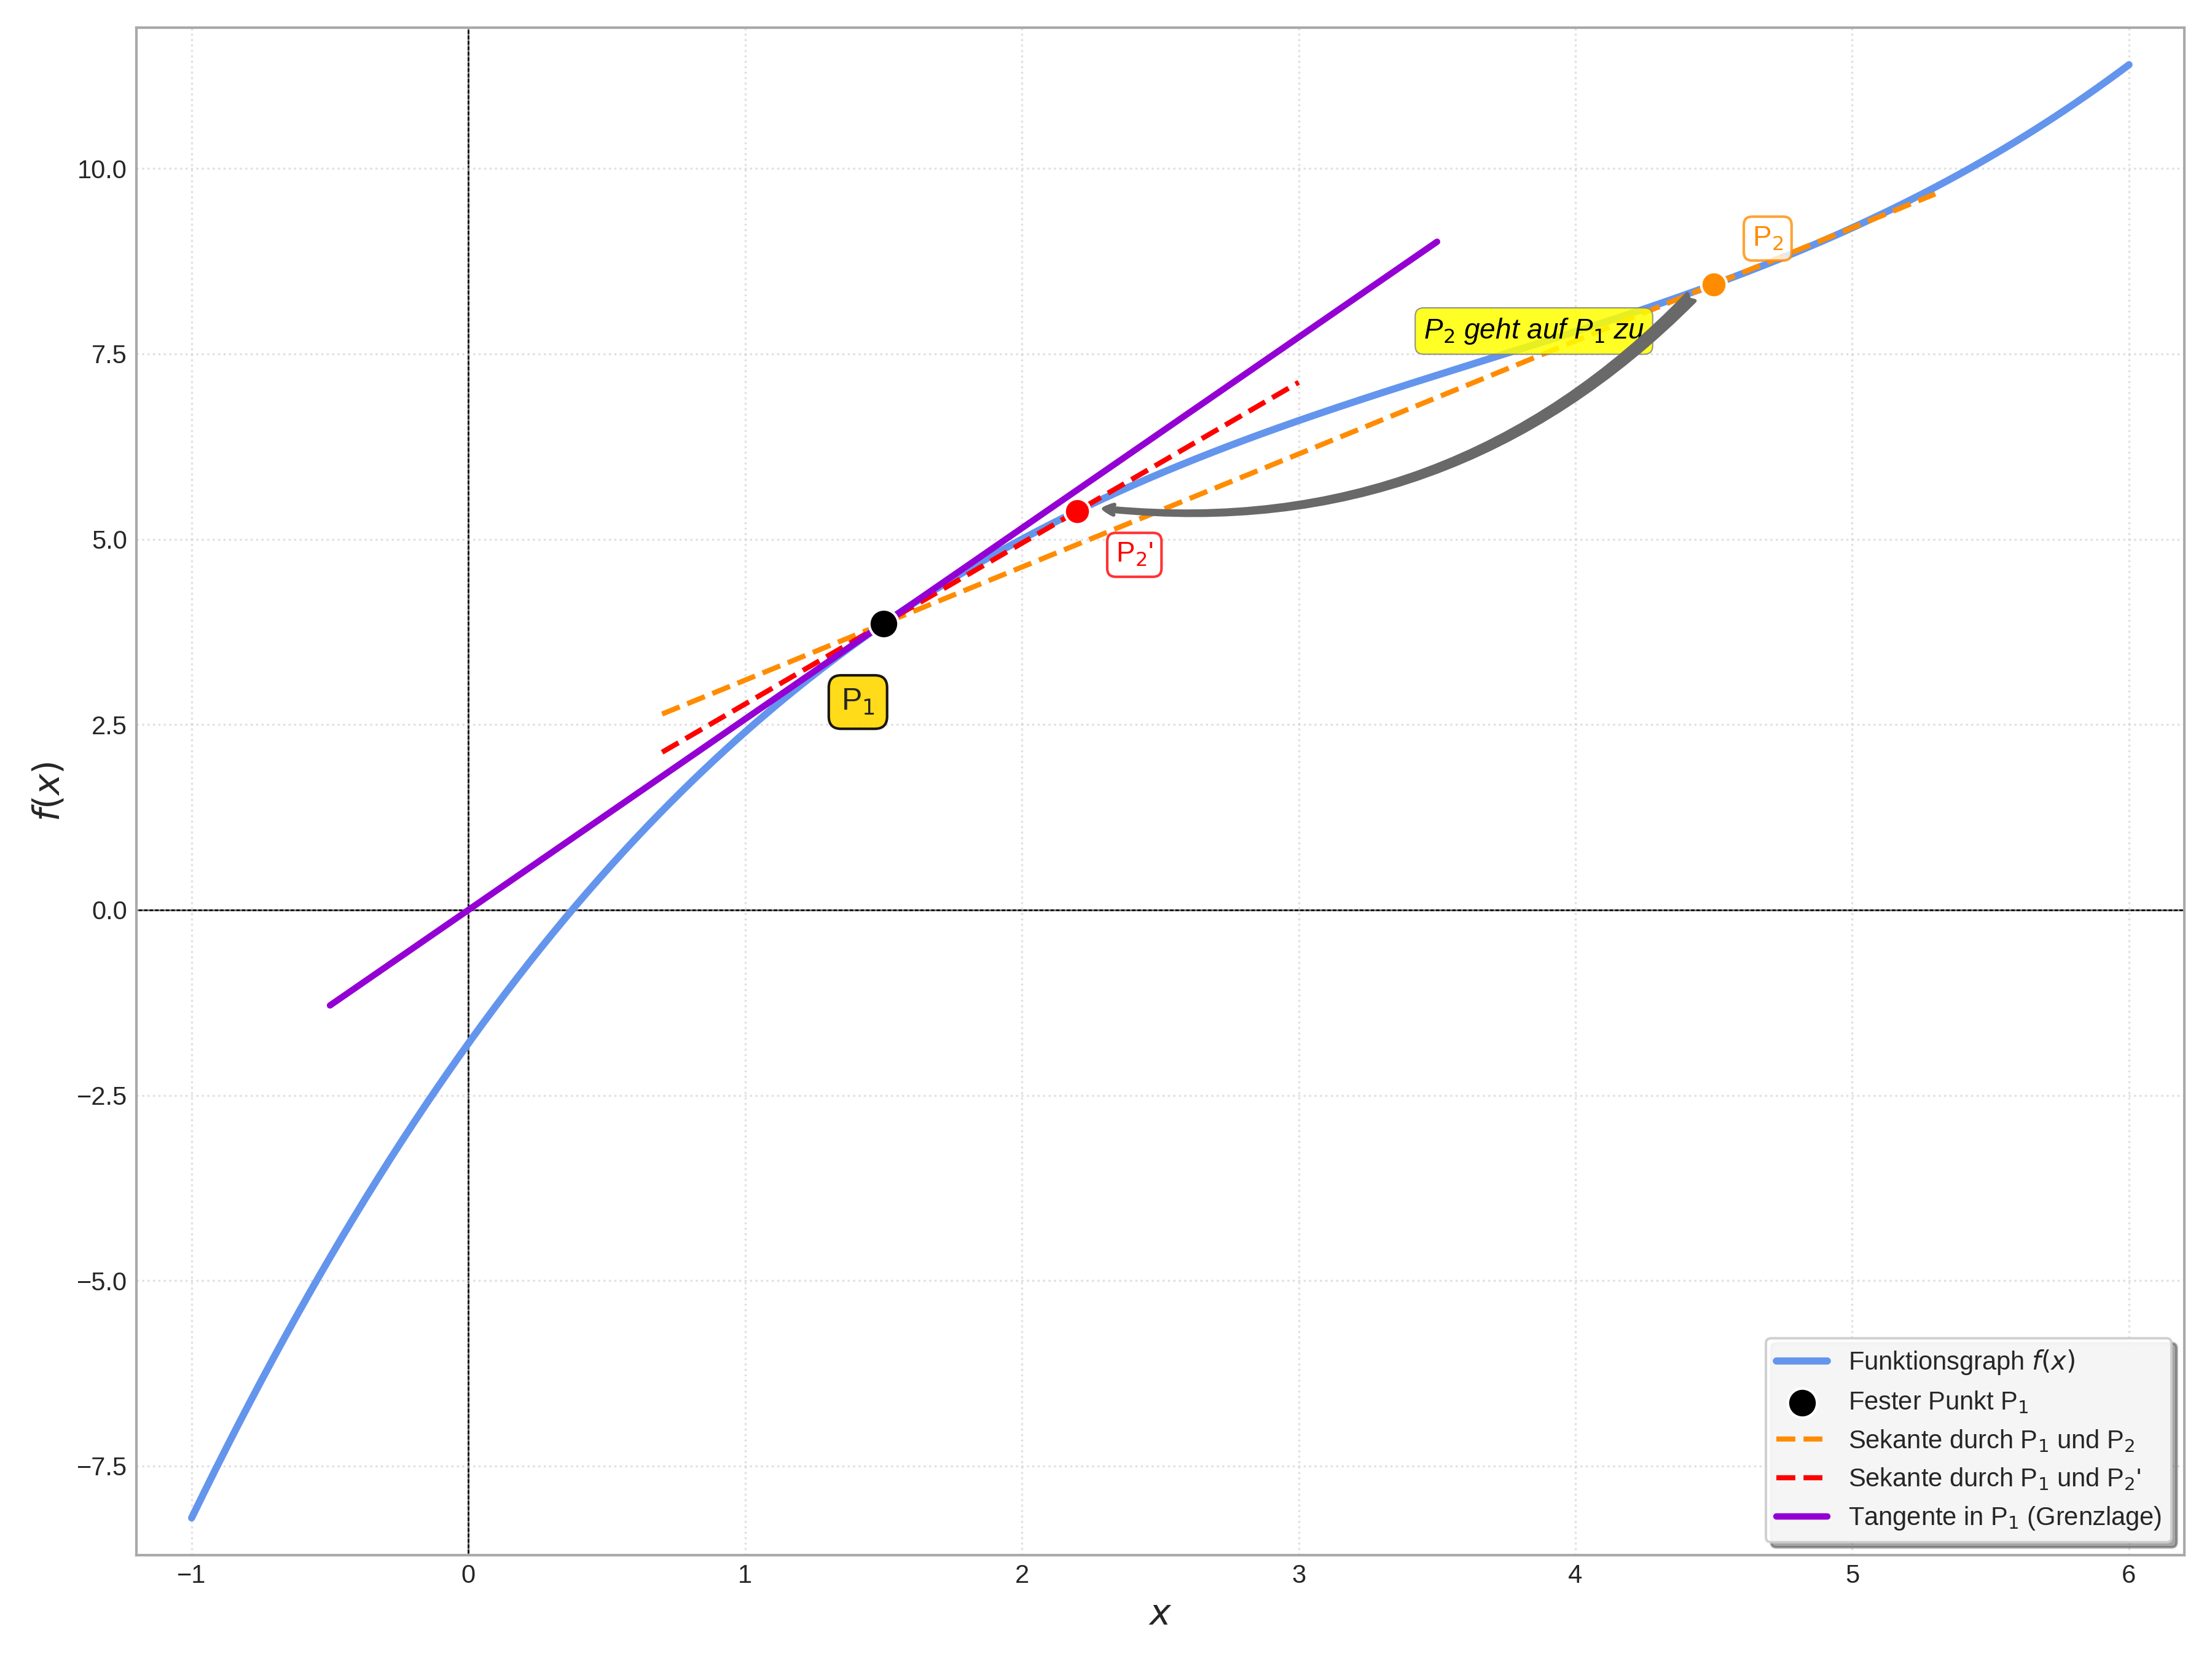
\includegraphics[scale=0.5]{grafiken/Differentialrechnung_Sekante_Tangente.png}
    \captionof{figure}{Von der Sekantensteigung zur Tangentensteigung}
    \label{fig:sek_zu_tan}
\end{center}
% Der Text geht hier direkt weiter

Dieser Prozess des 'Heranwanderns' wird mathematisch durch den \textbf{Grenzwert} (Limes) beschrieben. Die formale Definition der Ableitung lautet daher:
\[ f'(x_0) = \lim_{x \to x_0} \frac{f(x) - f(x_0)}{x - x_0}\, \text{ oder alternativ mit } h = x-x_0;  \, f'(x_0) = \lim_{h \to 0} \frac{f(x_0+h) - f(x_0)}{h} \]
Die zweite Form mit $h$ (die sogenannte \textbf{h-Methode}) ist oft praktischer für Berechnungen. Das Berechnen von Ableitungen über diesen Grenzwert kann aufwendig sein. Glücklicherweise gibt es für viele Funktionstypen feste Regeln, die uns das Ableiten erleichtern! Aber es ist wichtig, die Idee dahinter einmal verstanden zu haben.
\end{infoboxumgebung}

\begin{beispielumgebung}[Ableitung mit der h-Methode]{Ableitung von $f(x) = x^2 + 1$}
Wir wollen die Ableitung der Funktion $f(x) = x^2 + 1$ an einer beliebigen Stelle $x_0$ mit der h-Methode bestimmen.
Die Formel lautet: $f'(x_0) = \lim_{h \to 0} \frac{f(x_0+h) - f(x_0)}{h}$.

\textbf{Schritt 1: $f(x_0+h)$ und $f(x_0)$ bestimmen.}
$f(x_0) = x_0^2 + 1$
$f(x_0+h) = (x_0+h)^2 + 1 = (x_0^2 + 2x_0h + h^2) + 1 = x_0^2 + 2x_0h + h^2 + 1$.

\textbf{Schritt 2: Differenz $f(x_0+h) - f(x_0)$ bilden.}
$f(x_0+h) - f(x_0) = (x_0^2 + 2x_0h + h^2 + 1) - (x_0^2 + 1)$
$f(x_0+h) - f(x_0) = x_0^2 + 2x_0h + h^2 + 1 - x_0^2 - 1$
$f(x_0+h) - f(x_0) = 2x_0h + h^2$.

\textbf{Schritt 3: Differenzenquotient $\frac{f(x_0+h) - f(x_0)}{h}$ bilden und vereinfachen.}
$\frac{f(x_0+h) - f(x_0)}{h} = \frac{2x_0h + h^2}{h}$
Hier können wir $h$ aus dem Zähler ausklammern (solange $h \neq 0$, was für den Grenzwertprozess der Fall ist, da $h$ sich nur Null nähert):
$\frac{h(2x_0 + h)}{h} = 2x_0 + h$.

\textbf{Schritt 4: Grenzwert für $h \to 0$ bilden.}
$f'(x_0) = \lim_{h \to 0} (2x_0 + h)$.
Wenn $h$ gegen Null geht, wird der Term $2x_0+h$ zu $2x_0+0 = 2x_0$.
Also: $f'(x_0) = 2x_0$.

Da $x_0$ eine beliebige Stelle war, können wir auch schreiben: Die Ableitungsfunktion von $f(x)=x^2+1$ ist $f'(x)=2x$.
Das bedeutet, die Steigung der Tangente an die Parabel $y=x^2+1$ an der Stelle $x$ ist immer $2x$. An der Stelle $x=1$ ist die Steigung $2 \cdot 1 = 2$, an der Stelle $x=3$ ist sie $2 \cdot 3 = 6$.
\end{beispielumgebung}

\begin{aufgabenumgebung}{Experiment zur Sekantensteigung und h-Methode}
Gegeben ist die Funktion $f(x) = x^2$. Wir wollen die Steigung der Tangente im Punkt $P(1|1)$ untersuchen.
\begin{enumerate}
    \item \textbf{Experiment mit Sekantensteigungen:}
        Wähle einen festen Punkt $P_1(1|f(1))$. Berechne $f(1)$.
        Wähle nun verschiedene zweite Punkte $P_2(x|f(x))$, wobei $x$ immer näher an $1$ rückt. Berechne jeweils die Steigung der Sekante $m_{Sek} = \frac{f(x)-f(1)}{x-1}$.
        \begin{itemize}
            \item $x = 2$
            \item $x = 1.5$
            \item $x = 1.1$
            \item $x = 1.01$
            \item $x = 1.001$
        \end{itemize}
        Was beobachtest du bei den Werten für die Sekantensteigung? Welchem Wert scheinen sie sich anzunähern?
    \item \textbf{Exakte Berechnung mit der h-Methode:}
        Bestimme die Ableitung $f'(x_0)$ für $f(x)=x^2$ an der Stelle $x_0=1$ mit der h-Methode:
        $f'(1) = \lim_{h \to 0} \frac{f(1+h) - f(1)}{h}$.
        Vergleiche dein Ergebnis mit deiner Beobachtung aus Teil a).
    \item Bestimme die allgemeine Ableitungsfunktion $f'(x)$ für $f(x)=x^2$ mit der h-Methode.
\end{enumerate}
\end{aufgabenumgebung}

\begin{aufgabenumgebung}[h_methode_vertiefung]{Weitere Übungen zur h-Methode}
Bestimme die Ableitungsfunktion $f'(x)$ für die folgenden Funktionen mithilfe der h-Methode. Zeige alle algebraischen Umformungsschritte.
\begin{enumerate}
    \item $f(x) = 3x + 2$ 
        \begin{tippumgebung}{Lineare Funktion}
        Welche Steigung erwartest du bei einer linearen Funktion? Das Ergebnis der h-Methode sollte dies bestätigen.
        \end{tippumgebung}
    \item $f(x) = x^2 - x$
    \item $f(x) = c$ (wobei $c$ eine beliebige Konstante ist)
        \begin{tippumgebung}{Konstante Funktion}
        Wie sieht der Graph einer konstanten Funktion aus? Welche Steigung hat er überall?
        \end{tippumgebung}
    \item $f(x) = ax^2$ (wobei $a$ eine Konstante ist)
        \begin{tippumgebung}{Parameter $a$}
        Behandle $a$ während der Rechnung wie eine feste Zahl. Das Ergebnis wird $a$ enthalten.
        \end{tippumgebung}
\end{enumerate}
Diese Übungen helfen dir, das Prinzip der h-Methode zu verinnerlichen und algebraische Termumformungen zu trainieren.
\end{aufgabenumgebung}


\begin{erinnerungsboxumgebung}{Potenzgesetze – Fit im Umgang mit Exponenten}
Potenzen begegnen uns ständig, und ein sicherer Umgang mit den Potenzgesetzen ist Gold wert, nicht nur beim Ableiten! Hier eine Auffrischung der wichtigsten Regeln:

\paragraph{1. Grundlagen und Definitionen}
\begin{itemize}[nosep, leftmargin=2em]
    \item \textbf{Positive ganzzahlige Exponenten:} $a^n = \underbrace{a \cdot a \cdot \dots \cdot a}_{n \text{ Faktoren}}$ (für $n \in \mathbb{N}, n \ge 1$)
    \item \textbf{Exponent Null:} $a^0 = 1$ (für $a \neq 0$) \\ \textit{Beispiel:} $5^0 = 1$; $(-2)^0 = 1$
    \item \textbf{Exponent Eins:} $a^1 = a$ \\ \textit{Beispiel:} $x^1 = x$; $10^1 = 10$
\end{itemize}

\paragraph{2. Multiplikation und Division von Potenzen}
\begin{itemize}[nosep, leftmargin=2em]
    \item \textbf{Gleiche Basis, verschiedene Exponenten (Multiplikation):} $a^m \cdot a^n = a^{m+n}$ \\ \textit{Beispiel:} $x^3 \cdot x^2 = x^{3+2} = x^5$
    \item \textbf{Gleiche Basis, verschiedene Exponenten (Division):} $\frac{a^m}{a^n} = a^{m-n}$ (für $a \neq 0$) \\ \textit{Beispiel:} $\frac{x^7}{x^4} = x^{7-4} = x^3$
    \item \textbf{Gleicher Exponent, verschiedene Basen (Multiplikation):} $(a \cdot b)^n = a^n \cdot b^n$ \\ \textit{Beispiel:} $(2x)^3 = 2^3 \cdot x^3 = 8x^3$
    \item \textbf{Gleicher Exponent, verschiedene Basen (Division):} $\left(\frac{a}{b}\right)^n = \frac{a^n}{b^n}$ (für $b \neq 0$) \\ \textit{Beispiel:} $\left(\frac{x}{2}\right)^4 = \frac{x^4}{2^4} = \frac{x^4}{16}$
\end{itemize}

\paragraph{3. Potenzieren von Potenzen (Potenz einer Potenz)}
\begin{itemize}[nosep, leftmargin=2em]
    \item \textbf{Regel:} $(a^m)^n = a^{m \cdot n}$ \\ \textit{Beispiel:} $(x^3)^4 = x^{3 \cdot 4} = x^{12}$
\end{itemize}

\paragraph{4. Negative Exponenten}
Negative Exponenten bedeuten, dass die Potenz im Nenner eines Bruchs steht (oder umgekehrt).
\begin{itemize}[nosep, leftmargin=2em]
    \item \textbf{Definition:} $a^{-n} = \frac{1}{a^n}$ (für $a \neq 0$) \\ \textit{Beispiel:} $x^{-3} = \frac{1}{x^3}$; $2^{-4} = \frac{1}{2^4} = \frac{1}{16}$
    \item \textbf{Kehrwert eines Bruchs:} $\left(\frac{a}{b}\right)^{-n} = \left(\frac{b}{a}\right)^n = \frac{b^n}{a^n}$ (für $a,b \neq 0$) \\ \textit{Beispiel:} $\left(\frac{2}{5}\right)^{-2} = \left(\frac{5}{2}\right)^2 = \frac{5^2}{2^2} = \frac{25}{4}$
    \item \textbf{Im Nenner:} $\frac{1}{a^{-n}} = a^n$ (für $a \neq 0$) \\ \textit{Beispiel:} $\frac{1}{x^{-5}} = x^5$
\end{itemize}

\paragraph{5. Gebrochen rationale Exponenten (Wurzeln)}
Gebrochene Exponenten stehen für Wurzeln. Der Nenner des Exponenten ist der Wurzelexponent.
\begin{itemize}[nosep, leftmargin=2em]
    \item \textbf{Quadratwurzel:} $\sqrt{a} = a^{\frac{1}{2}}$ (für $a \ge 0$) \\ \textit{Beispiel:} $\sqrt{9} = 9^{\frac{1}{2}} = 3$
    \item \textbf{n-te Wurzel:} $\sqrt[n]{a} = a^{\frac{1}{n}}$ (für $a \ge 0$, wenn $n$ gerade ist) \\ \textit{Beispiel:} $\sqrt[3]{8} = 8^{\frac{1}{3}} = 2$; $\sqrt[4]{16} = 16^{\frac{1}{4}} = 2$
    \item \textbf{Allgemeiner gebrochener Exponent:} $a^{\frac{m}{n}} = \sqrt[n]{a^m} = (\sqrt[n]{a})^m$ \\ \textit{Beispiel:} $4^{\frac{3}{2}} = (\sqrt{4})^3 = 2^3 = 8$
    \textit{Beispiel mit negativem Bruch im Exponenten:} $8^{-\frac{2}{3}} = \frac{1}{8^{\frac{2}{3}}} = \frac{1}{(\sqrt[3]{8})^2} = \frac{1}{2^2} = \frac{1}{4}$
\end{itemize}

\vspace{0.5em}
\textbf{Kurze Übungen dazu:}
Vereinfache die folgenden Terme so weit wie möglich oder berechne den Wert:
\begin{multicols}{3}
\begin{enumerate}[label=(\alph*)]
    \item $x^5 \cdot x^{-3} = ?$
    \item $\frac{a^2}{a^6} = ?$
    \item $(y^4)^2 = ?$
    \item $(3b)^3 = ?$
    \item $\left(\frac{c}{4}\right)^2 = ?$
    \item $z^{-5} = ?$
    \item $\left(\frac{2}{x}\right)^{-3} = ?$
    \item $64^{\frac{1}{3}} = ?$
    \item $25^{\frac{3}{2}} = ?$
    \item $16^{-\frac{1}{4}} = ?$
    \item $\sqrt{x^8} = ?$
    \item $\frac{1}{y^{-2}} = ?$
    \item $(2x^2y^{-1})^3 = ?$
    \item $\frac{a^{\frac{1}{2}}}{a^{-\frac{1}{2}}} = ?$
    \item $(b^0 \cdot b^3)^{-1} = ?$
    \item $(x+2)^3 = ?$ \textit{(Tipp: Schreibe als $(x+2)^2 \cdot (x+2)$)}
\end{enumerate}
\end{multicols}
Diese Regeln sind sehr mächtig und helfen dir, auch komplizierte Terme zu zähmen!
\end{erinnerungsboxumgebung}


\begin{merksatzumgebung}[Ableitung – Das Wichtigste]{Was ist die Ableitung $f'(x)$?}
Die Ableitung $f'(x)$ einer Funktion $f(x)$ an einer Stelle $x$ (oft auch $x_0$ geschrieben) hat mehrere wichtige Bedeutungen:
\begin{itemize}
    \item Sie ist die \textbf{momentane Änderungsrate} der Funktion $f$ an der Stelle $x$.
    \item Sie ist die \textbf{Steigung der Tangente} an den Graphen von $f$ im Punkt $(x|f(x))$.
    \item Sie ist der \textbf{Grenzwert des Differenzenquotienten} (Steigung der Sekante), wenn das Intervall $\Delta x$ gegen Null geht.
\end{itemize}
Die Funktion $f'(x)$, die jeder Stelle $x$ ihre Ableitung zuordnet, heißt \textbf{Ableitungsfunktion} oder kurz Ableitung von $f$. Den Vorgang des Bestimmens der Ableitung nennt man \textbf{Differenzieren} oder \textbf{Ableiten}.
\end{merksatzumgebung}


\begin{warumwichtigumgebung}{Anwendungen der Ableitung}
Warum ist die Ableitung so ein mächtiges Werkzeug? Mit ihr können wir:
\begin{itemize}
    \item \textbf{Extremstellen} (Hoch- und Tiefpunkte) von Funktionen finden: Dort ist die Tangentensteigung (also die Ableitung) oft Null.
    \item Das \textbf{Monotonieverhalten} von Funktionen untersuchen: Wo steigt oder fällt ein Graph? (Positives Vorzeichen von $f'$ $\implies$ Graph steigt; negatives Vorzeichen von $f'$ $\implies$ Graph fällt).
    \item \textbf{Wendepunkte} finden: Punkte, an denen sich das Krümmungsverhalten eines Graphen ändert (z.B. von einer Rechts- in eine Linkskurve). Hier spielt die zweite Ableitung $f''(x)$ eine Rolle.
    \item \textbf{Optimierungsprobleme} lösen: Wo wird ein Wert maximal oder minimal (z.B. maximale Fläche, minimale Kosten)?
    \item \textbf{Physikalische Prozesse} beschreiben: Geschwindigkeit ist die Ableitung des Weges nach der Zeit, Beschleunigung ist die Ableitung der Geschwindigkeit nach der Zeit.
\end{itemize}
Die Differentialrechnung ist somit ein Schlüsselwerkzeug in vielen Naturwissenschaften, Ingenieurwissenschaften, Wirtschaftswissenschaften und natürlich in der Mathematik selbst.
\end{warumwichtigumgebung}

\begin{funfactbox}{Die Natur als schlaue Optimiererin}
Hast du dich jemals gefragt, warum Seifenblasen immer perfekt rund sind oder warum Bienen ihre Waben in exakten Sechsecken bauen? Es scheint, als ob die Natur eine eingebaute Mathematikerin ist, die ständig nach den besten, effizientesten Lösungen sucht!

\begin{itemize}
    \item \textbf{Seifenblasen:} Eine Seifenblase umschließt mit einer gegebenen Menge Seifenlösung ein maximales Volumen Luft. Die Kugelform ist dabei die geometrische Form, die bei gegebenem Volumen die kleinste Oberfläche hat. So minimiert die Seifenblase ihre Oberflächenspannung.
    \item \textbf{Bienenwaben:} Die sechseckige Struktur der Bienenwaben ist extrem stabil und materialsparend. Mit einer minimalen Menge Wachs wird maximaler Raum für Honig und Brut geschaffen.
    \item \textbf{Lichtstrahlen:} Licht nimmt immer den Weg der schnellsten Zeit (Fermatsches Prinzip). Daraus lassen sich die Gesetze der Reflexion und Brechung herleiten, die erklären, warum ein Strohhalm im Wasserglas geknickt aussieht.
\end{itemize}
Viele dieser 'optimalen' Formen und Wege in der Natur lassen sich mit den Werkzeugen der Differentialrechnung beschreiben und verstehen. Wenn wir zum Beispiel das Maximum oder Minimum einer Größe suchen (maximale Fläche, minimaler Materialverbrauch, schnellster Weg), suchen wir oft nach Stellen, an denen die Änderungsrate (also die Ableitung) Null wird. Es ist faszinierend, wie die Mathematik uns hilft, diese natürlichen 'Optimierungsstrategien' zu entschlüsseln!

\begin{center}
    
\includegraphics[width=0.6\textwidth]{grafiken/Natur_Optimierung.png}
    % Beschreibung für die Grafik 'Natur_Optimierung.png':
    % Die Grafik könnte eine kleine Collage zeigen: eine perfekte Seifenblase,
    % die sechseckige Struktur einer Bienenwabe und vielleicht einen Lichtstrahl,
    % der an einer Wasseroberfläche gebrochen wird (Brechungsgesetz).
    % Alternativ: Ein einzelnes starkes Bild, z.B. eine Nahaufnahme einer Schneeflocke (auch oft optimal geformt)
    % oder eine Sonnenblume mit ihren spiralförmig angeordneten Kernen.
    \captionof{figure}{Optimale Formen und Wege finden sich überall in der Natur.}
    \label{fig:natur_optimierung_funfact} % Eigenes Label für diese Grafik
\end{center}
\end{funfactbox}

\subsection{Ableitungsregeln – Dein Werkzeugkasten zum Differenzieren}

Glücklicherweise müssen wir nicht für jede Funktion mühsam den Grenzwert des Differenzenquotienten berechnen. Es gibt eine Reihe von \textbf{Ableitungsregeln}, die uns das Leben sehr erleichtern. Diese Regeln sind wie ein Werkzeugkasten – für jede Art von Funktion gibt es das passende Werkzeug. Wir werden diese Regeln Schritt für Schritt einführen und üben.

\subsubsection{Die Basis: Ableiten von Konstanten und Potenzen von $x$}

Fangen wir mit den grundlegendsten Bausteinen an.

\begin{merksatzumgebung}[Konstantenregel]{Ableitung einer konstanten Funktion}
Die Ableitung einer konstanten Funktion $f(x)=c$ (wobei $c$ eine beliebige reelle Zahl ist) ist immer Null.
\[ (c)' = 0 \]
\textbf{Beispiele:}
\begin{itemize}
    \item $f(x) = 5 \implies f'(x) = 0$
    \item $g(x) = -17.3 \implies g'(x) = 0$
    \item $h(x) = \pi \implies h'(x) = 0$ (denn $\pi$ ist auch nur eine Zahl/Konstante)
\end{itemize}
\textit{Warum ist das so?} Eine konstante Funktion hat einen waagerechten Graphen. Die Steigung einer waagerechten Geraden ist überall Null. Eine Konstante ändert sich nicht, ihre momentane Änderungsrate ist also Null.
\end{merksatzumgebung}

Die nächste wichtige Regel betrifft Potenzen von $x$.

\begin{merksatzumgebung}[Potenzregel]{Ableitung von $f(x) = x^n$}
Für Funktionen der Form $f(x) = x^n$ (wobei $n$ eine beliebige reelle Zahl sein kann, also auch Brüche oder negative Zahlen) ist die Ableitung:
\[ (x^n)' = n \cdot x^{n-1} \]
\textbf{Die Regel in Worten:} 'Ziehe den alten Exponenten als Faktor nach vorne und verringere dann den Exponenten um 1.'

\textbf{Beispiele:}
\begin{itemize}
    \item $f(x) = x^3 \implies n=3 \implies f'(x) = 3 \cdot x^{3-1} = 3x^2$
    \item $g(x) = x^7 \implies n=7 \implies g'(x) = 7 \cdot x^{7-1} = 7x^6$
    \item $h(x) = x = x^1 \implies n=1 \implies h'(x) = 1 \cdot x^{1-1} = 1 \cdot x^0 = 1 \cdot 1 = 1$
    (Die Ableitung von $f(x)=x$ ist also $1$. Das ist logisch, denn $y=x$ ist die Ursprungsgerade mit der Steigung 1.)
    \item $k(x) = \sqrt{x}$. Hier müssen wir erst umschreiben: $\sqrt{x} = x^{\frac{1}{2}}$. Also $n=\frac{1}{2}$.
    $k'(x) = \frac{1}{2} \cdot x^{\frac{1}{2}-1} = \frac{1}{2} \cdot x^{-\frac{1}{2}}$.
    Das kann man auch wieder umschreiben: $x^{-\frac{1}{2}} = \frac{1}{x^{\frac{1}{2}}} = \frac{1}{\sqrt{x}}$.
    Also: $k'(x) = \frac{1}{2\sqrt{x}}$.
    \item $m(x) = \frac{1}{x^2}$. Umschreiben: $\frac{1}{x^2} = x^{-2}$. Also $n=-2$.
    $m'(x) = -2 \cdot x^{-2-1} = -2 \cdot x^{-3}$.
    Umschreiben: $-2x^{-3} = -\frac{2}{x^3}$.
\end{itemize}
\end{merksatzumgebung}

\begin{tippumgebung}{Umgang mit Wurzeln und Brüchen beim Ableiten}
Um die Potenzregel auch für Wurzeln und Brüche mit $x$ im Nenner anwenden zu können, ist es sehr hilfreich, diese zuerst in Potenzschreibweise umzuwandeln:
\begin{itemize}
    \item $\sqrt[n]{x^m} = x^{\frac{m}{n}}$ (speziell: $\sqrt{x} = x^{\frac{1}{2}}$)
    \item $\frac{1}{x^k} = x^{-k}$ (speziell: $\frac{1}{x} = x^{-1}$)
\end{itemize}
Nach dem Ableiten kannst du das Ergebnis oft wieder in die ursprüngliche Schreibweise zurückführen, wenn das übersichtlicher ist.
\end{tippumgebung}

\subsubsection{Kombinationen: Faktor- und Summenregel}

Selten bestehen Funktionen nur aus einem einzigen $x^n$-Term. Meistens haben wir Vielfache davon oder Summen und Differenzen.

\begin{merksatzumgebung}[Faktorregel]{Ableitung von $c \cdot g(x)$}
Ein konstanter Faktor $c$ (also eine Zahl), der mit einer Funktion $g(x)$ multipliziert wird, bleibt beim Ableiten einfach erhalten und wird mit der Ableitung von $g(x)$ multipliziert:
\[ (c \cdot g(x))' = c \cdot g'(x) \]
\textbf{Beispiele:}
\begin{itemize}
    \item $f(x) = 5x^3$. Hier ist $c=5$ und $g(x)=x^3$. Wir wissen $(x^3)'=3x^2$.
    $f'(x) = 5 \cdot (x^3)' = 5 \cdot 3x^2 = 15x^2$.
    \item $g(x) = -2x^4 \implies g'(x) = -2 \cdot (x^4)' = -2 \cdot 4x^3 = -8x^3$.
    \item $h(x) = \frac{3}{x} = 3 \cdot \frac{1}{x} = 3 \cdot x^{-1}$.
    $h'(x) = 3 \cdot (x^{-1})' = 3 \cdot (-1x^{-2}) = -3x^{-2} = -\frac{3}{x^2}$.
\end{itemize}
\end{merksatzumgebung}

Die letzte Grundregel, die wir für Polynome brauchen, ist die Summenregel.

\begin{merksatzumgebung}[Summen- und Differenzregel]{Ableitung von $g(x) \pm h(x)$}
Die Ableitung einer Summe (oder Differenz) von zwei (oder mehr) Funktionen ist einfach die Summe (oder Differenz) ihrer einzelnen Ableitungen:
\[ (g(x) + h(x))' = g'(x) + h'(x) \]
\[ (g(x) - h(x))' = g'(x) - h'(x) \]
\textbf{In Worten:} 'Jeder Summand wird für sich abgeleitet, und die Ergebnisse werden dann addiert bzw. subtrahiert.'
\end{merksatzumgebung}

Mit diesen vier Regeln (Konstanten-, Potenz-, Faktor- und Summenregel) können wir nun jede beliebige ganzrationale Funktion (Polynomfunktion) ableiten!

\begin{beispielumgebung}[Ableiten einer Polynomfunktion]{Anwendung aller Grundregeln}
Leite die Funktion $f(x) = 4x^5 - \frac{2}{3}x^3 + 5x - \sqrt{2}$ ab.

Wir leiten jeden Summanden einzeln ab und nutzen dabei die Faktor- und Potenzregel:
\begin{itemize}
    \item $(4x^5)' = 4 \cdot (x^5)' = 4 \cdot (5x^4) = 20x^4$
    \item $(-\frac{2}{3}x^3)' = -\frac{2}{3} \cdot (x^3)' = -\frac{2}{3} \cdot (3x^2) = -2x^2$
    \item $(5x)' = 5 \cdot (x)' = 5 \cdot 1 = 5$
    \item $(-\sqrt{2})'$: Da $\sqrt{2}$ eine Konstante ist, ist ihre Ableitung $0$.
\end{itemize}
Zusammengesetzt ergibt das die Ableitungsfunktion:
\[ f'(x) = 20x^4 - 2x^2 + 5 \]
\end{beispielumgebung}

\begin{aufgabenumgebung}[A:EinfacheAbleitungen]{Grundregeln üben}
Leite die folgenden Funktionen ab. Notiere dir, welche Regeln du benutzt.
\begin{enumerate}
    \item $f_1(x) = 6x^4 - 3x^3 + 0.5x^2 - x + 12$
    \item $f_2(x) = -2x^5 + \frac{1}{4}x^4 - x^2 + 9x$
    \item $f_3(x) = (x-2)(x+3)$ (Tipp: Erst ausmultiplizieren!)
    \item $f_4(x) = 4\sqrt{x} - \frac{3}{x^2} + 2x^{-1}$ (Tipp: Erst in Potenzschreibweise umwandeln!)
    \item $f_5(x) = ax^2 + bx + c$ (Hier sind $a,b,c$ Konstanten/Parameter. Was ist die Ableitung?)
\end{enumerate}
\end{aufgabenumgebung}


\begin{tippumgebung}{Nach welcher Variable wird abgeleitet?}
In der Mathematik ist es üblich, dass Funktionen mit $f(x)$ bezeichnet werden und $x$ die Variable ist, nach der abgeleitet wird. Alle anderen Buchstaben in der Funktion (wie $a, b, c, k, \pi, \dots$) werden dann als \textbf{Konstanten} behandelt, es sei denn, es ist ausdrücklich etwas anderes gesagt (z.B. bei Funktionen mit mehreren Variablen, was aber erst viel später kommt).
Wenn eine Funktion z.B. $f(t) = at^2 + v_0t$ heißt, ist $t$ die Variable und $a$ sowie $v_0$ sind Konstanten. Die Ableitung nach $t$ wäre dann $f'(t) = 2at + v_0$.
Achte also immer genau darauf, welcher Buchstabe die Variable ist, nach der du ableiten sollst! Oft wird das durch die Schreibweise $f(x)$, $g(t)$, $A(r)$ etc. schon angedeutet.
Bei der h-Methode $f'(x_0) = \lim_{h \to 0} \frac{f(x_0+h) - f(x_0)}{h}$ ist $x_0$ der feste Punkt, an dem wir die Steigung suchen (wird also wie eine Konstante behandelt), und $h$ ist die Variable, die gegen Null geht. Die Ableitung $f'(x_0)$ ist dann die momentane Änderungsrate von $f$ bezüglich ihrer ursprünglichen Variablen (z.B. $x$), ausgewertet an der Stelle $x_0$.
\end{tippumgebung}

\begin{aufgabenumgebung}{Variable und Konstanten unterscheiden}
Leite die folgenden Funktionen nach der jeweils angegebenen Variablen ab. Behandle alle anderen Buchstaben als Konstanten.
\begin{enumerate}
    \item $f(t) = 5t^2 - at + b$. Leite nach $t$ ab. ($f'(t) = ?$)
    \item $g(a) = 3a^2x - 2at + 5x^2$. Leite nach $a$ ab. ($g'(a) = ?$)
    \item $s(t) = \frac{1}{2}gt^2 + v_0 t + s_0$. Leite nach $t$ ab. ($s'(t) = ?$) (Dies ist die Formel für den Weg bei gleichmäßiger Beschleunigung $g$ mit Anfangsgeschwindigkeit $v_0$ und Anfangsweg $s_0$.)
    \item $U(r) = 2\pi r$. Leite nach $r$ ab. ($U'(r) = ?$) (Umfang eines Kreises)
    \item $A(x) = k \cdot x^3 - m \cdot x$. Leite nach $x$ ab. ($A'(x) = ?$)
\end{enumerate}
\end{aufgabenumgebung}

\begin{warumwichtigumgebung}{Ableitung von Polynomen}
Das Ableiten von Polynomfunktionen ist eine fundamentale Fähigkeit. Viele komplexere Funktionen werden in der höheren Mathematik durch Polynome angenähert (z.B. durch Taylorreihen – ein Ausblick für später!). Wenn du Polynome sicher ableiten kannst, hast du eine wichtige Grundlage für viele weitere Themen der Analysis geschaffen, insbesondere für Kurvendiskussionen, bei denen Nullstellen der Ableitung (Extremstellen) und Nullstellen der zweiten Ableitung (Wendestellen) gesucht werden.
\end{warumwichtigumgebung}




\subsection{Die erste Ableitung $f'(x)$ – Was sie uns verrät}
\label{subsec:erste_ableitung_bedeutung}

Wir wissen jetzt, dass die erste Ableitung $f'(x)$ die Steigung der Tangente an den Graphen von $f(x)$ an der Stelle $x$ angibt. Aber was können wir daraus über den Verlauf der Funktion $f(x)$ schließen? Eine ganze Menge!

\subsubsection{Monotonie – Wo steigt und fällt der Graph?}

Das \textbf{Monotonieverhalten} einer Funktion beschreibt, in welchen Intervallen der Graph der Funktion steigt, fällt oder konstant verläuft. Die erste Ableitung ist hier unser Detektiv!

\begin{merksatzumgebung}{Monotonie und erste Ableitung}
Sei $f$ eine in einem Intervall $I$ differenzierbare Funktion. Dann gilt für alle $x \in I$:
\begin{itemize}
    \item Wenn $f'(x) > 0$ für alle $x$ in $I$, dann ist $f(x)$ in diesem Intervall \textbf{streng monoton steigend}. (Die Tangenten haben eine positive Steigung $\implies$ es geht bergauf).
    \item Wenn $f'(x) < 0$ für alle $x$ in $I$, dann ist $f(x)$ in diesem Intervall \textbf{streng monoton fallend}. (Die Tangenten haben eine negative Steigung $\implies$ es geht bergab).
    \item Wenn $f'(x) = 0$ für alle $x$ in $I$, dann ist $f(x)$ in diesem Intervall \textbf{konstant}. (Die Tangenten sind waagerecht).
\end{itemize}
Um die Monotonieintervalle einer Funktion zu bestimmen, untersuchst du also das \textbf{Vorzeichen der ersten Ableitung $f'(x)$}.
\end{merksatzumgebung}

\begin{beispielumgebung}{Monotonieverhalten untersuchen}
Untersuche das Monotonieverhalten der Funktion $f(x) = x^3 - 3x^2 + 1$.

\textbf{Schritt 1: Erste Ableitung bilden.}
$f'(x) = (x^3)' - (3x^2)' + (1)' = 3x^2 - 6x + 0 = 3x^2 - 6x$.

\textbf{Schritt 2: Nullstellen der ersten Ableitung finden.}
Wir setzen $f'(x) = 0$, um die Stellen zu finden, an denen die Tangente waagerecht ist (mögliche Extremstellen, an denen sich das Monotonieverhalten ändern könnte):
$3x^2 - 6x = 0$
Wir klammern $3x$ aus (Sonderfall $c=0$ bei quadratischen Gleichungen):
$3x(x - 2) = 0$
Die Lösungen sind $3x=0 \implies x_1 = 0$ und $x-2=0 \implies x_2 = 2$.
An den Stellen $x=0$ und $x=2$ hat die Funktion waagerechte Tangenten. Diese Stellen teilen die x-Achse in Intervalle, in denen wir das Vorzeichen von $f'(x)$ untersuchen.

\textbf{Schritt 3: Vorzeichen von $f'(x)$ in den Intervallen untersuchen.}
Die Nullstellen $x_1=0$ und $x_2=2$ teilen die x-Achse in drei offene Intervalle:
\begin{itemize}
    \item Intervall 1: $(-\infty, 0)$ (links von 0)
    \item Intervall 2: $(0, 2)$ (zwischen 0 und 2)
    \item Intervall 3: $(2, \infty)$ (rechts von 2)
\end{itemize}
Wir wählen für jedes Intervall einen Testwert und setzen ihn in $f'(x) = 3x^2 - 6x = 3x(x-2)$ ein:
\begin{itemize}
    \item Intervall 1: Wähle $x=-1$.
    $f'(-1) = 3(-1)^2 - 6(-1) = 3(1) + 6 = 3+6=9$.
    Da $f'(-1) = 9 > 0$, ist $f(x)$ im Intervall $(-\infty, 0)$ streng monoton steigend.
    
    \item Intervall 2: Wähle $x=1$.
    $f'(1) = 3(1)^2 - 6(1) = 3 - 6 = -3$.
    Da $f'(1) = -3 < 0$, ist $f(x)$ im Intervall $(0, 2)$ streng monoton fallend.

    \item Intervall 3: Wähle $x=3$.
    $f'(3) = 3(3)^2 - 6(3) = 3(9) - 18 = 27 - 18 = 9$.
    Da $f'(3) = 9 > 0$, ist $f(x)$ im Intervall $(2, \infty)$ streng monoton steigend.
\end{itemize}

\textbf{Zusammenfassung des Monotonieverhaltens:}
Basierend auf der Untersuchung der Vorzeichen von $f'(x)$ in den offenen Intervallen und der Tatsache, dass $f(x)$ als Polynomfunktion überall stetig ist, können wir schließen:
\begin{itemize}
    \item $f(x)$ ist \textbf{streng monoton steigend} für $x \in (-\infty, 0]$.
    \item $f(x)$ ist \textbf{streng monoton fallend} für $x \in [0, 2]$.
    \item $f(x)$ ist \textbf{streng monoton steigend} für $x \in [2, \infty)$.
\end{itemize}
\textit{Anmerkung zur Präzision:} Wenn wir sagen, eine Funktion ist 'streng monoton steigend auf $[a,b]$', bedeutet das, dass für alle $x_1, x_2 \in [a,b]$ mit $x_1 < x_2$ gilt $f(x_1) < f(x_2)$. Dies ist hier erfüllt, da $f'(x)$ in den \textit{offenen} Intervallen $(-\infty,0)$, $(0,2)$ und $(2,\infty)$ jeweils ein eindeutiges Vorzeichen hat und die Funktion $f$ an den Stellen $x=0$ und $x=2$ stetig ist. An den Punkten $x=0$ und $x=2$ selbst ist die Steigung $f'(x)$ zwar Null, die Funktion setzt aber ihren Trend (bis zu diesem Punkt steigend/fallend und ab diesem Punkt fallend/steigend) fort. Manchmal kann die Angabe von Monotonieintervallen mit offenen oder geschlossenen Klammern zu Diskussionen führen. Wichtig ist das Verständnis, dass sich das Monotonieverhalten \textit{an den Stellen ändern kann, wo $f'(x)=0$ ist}.


\begin{center}
    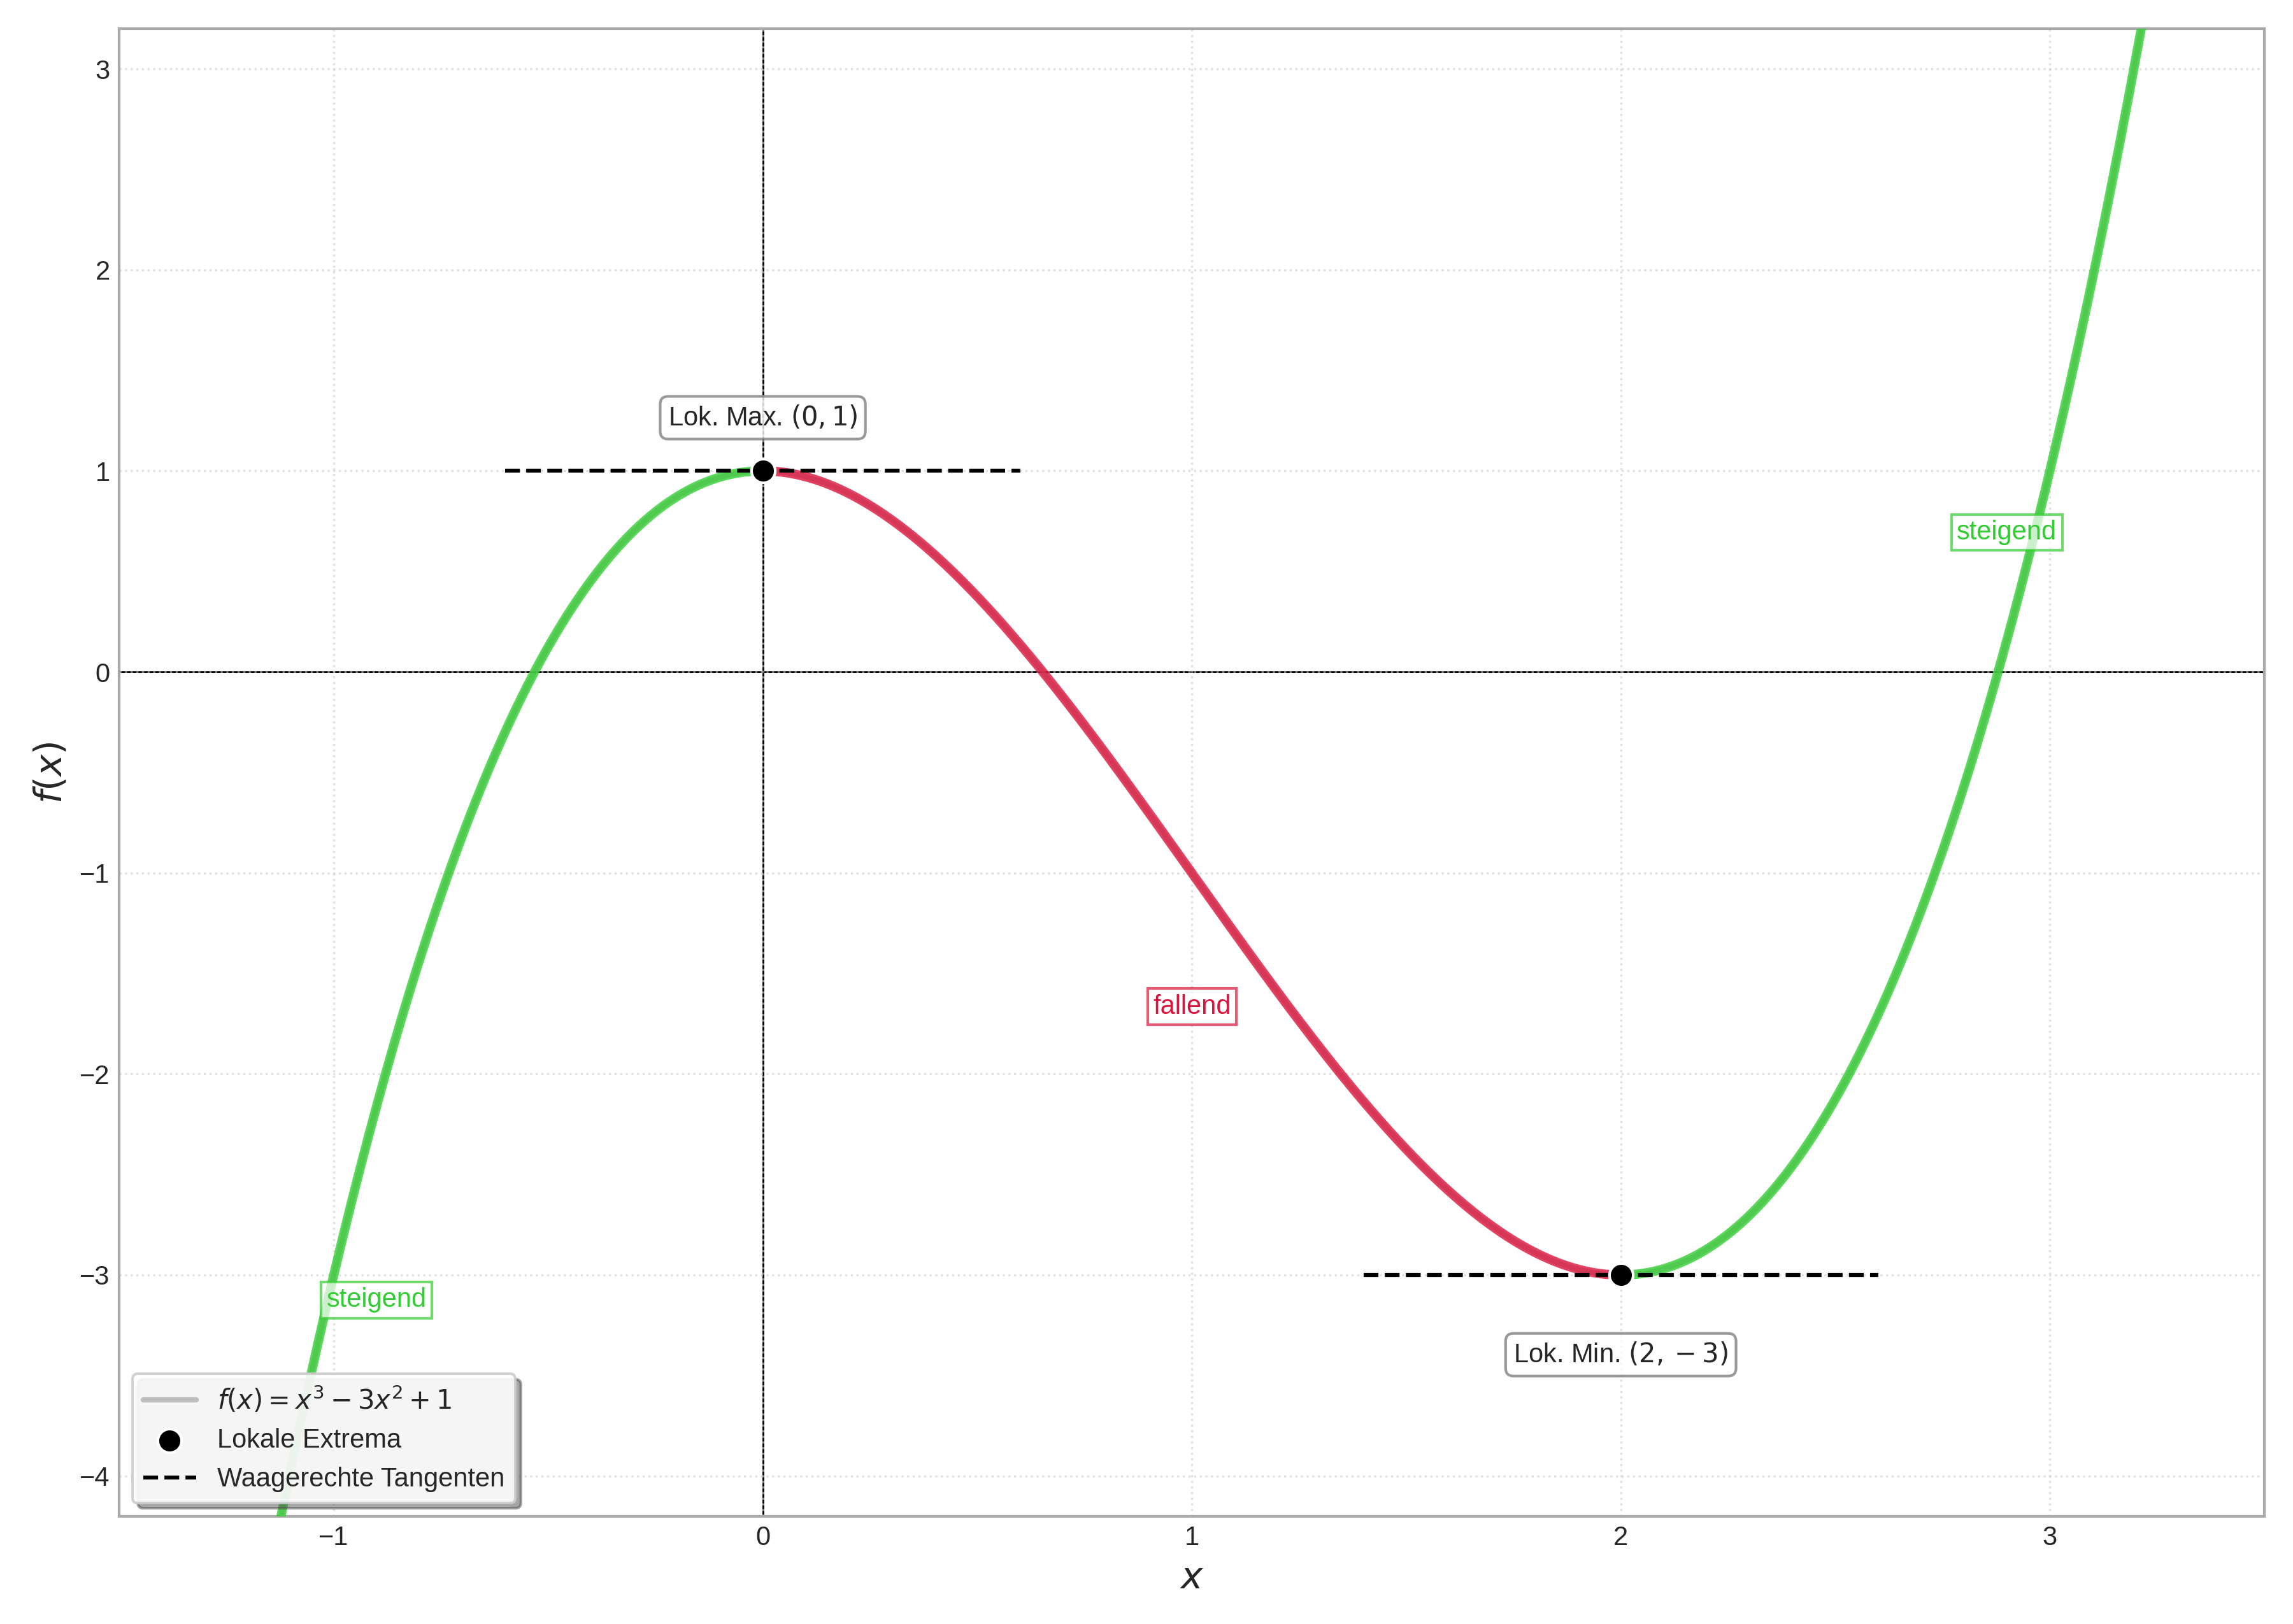
\includegraphics[width=0.8\textwidth]{grafiken/Monotonie_Polynom3Grades.png}
    \captionof{figure}{Monotonieverhalten von $f(x)=x^3-3x^2+1$}
    \label{fig:monotonie_bsp}
\end{center}
% Der Text geht hier direkt weiter

\end{beispielumgebung}

\begin{aufgabenumgebung}{Monotonie untersuchen – Vielfältige Polynome}
Untersuche das Monotonieverhalten der folgenden Funktionen. Bestimme dazu die erste Ableitung, deren Nullstellen und das Vorzeichen der Ableitung in den entsprechenden Intervallen. Skizziere grob den Verlauf der ersten Ableitung und überlege, was das für die Steigung der Originalfunktion bedeutet.
\begin{enumerate}
    \item $f_1(x) = x^3 - 6x^2 + 5$ 
        \begin{tippumgebung}{Nullstellen von $f_1'(x)$}
        Die Ableitung ist eine quadratische Funktion. Ihre Nullstellen kannst du mit der p-q-Formel oder Mitternachtsformel finden.
        \end{tippumgebung}
    \item $f_2(x) = \frac{1}{4}x^4 - x^3 + x^2$
        \begin{tippumgebung}{Nullstellen von $f_2'(x)$}
        Die Ableitung ist ein Polynom 3. Grades. Versuche, $x$ oder $x^2$ auszuklammern, um die Nullstellen zu finden.
        \end{tippumgebung}
    \item $f_3(x) = x^3 + 6x - 1$
        \begin{tippumgebung}{Immer positiv?}
        Untersuche die Ableitung $f_3'(x)$. Kann dieser Term jemals Null oder negativ werden? Was bedeutet das für die Monotonie von $f_3(x)$?
        \end{tippumgebung}
    \item $f_4(x) = -x^3 + 3x^2 - 3x + 2$
        \begin{tippumgebung}{Immer negativ?}
        Untersuche die Ableitung $f_4'(x)$. Kann dieser Term jemals Null oder positiv werden? (Hinweis: Quadratische Ergänzung bei $f_4'(x)$ könnte helfen, das Vorzeichen zu bestimmen.)
        \end{tippumgebung}
    \item $f_5(x) = x^3 - 4x^2 + 4x - 1$
        \begin{tippumgebung}{Nicht-ganzzahlige Nullstellen von $f_5'(x)$}
        Die Nullstellen der Ableitung sind hier nicht unbedingt ganze Zahlen, aber mit der Lösungsformel für quadratische Gleichungen gut zu finden.
        \end{tippumgebung}
    \item \textbf{Anwendung im Kontext:} Die Temperatur $T$ in Grad Celsius während eines bestimmten Tagesabschnitts kann näherungsweise durch die Funktion $T(t) = -0.1t^3 + 1.2t^2 - 2.5t + 15$ für $0 \le t \le 8$ (Stunden nach Beobachtungsbeginn) beschrieben werden. 
        \begin{itemize}
            \item In welchen Zeiträumen steigt die Temperatur?
            \item In welchen Zeiträumen fällt die Temperatur?
            \item Gibt es Zeitpunkte, an denen sich die Temperatur kurzzeitig nicht ändert (waagerechte Tangente)? Fällt an diesen Zeitpunkten etwas auf bezüglich der Temperatur? Versuche den Graph anhand der Monotonie und des y-Achsenabschnittes schon mal grob zu skizzieren! 
        \end{itemize}
\end{enumerate}
\end{aufgabenumgebung}

\subsubsection{Extremstellen – Gipfel und Täler im Funktionsgraphen}

Stellen, an denen die Funktion von steigend zu fallend übergeht (oder umgekehrt), sind oft besonders interessant. Hier liegen lokale \textbf{Hochpunkte} (Maxima) oder \textbf{Tiefpunkte} (Minima), zusammenfassend \textbf{Extrempunkte} genannt.

\begin{merksatzumgebung}{Extremstellen finden mit der ersten Ableitung}
Um lokale Extremstellen einer differenzierbaren Funktion $f(x)$ zu finden, gehst du wie folgt vor:

\textbf{1. Notwendige Bedingung für Extremstellen:}
Wenn $f(x)$ an der Stelle $x_E$ eine lokale Extremstelle hat, dann muss die Tangente dort waagerecht sein, also gilt:
\[ f'(x_E) = 0 \]
Die Stellen $x_E$, an denen $f'(x_E)=0$ ist, nennt man \textbf{kritische Stellen} oder \textbf{potentielle Extremstellen}. Nicht jede kritische Stelle ist aber automatisch eine Extremstelle (es könnte auch ein Sattelpunkt sein, dazu später mehr).

\textbf{2. Hinreichende Bedingung für Extremstellen (Vorzeichenwechselkriterium von $f'$):}
Nachdem du eine kritische Stelle $x_E$ (also eine Nullstelle von $f'(x)$) gefunden hast, musst du prüfen, ob dort tatsächlich ein Extremum vorliegt. Das geht mit dem Vorzeichenwechsel (VZW) von $f'(x)$ an der Stelle $x_E$:
\begin{itemize}
    \item Wenn $f'(x)$ an der Stelle $x_E$ das Vorzeichen von \textbf{Plus nach Minus} wechselt (d.h. $f(x)$ ist links von $x_E$ steigend und rechts davon fallend), dann hat $f(x)$ an der Stelle $x_E$ einen \textbf{lokalen Hochpunkt (Maximum)}.
    \item Wenn $f'(x)$ an der Stelle $x_E$ das Vorzeichen von \textbf{Minus nach Plus} wechselt (d.h. $f(x)$ ist links von $x_E$ fallend und rechts davon steigend), dann hat $f(x)$ an der Stelle $x_E$ einen \textbf{lokalen Tiefpunkt (Minimum)}.
    \item Wenn $f'(x)$ an der Stelle $x_E$ \textbf{keinen Vorzeichenwechsel} hat (z.B. von Plus nach Plus), dann liegt bei $x_E$ \textbf{kein Extrempunkt}, sondern ein Sattelpunkt (Terrassenpunkt) vor.
\end{itemize}
Die y-Koordinate des Extrempunktes erhältst du, indem du $x_E$ in die Originalfunktion $f(x)$ einsetzt: $y_E = f(x_E)$.
\end{merksatzumgebung}

\begin{tippumgebung}{Extrempunkte und Monotonie – Das Bild im Kopf}
\begin{itemize}
    \item \textbf{Hochpunkt (Maximum $\land$):} Der Graph steigt erst an ($f'(x)>0$, wie ein Pfeil $\nearrow$), erreicht den Gipfel (dort ist $f'(x_E)=0$), und fällt dann wieder ab ($f'(x)<0$, wie ein Pfeil $\searrow$). Die Form ähnelt einem 'Dach' oder einem umgedrehten 'V'.
    \item \textbf{Tiefpunkt (Minimum $\lor$):} Der Graph fällt erst ab ($f'(x)<0$, Pfeil $\searrow$), erreicht den Talboden ($f'(x_E)=0$), und steigt dann wieder an ($f'(x)>0$, Pfeil $\nearrow$). Die Form ähnelt einem 'Tal' oder einem 'V'.
\end{itemize}
Diese Vorstellung hilft dir, den Vorzeichenwechsel der ersten Ableitung richtig zu interpretieren. Später werden wir sehen, dass die zweite Ableitung $f''(x)$ uns eine alternative (und oft schnellere) Möglichkeit bietet, die Art eines Extrempunktes zu bestimmen, indem sie uns sagt, ob der Graph an dieser Stelle 'lachend' (linksgekrümmt $\implies$ Tiefpunkt) oder 'traurig' (rechtsgekrümmt $\implies$ Hochpunkt) ist.
\end{tippumgebung}

\begin{beispielumgebung}{Extremstellen bestimmen}
Bestimme die lokalen Extremstellen der Funktion $f(x) = x^3 - 3x^2 + 1$ aus dem vorherigen Beispiel.

Wir hatten bereits berechnet:
$f'(x) = 3x^2 - 6x$.
Die Nullstellen von $f'(x)$ waren $x_1=0$ und $x_2=2$. Das sind unsere kritischen Stellen.

Nun untersuchen wir den Vorzeichenwechsel von $f'(x)$ an diesen Stellen:
\begin{itemize}
    \item \textbf{Untersuchung bei $x_1=0$:}
        Wir wissen:
        Links von $x=0$ (z.B. bei $x=-1$) war $f'(-1)=9 > 0$ (steigend).
        Rechts von $x=0$ (z.B. bei $x=1$) war $f'(1)=-3 < 0$ (fallend).
        Es gibt also einen Vorzeichenwechsel von $f'(x)$ von $+$ nach $-$ bei $x=0$.
        Somit liegt bei $x=0$ ein \textbf{lokaler Hochpunkt} vor.
        Die y-Koordinate ist $f(0) = 0^3 - 3(0)^2 + 1 = 1$.
        Der Hochpunkt ist $H(0|1)$.

    \item \textbf{Untersuchung bei $x_2=2$:}
        Wir wissen:
        Links von $x=2$ (z.B. bei $x=1$) war $f'(1)=-3 < 0$ (fallend).
        Rechts von $x=2$ (z.B. bei $x=3$) war $f'(3)=9 > 0$ (steigend).
        Es gibt also einen Vorzeichenwechsel von $f'(x)$ von $-$ nach $+$ bei $x=2$.
        Somit liegt bei $x=2$ ein \textbf{lokaler Tiefpunkt} vor.
        Die y-Koordinate ist $f(2) = 2^3 - 3(2)^2 + 1 = 8 - 3(4) + 1 = 8 - 12 + 1 = -3$.
        Der Tiefpunkt ist $T(2|-3)$.
\end{itemize}
Die Funktion hat also einen Hochpunkt bei $H(0|1)$ und einen Tiefpunkt bei $T(2|-3)$.
\begin{center}
    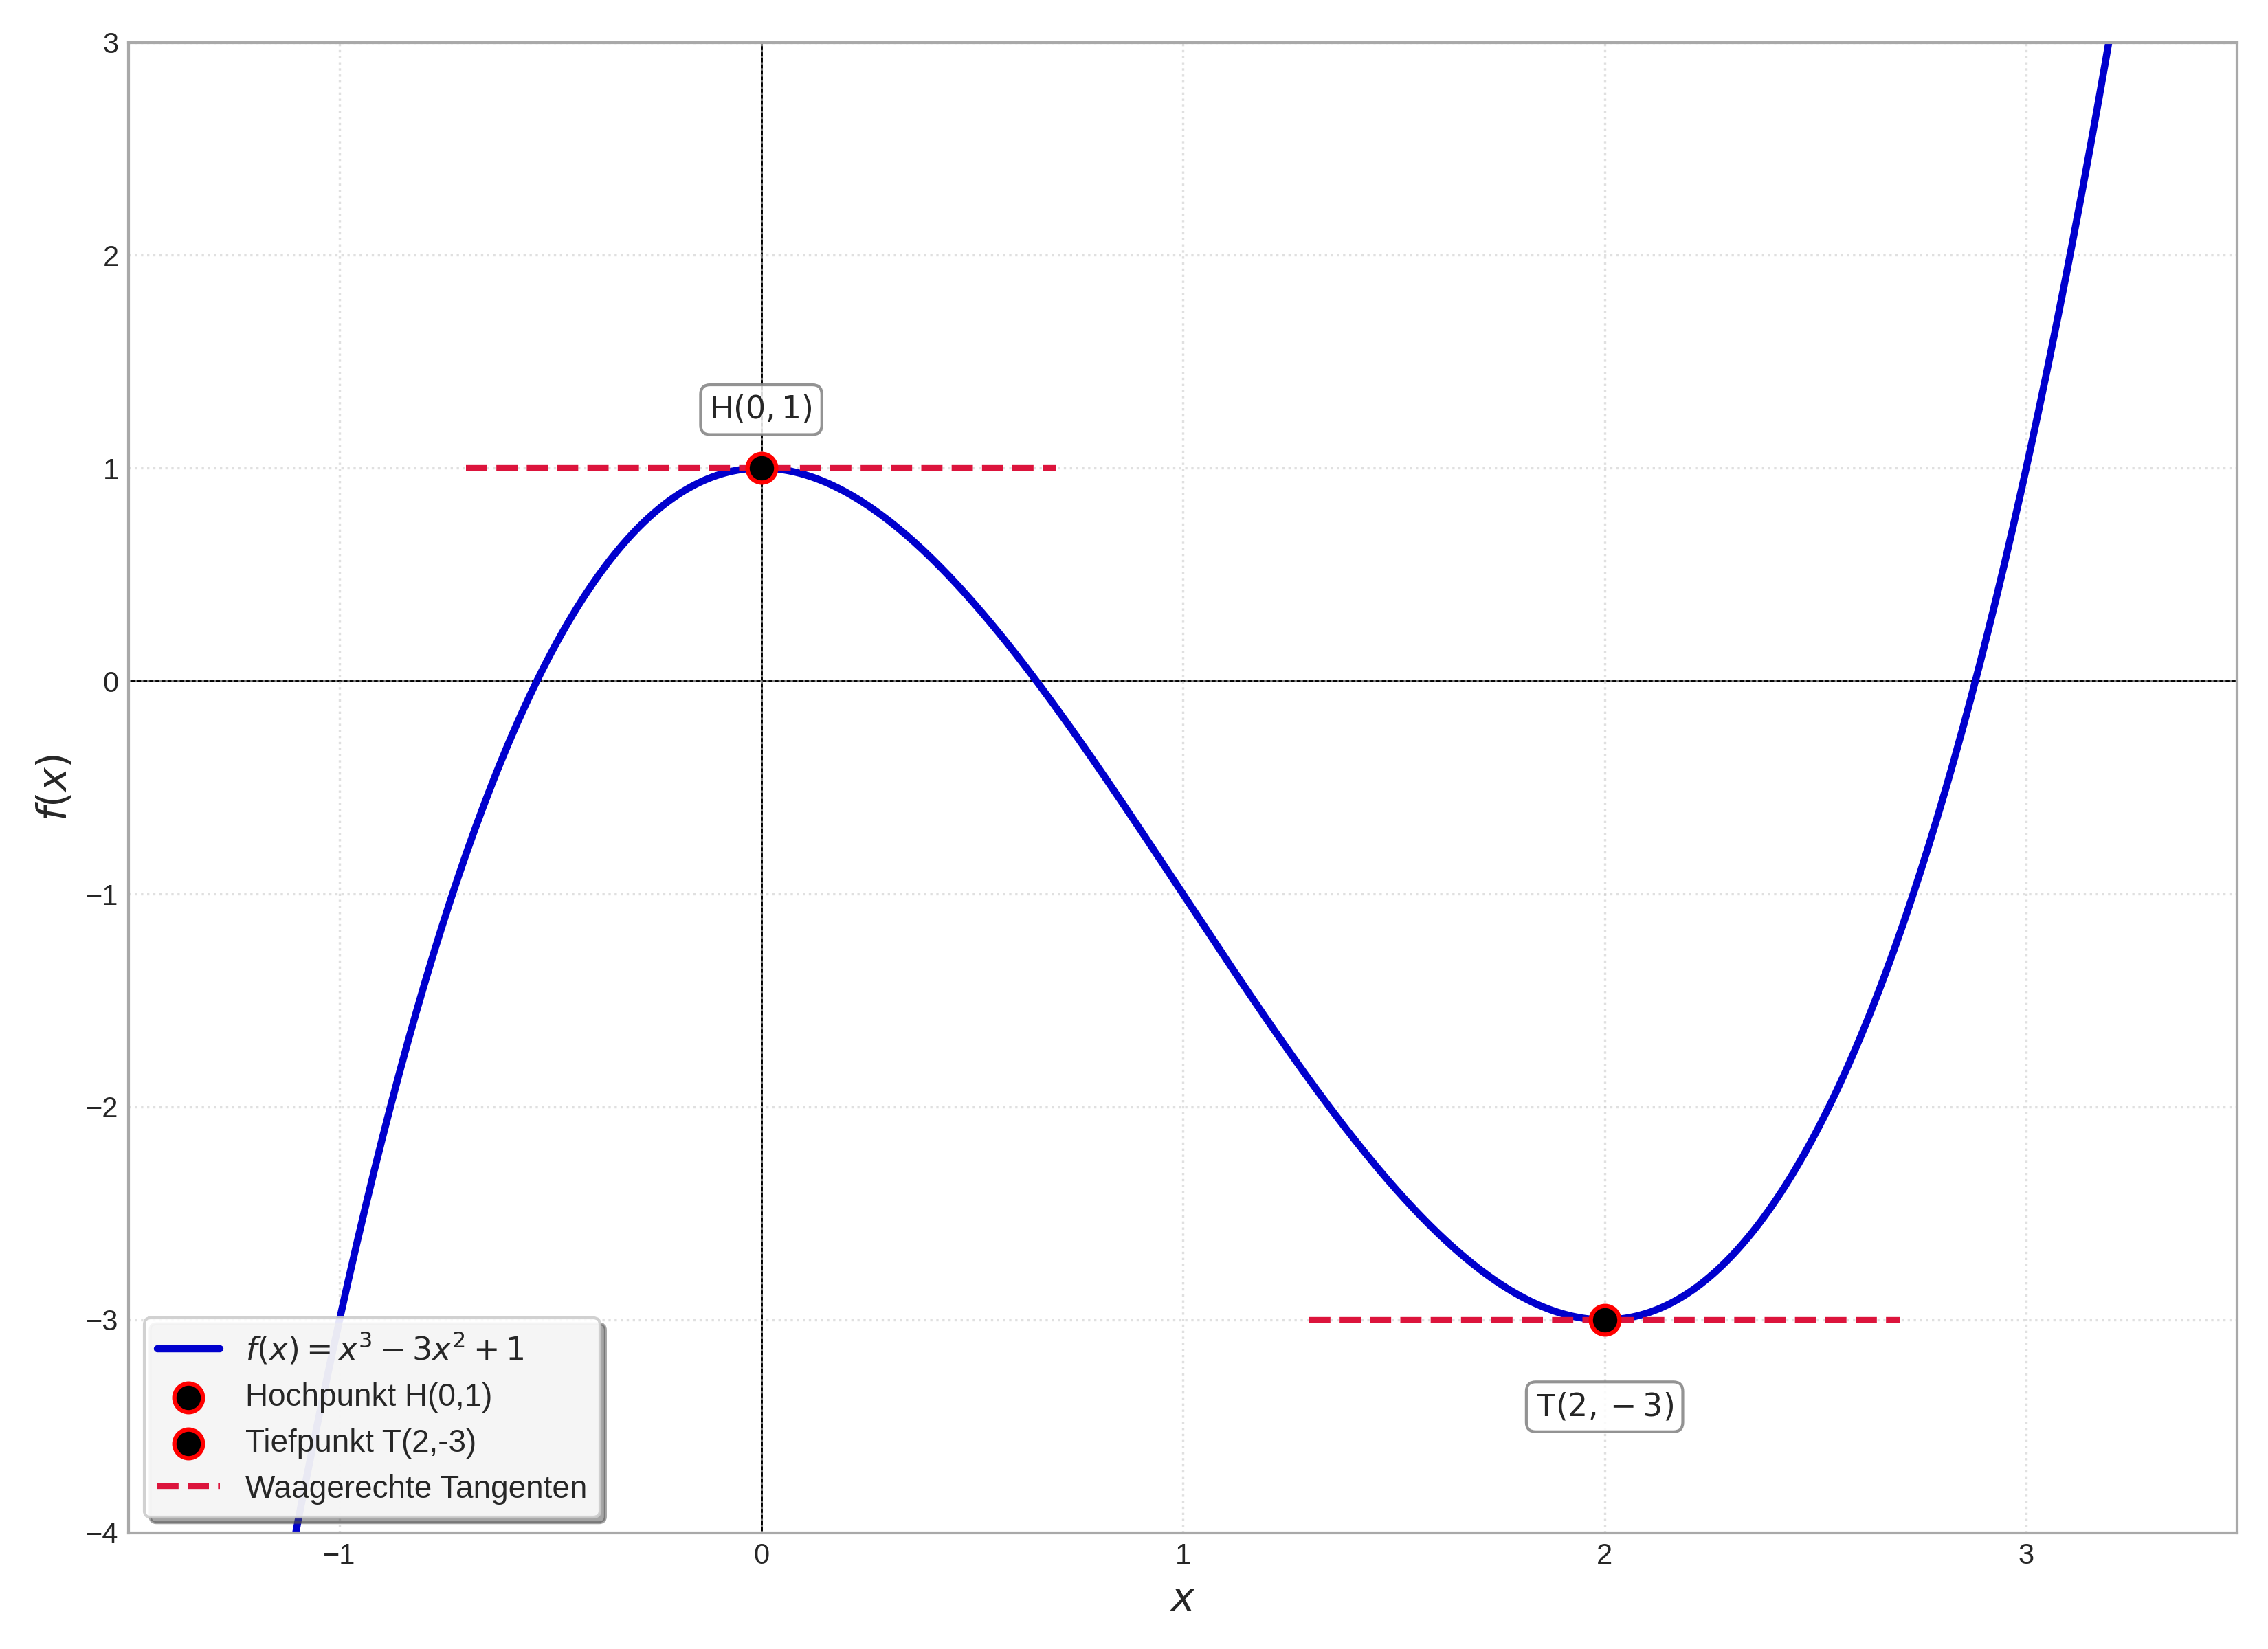
\includegraphics[width=0.8\textwidth]{grafiken/Differentialrechnung_Extrempunkte.png}
    \captionof{figure}{Hoch- und Tiefpunkt von $f(x)=x^3-3x^2+1$}
    \label{fig:extrempunkte_bsp}
\end{center}
\end{beispielumgebung}



% Dieser Block ersetzt den Inhalt der bestehenden 'aufgabenumgebung' 
% mit dem Titel 'Extrempunkte finden' im Kapitel 'Einführung in die Differentialrechnung',
% Unterabschnitt 'Extremstellen – Gipfel und Täler im Funktionsgraphen'.

\begin{aufgabenumgebung}{Extrempunkte finden – Vielfältige Herausforderungen}
Bestimme die lokalen Extrempunkte (Art und Koordinaten) der folgenden Funktionen. Verwende primär das \textbf{Vorzeichenwechselkriterium der ersten Ableitung ($f'(x)$)}. Du kannst deine Ergebnisse zusätzlich mit dem Kriterium der zweiten Ableitung ($f''(x)$) überprüfen, wo dies sinnvoll und einfach möglich ist.
\begin{enumerate}
    \item $f_1(x) = x^3 - 6x^2 + 9x + 1$
        \begin{tippumgebung}{Standardfall Polynom 3. Grades}
        Bestimme $f_1'(x)$. Finde die Nullstellen von $f_1'(x)$ (das sind deine Kandidaten für Extremstellen). Untersuche den Vorzeichenwechsel von $f_1'(x)$ an diesen Stellen, um die Art der Extrema (Hoch- oder Tiefpunkt) zu bestimmen. Zur Überprüfung kannst du auch $f_1''(x)$ bilden und die Kandidaten dort einsetzen. Vergiss nicht, auch die y-Koordinaten der Extrempunkte zu berechnen.
        \end{tippumgebung}

    \item $f_2(x) = \frac{1}{4}x^4 - x^3 - 2x^2 + 5$
        % \begin{tippumgebung}{Polynom 4. Grades}
        % Die erste Ableitung $f_2'(x)$ wird ein Polynom 3. Grades sein. Versuche, $x$ auszuklammern, um eine Nullstelle direkt zu finden. Die verbleibende quadratische Gleichung kannst du dann mit der p-q-Formel oder Mitternachtsformel lösen, um weitere Kandidaten für Extremstellen zu erhalten. Diese Funktion kann mehrere Extrempunkte haben.
        % \end{tippumgebung}

    \item $f_3(x) = x^4 - \frac{8}{3}x^3 + 2x^2$
        % \begin{tippumgebung}{Besonderer Fall bei $f_3''(x_E)=0$?}
        % Es kann vorkommen, dass für eine kritische Stelle $x_E$ (also $f_3'(x_E)=0$) auch die zweite Ableitung $f_3''(x_E)=0$ ist. In diesem Fall liefert das Kriterium mit der zweiten Ableitung keine Aussage über die Art des Extrempunkts. Dann musst du auf das Vorzeichenwechselkriterium der ersten Ableitung $f_3'(x)$ zurückgreifen, um zu entscheiden, ob ein Hochpunkt, Tiefpunkt oder vielleicht ein Sattelpunkt (kein Extremum) vorliegt.
        % \end{tippumgebung}

    \item \textbf{Schwer: Funktion mit Parameter $k$} \\
        Gegeben ist die Funktion $f_k(x) = x^3 - 3kx + 2$, wobei $k \in \mathbb{R}$ ein Parameter ist. Untersuche in Abhängigkeit von $k$:
        \begin{itemize}
            \item Für welche Werte von $k$ hat die Funktion $f_k(x)$ keine lokalen Extrempunkte?
            \item Für welche Werte von $k$ hat die Funktion $f_k(x)$ genau einen lokalen Extrempunkt? (Überlege, was das für die Ableitung bedeutet – kann ein Polynom 3. Grades nur einen Extrempunkt haben, wenn es nicht konstant ist?) Was liegt stattdessen an der kritischen Stelle vor, wenn es kein Extremum ist?
            \item Für welche Werte von $k$ hat die Funktion $f_k(x)$ genau zwei lokale Extrempunkte? Bestimme deren Art (Hoch-/Tiefpunkt) und ihre Lage (x-Koordinaten) in Abhängigkeit von $k$.
        \end{itemize}
        \begin{tippumgebung}{Fallunterscheidung für Parameter $k$}
        Die erste Ableitung ist $f_k'(x) = 3x^2 - 3k$. Setze $f_k'(x)=0$ und löse nach $x^2$. Die Anzahl der Lösungen für $x$ (und damit die Anzahl der kritischen Stellen) hängt vom Wert und Vorzeichen von $k$ ab. Unterscheide die Fälle $k<0$, $k=0$ und $k>0$. Nutze dann das Vorzeichenwechselkriterium von $f_k'(x)$ oder die zweite Ableitung $f_k''(x)$, um die Art der Extrema zu bestimmen.
        \end{tippumgebung}
    \item \textbf{Anwendung: Optimale Form}
        Ein oben offener quaderförmiger Behälter mit quadratischer Grundfläche soll ein Volumen von $V=32 \text{ cm}^3$ haben. Bestimme die Abmessungen (Seitenlänge der Grundfläche und Höhe), für die der Materialverbrauch (also die Oberfläche) minimal wird.
        \begin{enumerate}[label=(\alph*)]
            \item Sei $a$ die Seitenlänge der quadratischen Grundfläche und $h$ die Höhe des Quaders. Stelle die Formel für das Volumen $V$ und die Oberfläche $O$ (Grundfläche + 4 Seitenflächen) auf.
            \item Drücke $h$ mithilfe der Volumenformel durch $a$ aus (Nebenbedingung).
            \item Setze $h$ in die Oberflächenformel ein, um eine Zielfunktion $O(a)$ zu erhalten, die nur noch von $a$ abhängt.
            \item Bestimme die erste Ableitung $O'(a)$ und finde die kritischen Stellen.
            \item Überprüfe mit der zweiten Ableitung $O''(a)$, ob ein Minimum vorliegt. (Hier ist die zweite Ableitung oft der schnellste Weg zur Klassifizierung in Optimierungsaufgaben).
            \item Berechne die optimale Seitenlänge $a$ und die zugehörige Höhe $h$.
        \end{enumerate}
\end{enumerate}
\end{aufgabenumgebung}


\begin{tippumgebung}{Skizze hilft!}
Eine kleine Skizze des Vorzeichenverlaufs von $f'(x)$ (eine Art 'Zahlenstrahl' mit den Nullstellen von $f'$ und den Vorzeichen dazwischen) kann sehr helfen, um die Vorzeichenwechsel und damit die Art der Extrempunkte schnell zu erkennen. Es kann auch sehr helfen, alle bereits erlangten Kenntnisse über Funktionen auszunutzen, um $f'(x)$ zu skizzieren. Wenn die Nullstellen schon klar sind, dann kannst du schnell eine steigende/fallende lineare Funktion,welche durch den schnell ablesbaren y-Achsenabschnitt geht, skizzieren. Ähnliches gilt auch für Parabeln, du musst nur erkennen, ob die Parabel nach unten oder oben geöffnet ist.  
\end{tippumgebung}

\subsection{Höhere Ableitungen – Die Ableitung der Ableitung (und so weiter)}
\label{subsec:hoehere_ableitungen}

Wir haben gesehen, dass die erste Ableitung $f'(x)$ uns Informationen über die Steigung und das Monotonieverhalten der Funktion $f(x)$ gibt. Aber wir können auch die Ableitungsfunktion $f'(x)$ selbst wieder ableiten! Das Ergebnis nennen wir die \textbf{zweite Ableitung} von $f(x)$ und schreiben sie als $f''(x)$ (gelesen 'f zwei Strich von x').

\begin{merksatzumgebung}{Zweite und höhere Ableitungen}
\begin{itemize}
    \item Die \textbf{zweite Ableitung $f''(x)$} einer Funktion $f(x)$ ist die Ableitung ihrer ersten Ableitung $f'(x)$:
    \[ f''(x) = (f'(x))' \]
    \item Man kann diesen Prozess fortsetzen: Die Ableitung der zweiten Ableitung ist die \textbf{dritte Ableitung $f'''(x)$}, die Ableitung der dritten ist die \textbf{vierte Ableitung $f^{(4)}(x)$} (ab hier verwendet man oft römische Ziffern oder Zahlen in Klammern, um die Striche zu vermeiden), und so weiter.
    \[ f'''(x) = (f''(x))' \]
    \[ f^{(n)}(x) = (f^{(n-1)}(x))' \quad (\text{die n-te Ableitung}) \]
\end{itemize}
\end{merksatzumgebung}

\begin{warumwichtigumgebung}{Bedeutung höherer Ableitungen}
\begin{itemize}
    \item \textbf{Erste Ableitung $f'(x)$:} Gibt die Steigung von $f(x)$ an. In der Physik: Wenn $s(t)$ der Weg ist, ist $s'(t)$ die Geschwindigkeit $v(t)$.
    \item \textbf{Zweite Ableitung $f''(x)$:} Gibt die \textit{Änderung der Steigung} von $f(x)$ an. Sie beschreibt das \textbf{Krümmungsverhalten} des Graphen von $f(x)$. In der Physik: Wenn $v(t)$ die Geschwindigkeit ist, ist $v'(t) = s''(t)$ die Beschleunigung $a(t)$. Die zweite Ableitung sagt uns also, wie schnell sich die Geschwindigkeit ändert.
    \item \textbf{Dritte Ableitung $f'''(x)$ und höher:} Haben auch ihre Bedeutungen, z.B. in der Physik der 'Ruck' (Änderung der Beschleunigung), sind aber in der Schulmathematik für Kurvendiskussionen seltener direkt relevant als $f'$ und $f''$.
\end{itemize}
Die zweite Ableitung ist also die 'Ableitung der Steigung' oder die 'Steigung der Steigungsfunktion'.
\end{warumwichtigumgebung}

\begin{beispielumgebung}{Höhere Ableitungen bilden}
Bestimme die ersten drei Ableitungen der Funktion $f(x) = x^4 - 5x^3 + 2x^2 - 7x + 10$.

$f(x) = x^4 - 5x^3 + 2x^2 - 7x + 10$

$f'(x) = (x^4)' - (5x^3)' + (2x^2)' - (7x)' + (10)'$
$f'(x) = 4x^3 - 5 \cdot 3x^2 + 2 \cdot 2x - 7 \cdot 1 + 0$
$f'(x) = 4x^3 - 15x^2 + 4x - 7$

$f''(x) = (f'(x))' = (4x^3 - 15x^2 + 4x - 7)'$
$f''(x) = (4x^3)' - (15x^2)' + (4x)' - (7)'$
$f''(x) = 4 \cdot 3x^2 - 15 \cdot 2x + 4 \cdot 1 - 0$
$f''(x) = 12x^2 - 30x + 4$

$f'''(x) = (f''(x))' = (12x^2 - 30x + 4)'$
$f'''(x) = (12x^2)' - (30x)' + (4)'$
$f'''(x) = 12 \cdot 2x - 30 \cdot 1 + 0$
$f'''(x) = 24x - 30$

Man könnte so weitermachen: $f^{(4)}(x) = 24$, $f^{(5)}(x) = 0$, und alle weiteren Ableitungen wären ebenfalls null.
\end{beispielumgebung}

\begin{aufgabenumgebung}{Höhere Ableitungen berechnen}
Bestimme die erste, zweite und dritte Ableitung der folgenden Funktionen:
\begin{enumerate}
    \item $f(x) = 2x^3 - 9x^2 + 12x - 5$
    \item $g(x) = -0.1x^5 + x^3 - 7$
    \item $h(t) = 2t^2 - \frac{1}{t}$ (Tipp: $\frac{1}{t} = t^{-1}$)
\end{enumerate}
\end{aufgabenumgebung}

\subsection{Die zweite Ableitung $f''(x)$ – Krümmung und Wendepunkte}
\label{subsec:zweite_ableitung_neu} 

Nachdem wir wissen, was höhere Ableitungen sind, konzentrieren wir uns nun auf die Bedeutung der \textbf{zweiten Ableitung $f''(x)$}. Sie gibt uns Auskunft über das \textbf{Krümmungsverhalten} des Graphen von $f(x)$ und hilft uns, \textbf{Wendepunkte} zu finden.

\subsubsection{Krümmungsverhalten – Links- oder Rechtskurve?}
Die zweite Ableitung beschreibt, wie sich die Steigung der Funktion ändert.
\begin{itemize}
    \item Wenn $f''(x) > 0$, bedeutet das, dass die Steigung $f'(x)$ zunimmt. Stell dir vor, du fährst auf dem Graphen: Erst ist die Steigung vielleicht negativ (bergab), dann wird sie weniger negativ, dann Null, dann positiv (bergauf). Das entspricht einer \textbf{Linkskurve} (man sagt auch, der Graph ist \textbf{konvex} oder 'nach oben offen' in diesem Bereich).
    \item Wenn $f''(x) < 0$, bedeutet das, dass die Steigung $f'(x)$ abnimmt. Du fährst vielleicht erst steil bergauf, dann wird der Anstieg flacher, dann Null, dann geht es bergab. Das entspricht einer \textbf{Rechtskurve} (man sagt auch, der Graph ist \textbf{konkav} oder 'nach unten offen' in diesem Bereich).
\end{itemize}

\begin{merksatzumgebung}{Krümmung und zweite Ableitung}
Sei $f$ eine in einem Intervall $I$ zweimal differenzierbare Funktion. Dann gilt für alle $x \in I$:
\begin{itemize}
    \item Wenn $f''(x) > 0$ für alle $x$ in $I$, dann ist der Graph von $f(x)$ in diesem Intervall \textbf{linksgekrümmt} (konvex). (Der Graph macht eine 'Linkskurve', wie ein lachender Smiley $\smile$ bei positiver zweiten Ableitung).
    \item Wenn $f''(x) < 0$ für alle $x$ in $I$, dann ist der Graph von $f(x)$ in diesem Intervall \textbf{rechtsgekrümmt} (konkav). (Der Graph macht eine 'Rechtskurve', wie ein trauriger Smiley $\frown$ bei negativer zweiten Ableitung).
    \item Wenn $f''(x) = 0$ an einer Stelle $x_W$, dann \textbf{könnte} dort ein \textbf{Wendepunkt} vorliegen (ein Punkt, an dem sich das Krümmungsverhalten ändert).
\end{itemize}
Um die Krümmungsintervalle zu bestimmen, untersuchst du also das \textbf{Vorzeichen der zweiten Ableitung $f''(x)$}.
\end{merksatzumgebung}

\begin{beispielumgebung}{Krümmungsverhalten untersuchen}
Untersuche das Krümmungsverhalten von $f(x) = x^3 - 3x^2 + 1$.
Wir hatten $f'(x) = 3x^2 - 6x$ und $f''(x) = 6x - 6$.

\textbf{Schritt 1: Nullstellen der zweiten Ableitung finden.}
$f''(x) = 0 \implies 6x - 6 = 0$
\begin{center}
\begin{tabular}{r @{\,} c @{\,} l @{\quad\quad} l}
$6x - 6$ & $=$ & $0$ & $|+6$ \\
$6x$ & $=$ & $6$ & $|:6$ \\
$x$ & $=$ & $1$ & \\
\end{tabular}
\end{center}
An der Stelle $x=1$ könnte sich das Krümmungsverhalten ändern.

\textbf{Schritt 2: Vorzeichen von $f''(x)$ in den Intervallen untersuchen.}
Die Stelle $x=1$ teilt die x-Achse in zwei Intervalle: $(-\infty, 1)$ und $(1, \infty)$.
\begin{itemize}
    \item Intervall $(-\infty, 1)$: Wähle Testwert $x=0$. $f''(0) = 6(0) - 6 = -6$.
    Da $f''(0) < 0$, ist der Graph von $f(x)$ im Intervall $(-\infty, 1)$ rechtsgekrümmt.
    \item Intervall $(1, \infty)$: Wähle Testwert $x=2$. $f''(2) = 6(2) - 6 = 12 - 6 = 6$.
    Da $f''(2) > 0$, ist der Graph von $f(x)$ im Intervall $(1, \infty)$ linksgekrümmt.
\end{itemize}
\begin{center}
    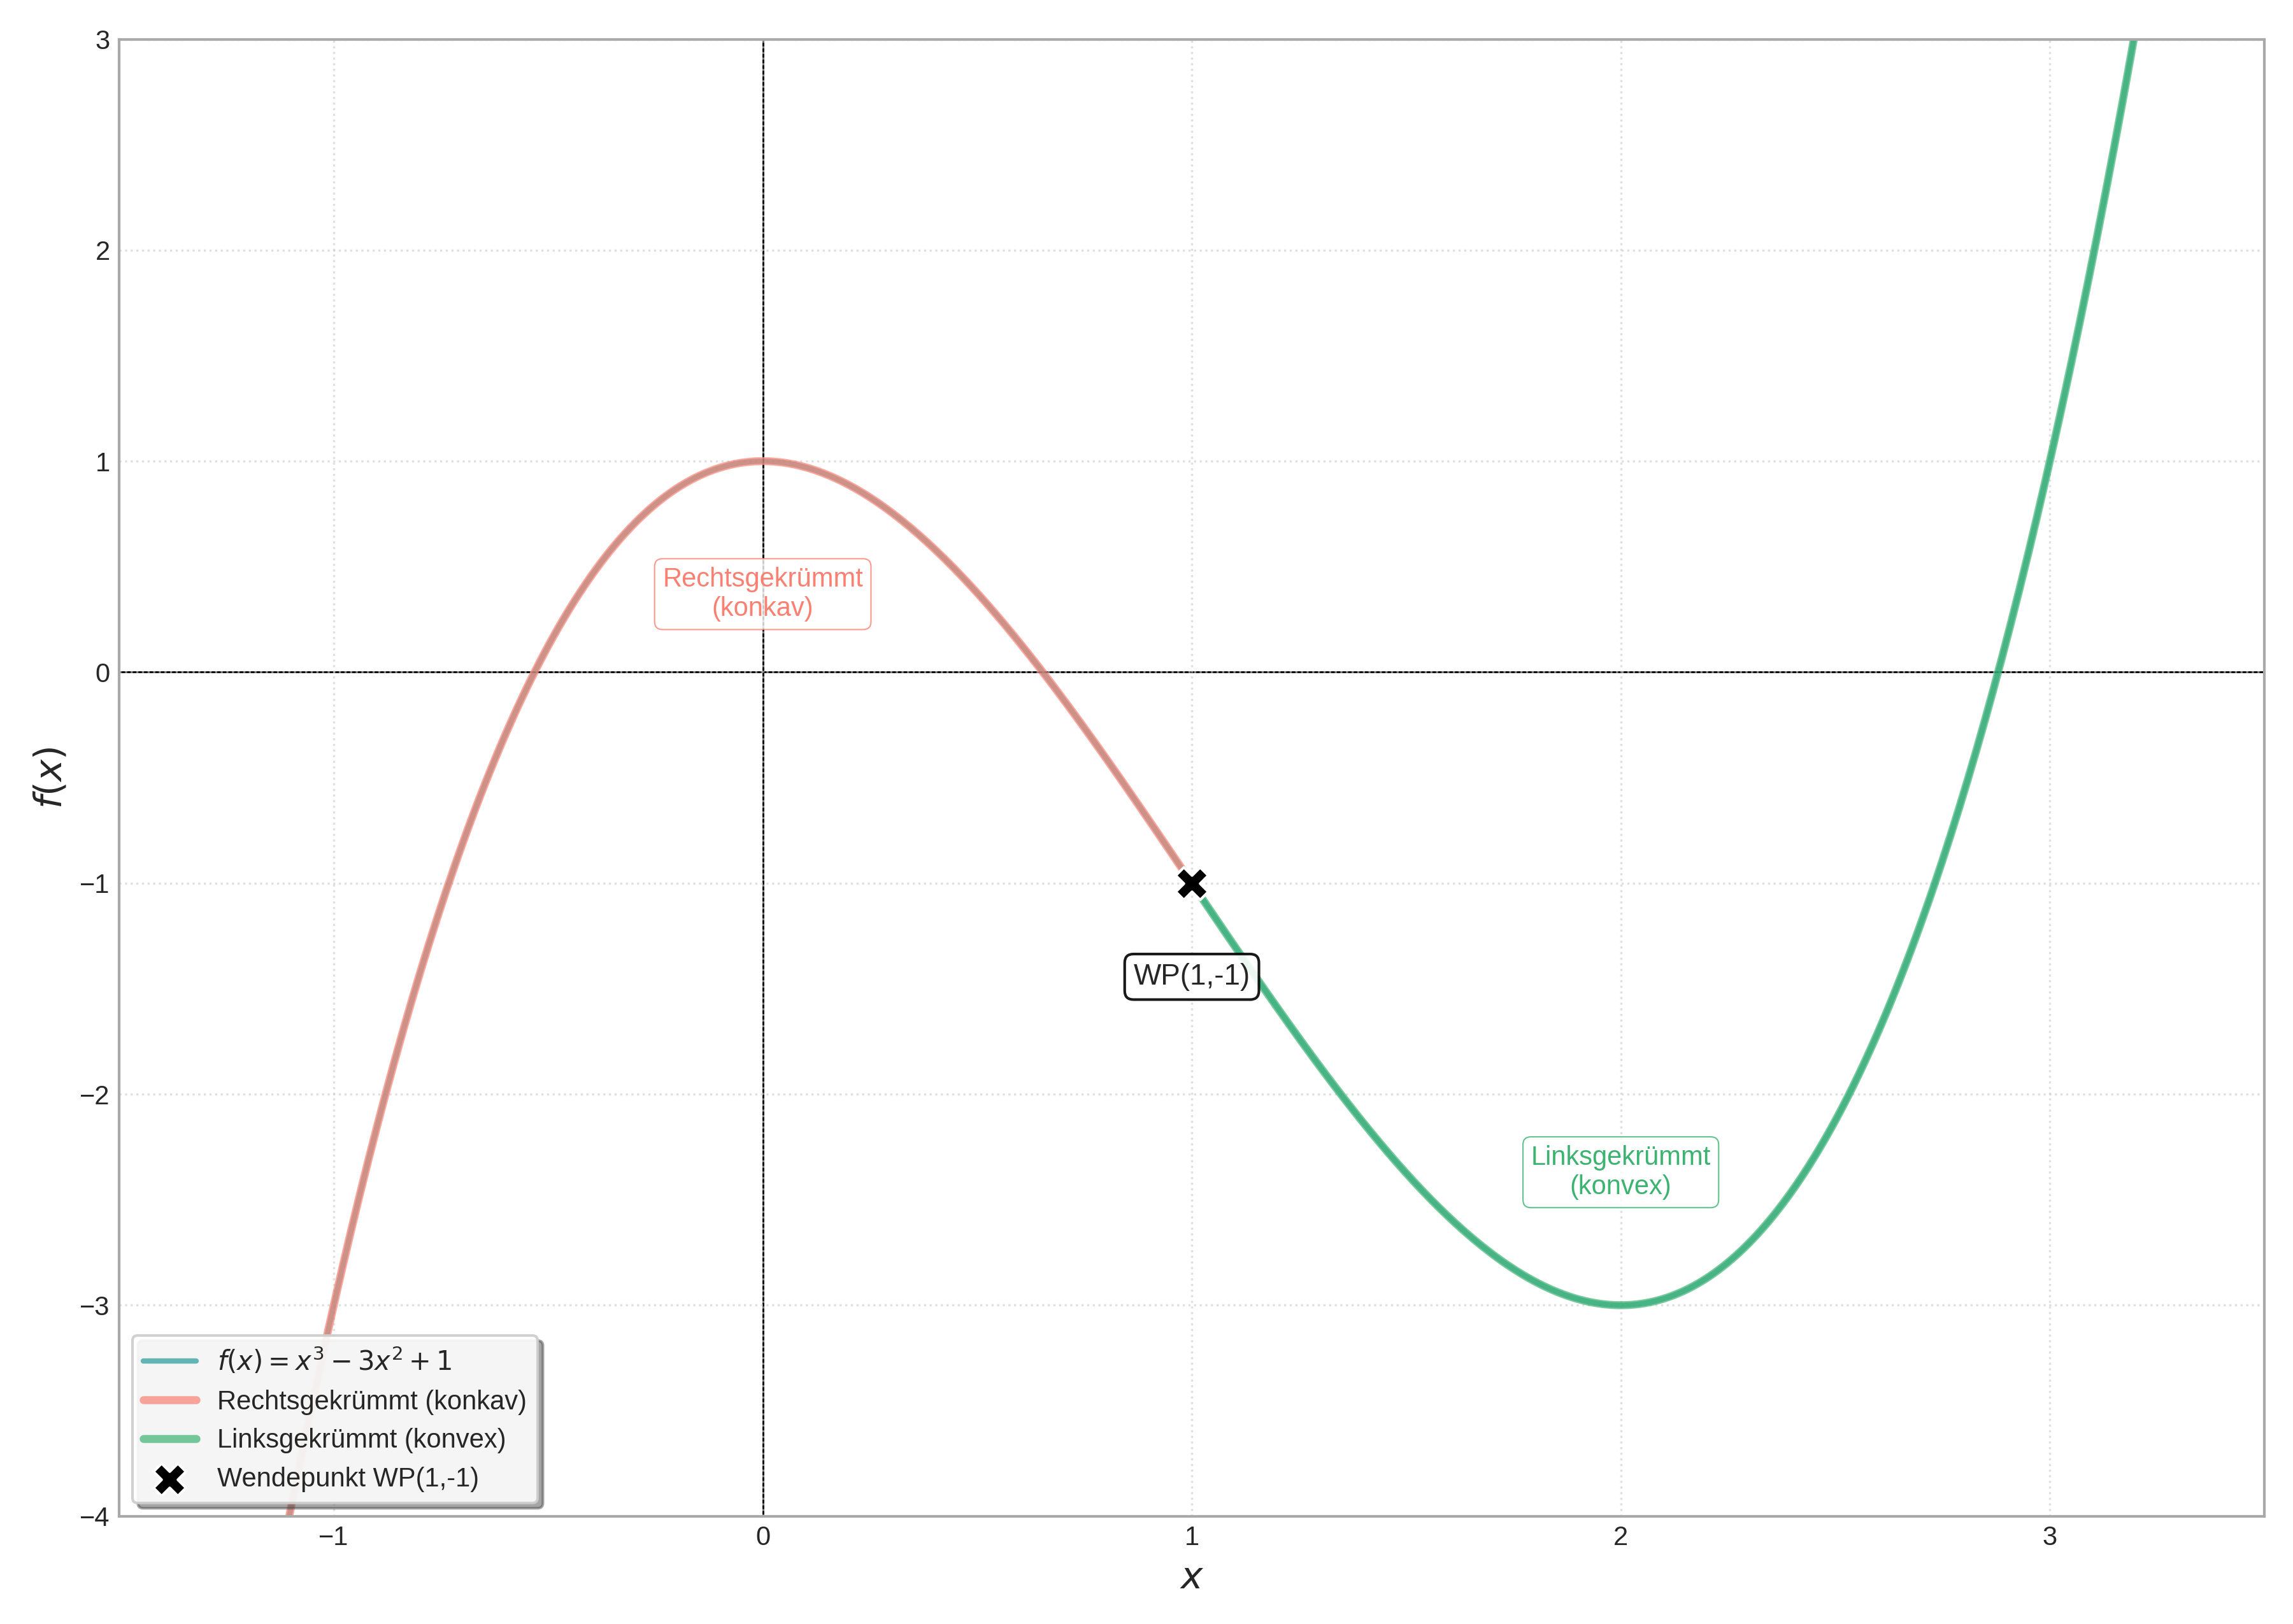
\includegraphics[width=0.8\textwidth]{grafiken/Differentialrechnung_Kruemmung.png}
    \captionof{figure}{Krümmungsverhalten von $f(x)=x^3-3x^2+1$}
    \label{fig:kruemmung_bsp_neu}
\end{center}


\end{beispielumgebung}

\subsubsection{Wendepunkte – Wo die Kurve ihre Richtung ändert}
Ein \textbf{Wendepunkt} ist ein Punkt auf dem Graphen einer Funktion, an dem sich das Krümmungsverhalten ändert. Das bedeutet, der Graph wechselt dort von einer Linkskurve in eine Rechtskurve oder umgekehrt. Die Tangente an diesem Punkt nennt man \textbf{Wendetangente}.

\begin{merksatzumgebung}{Wendepunkte finden}
Um Wendepunkte einer Funktion $f(x)$ zu finden (die mindestens zweimal differenzierbar sein muss):

\textbf{1. Notwendige Bedingung für Wendepunkte:}
Wenn $f(x)$ an der Stelle $x_W$ einen Wendepunkt hat, dann muss gelten:
\[ f''(x_W) = 0 \]
Die Stellen $x_W$, an denen $f''(x_W)=0$ ist, sind \textbf{potentielle Wendestellen}.

\textbf{2. Hinreichende Bedingung für Wendepunkte:}
Es gibt zwei gängige hinreichende Bedingungen, um zu bestätigen, dass an einer potentiellen Wendestelle $x_W$ tatsächlich ein Wendepunkt vorliegt:
\begin{itemize}
    \item \textbf{Vorzeichenwechselkriterium von $f''(x)$:}
    Wenn $f''(x)$ an der Stelle $x_W$ einen Vorzeichenwechsel hat (von $+$ nach $-$ oder von $-$ nach $+$), dann liegt bei $x_W$ ein Wendepunkt vor.
    \item \textbf{Mit der dritten Ableitung $f'''(x)$:}
    Wenn $f''(x_W)=0$ und zusätzlich $f'''(x_W) \neq 0$ ist, dann liegt bei $x_W$ ein Wendepunkt vor. (Diese Bedingung ist oft einfacher zu prüfen, wenn die dritte Ableitung leicht zu bilden ist und nicht Null ist.)
\end{itemize}
Die y-Koordinate des Wendepunktes erhältst du, indem du $x_W$ in die Originalfunktion $f(x)$ einsetzt: $y_W = f(x_W)$. Der Wendepunkt ist dann $W(x_W|y_W)$.
\end{merksatzumgebung}
\begin{infoboxumgebung}{Wendepunkte – Mehr als nur ein Krümmungswechsel}
Wir haben gelernt, dass an einem Wendepunkt $x_W$ die zweite Ableitung $f''(x_W)=0$ ist (und $f'''(x_W) \neq 0$ oder ein Vorzeichenwechsel von $f''$ stattfindet). Das bedeutet, die Krümmung des Graphen wechselt dort ihr Vorzeichen (z.B. von einer Rechts- in eine Linkskurve). Aber was bedeutet das für die Steigung der Funktion, also für $f'(x)$?

\textbf{Der Wendepunkt als Extremum der Steigung:}
Da $f''(x)$ die Ableitung von $f'(x)$ ist, bedeutet $f''(x_W)=0$ und ein Vorzeichenwechsel von $f''(x)$ bei $x_W$ (oder $f'''(x_W) \neq 0$), dass die \textbf{erste Ableitung $f'(x)$ an der Stelle $x_W$ eine Extremstelle} hat!
\begin{itemize}
    \item Wechselt $f''(x)$ von $-$ nach $+$ (also der Graph von $f(x)$ von rechts- zu linkskrümmt), dann hat $f'(x)$ bei $x_W$ ein \textit{Minimum}. Die Steigung von $f(x)$ ist an dieser Stelle am geringsten (d.h. am stärksten negativ oder am wenigsten positiv).
    \item Wechselt $f''(x)$ von $+$ nach $-$ (also der Graph von $f(x)$ von links- zu rechtskrümmt), dann hat $f'(x)$ bei $x_W$ ein \textit{Maximum}. Die Steigung von $f(x)$ ist an dieser Stelle am größten.
\end{itemize}
Ein Wendepunkt ist also eine Stelle, an der die \textbf{Steigung des Graphen von $f(x)$ am extremsten} ist (entweder maximal oder minimal im lokalen Sinne).

\textbf{Intuition – Der Weg zwischen den 'Gipfeln und Tälern':}
Stell dir vor, ein Graph hat einen Hochpunkt (Steigung 0) und danach einen Tiefpunkt (Steigung 0). Dazwischen muss die Steigung von 0 erst negativ geworden sein (bergab) und dann wieder weniger negativ, um beim Tiefpunkt wieder 0 zu werden. Irgendwo auf diesem Weg muss die Steigung ihren negativsten (minimalen) Wert erreicht haben – genau das ist der Wendepunkt! Die Straße macht dort die 'schärfste Kurve' nach unten. Analoges gilt für den Übergang von einem Tief- zu einem Hochpunkt.

\textbf{Sattelpunkte als Spezialfall:}
Wenn an einem Wendepunkt $x_W$ zusätzlich gilt, dass $f'(x_W)=0$ ist (die Tangente also waagerecht ist), dann nennen wir diesen Punkt einen \textbf{Sattelpunkt}. Hier ist die Steigung nicht nur extrem (nämlich 0), sondern es findet auch ein Krümmungswechsel statt, aber kein Monotoniewechsel der Funktion $f(x)$ selbst.

Die Betrachtung des Wendepunkts als Extremum der ersten Ableitung kann helfen, sein Auftreten und seine Bedeutung besser zu verstehen. Es ist ein schönes Beispiel dafür, wie die verschiedenen Ableitungen zusammenwirken, um das Verhalten einer Funktion zu beschreiben.
\end{infoboxumgebung}
\begin{beispielumgebung}{Wendepunkt bestimmen}
Bestimme den Wendepunkt von $f(x) = x^3 - 3x^2 + 1$.
Wir hatten:
$f'(x) = 3x^2 - 6x$
$f''(x) = 6x - 6$

\textbf{Schritt 1: Notwendige Bedingung $f''(x_W)=0$.}
$6x_W - 6 = 0 \implies 6x_W = 6 \implies x_W = 1$.
Die potentielle Wendestelle ist bei $x_W=1$.

\textbf{Schritt 2: Hinreichende Bedingung prüfen.}
\textit{Möglichkeit a) Vorzeichenwechsel von $f''(x)$:}
Wir hatten bereits im vorherigen Beispiel gesehen:
Links von $x=1$ (z.B. $x=0$): $f''(0) = -6 < 0$ (rechtsgekrümmt).
Rechts von $x=1$ (z.B. $x=2$): $f''(2) = 6 > 0$ (linksgekrümmt).
Da ein Vorzeichenwechsel von $f''(x)$ von $-$ nach $+$ an der Stelle $x=1$ stattfindet, liegt dort ein Wendepunkt vor.

\textit{Möglichkeit b) Mit der dritten Ableitung $f'''(x)$:}
$f'''(x) = (f''(x))' = (6x-6)' = 6$.
Nun setzen wir $x_W=1$ in $f'''(x)$ ein:
$f'''(1) = 6$.
Da $f'''(1) = 6 \neq 0$ (und $f''(1)=0$ war), liegt bei $x_W=1$ ein Wendepunkt vor.

\textbf{Schritt 3: y-Koordinate des Wendepunkts berechnen.}
$y_W = f(x_W) = f(1) = (1)^3 - 3(1)^2 + 1 = 1 - 3 + 1 = -1$.
Der Wendepunkt ist $W(1|-1)$.

Am Wendepunkt $W(1|-1)$ wechselt der Graph von $f(x)=x^3-3x^2+1$ von einer Rechtskrümmung in eine Linkskrümmung.
\begin{center}
    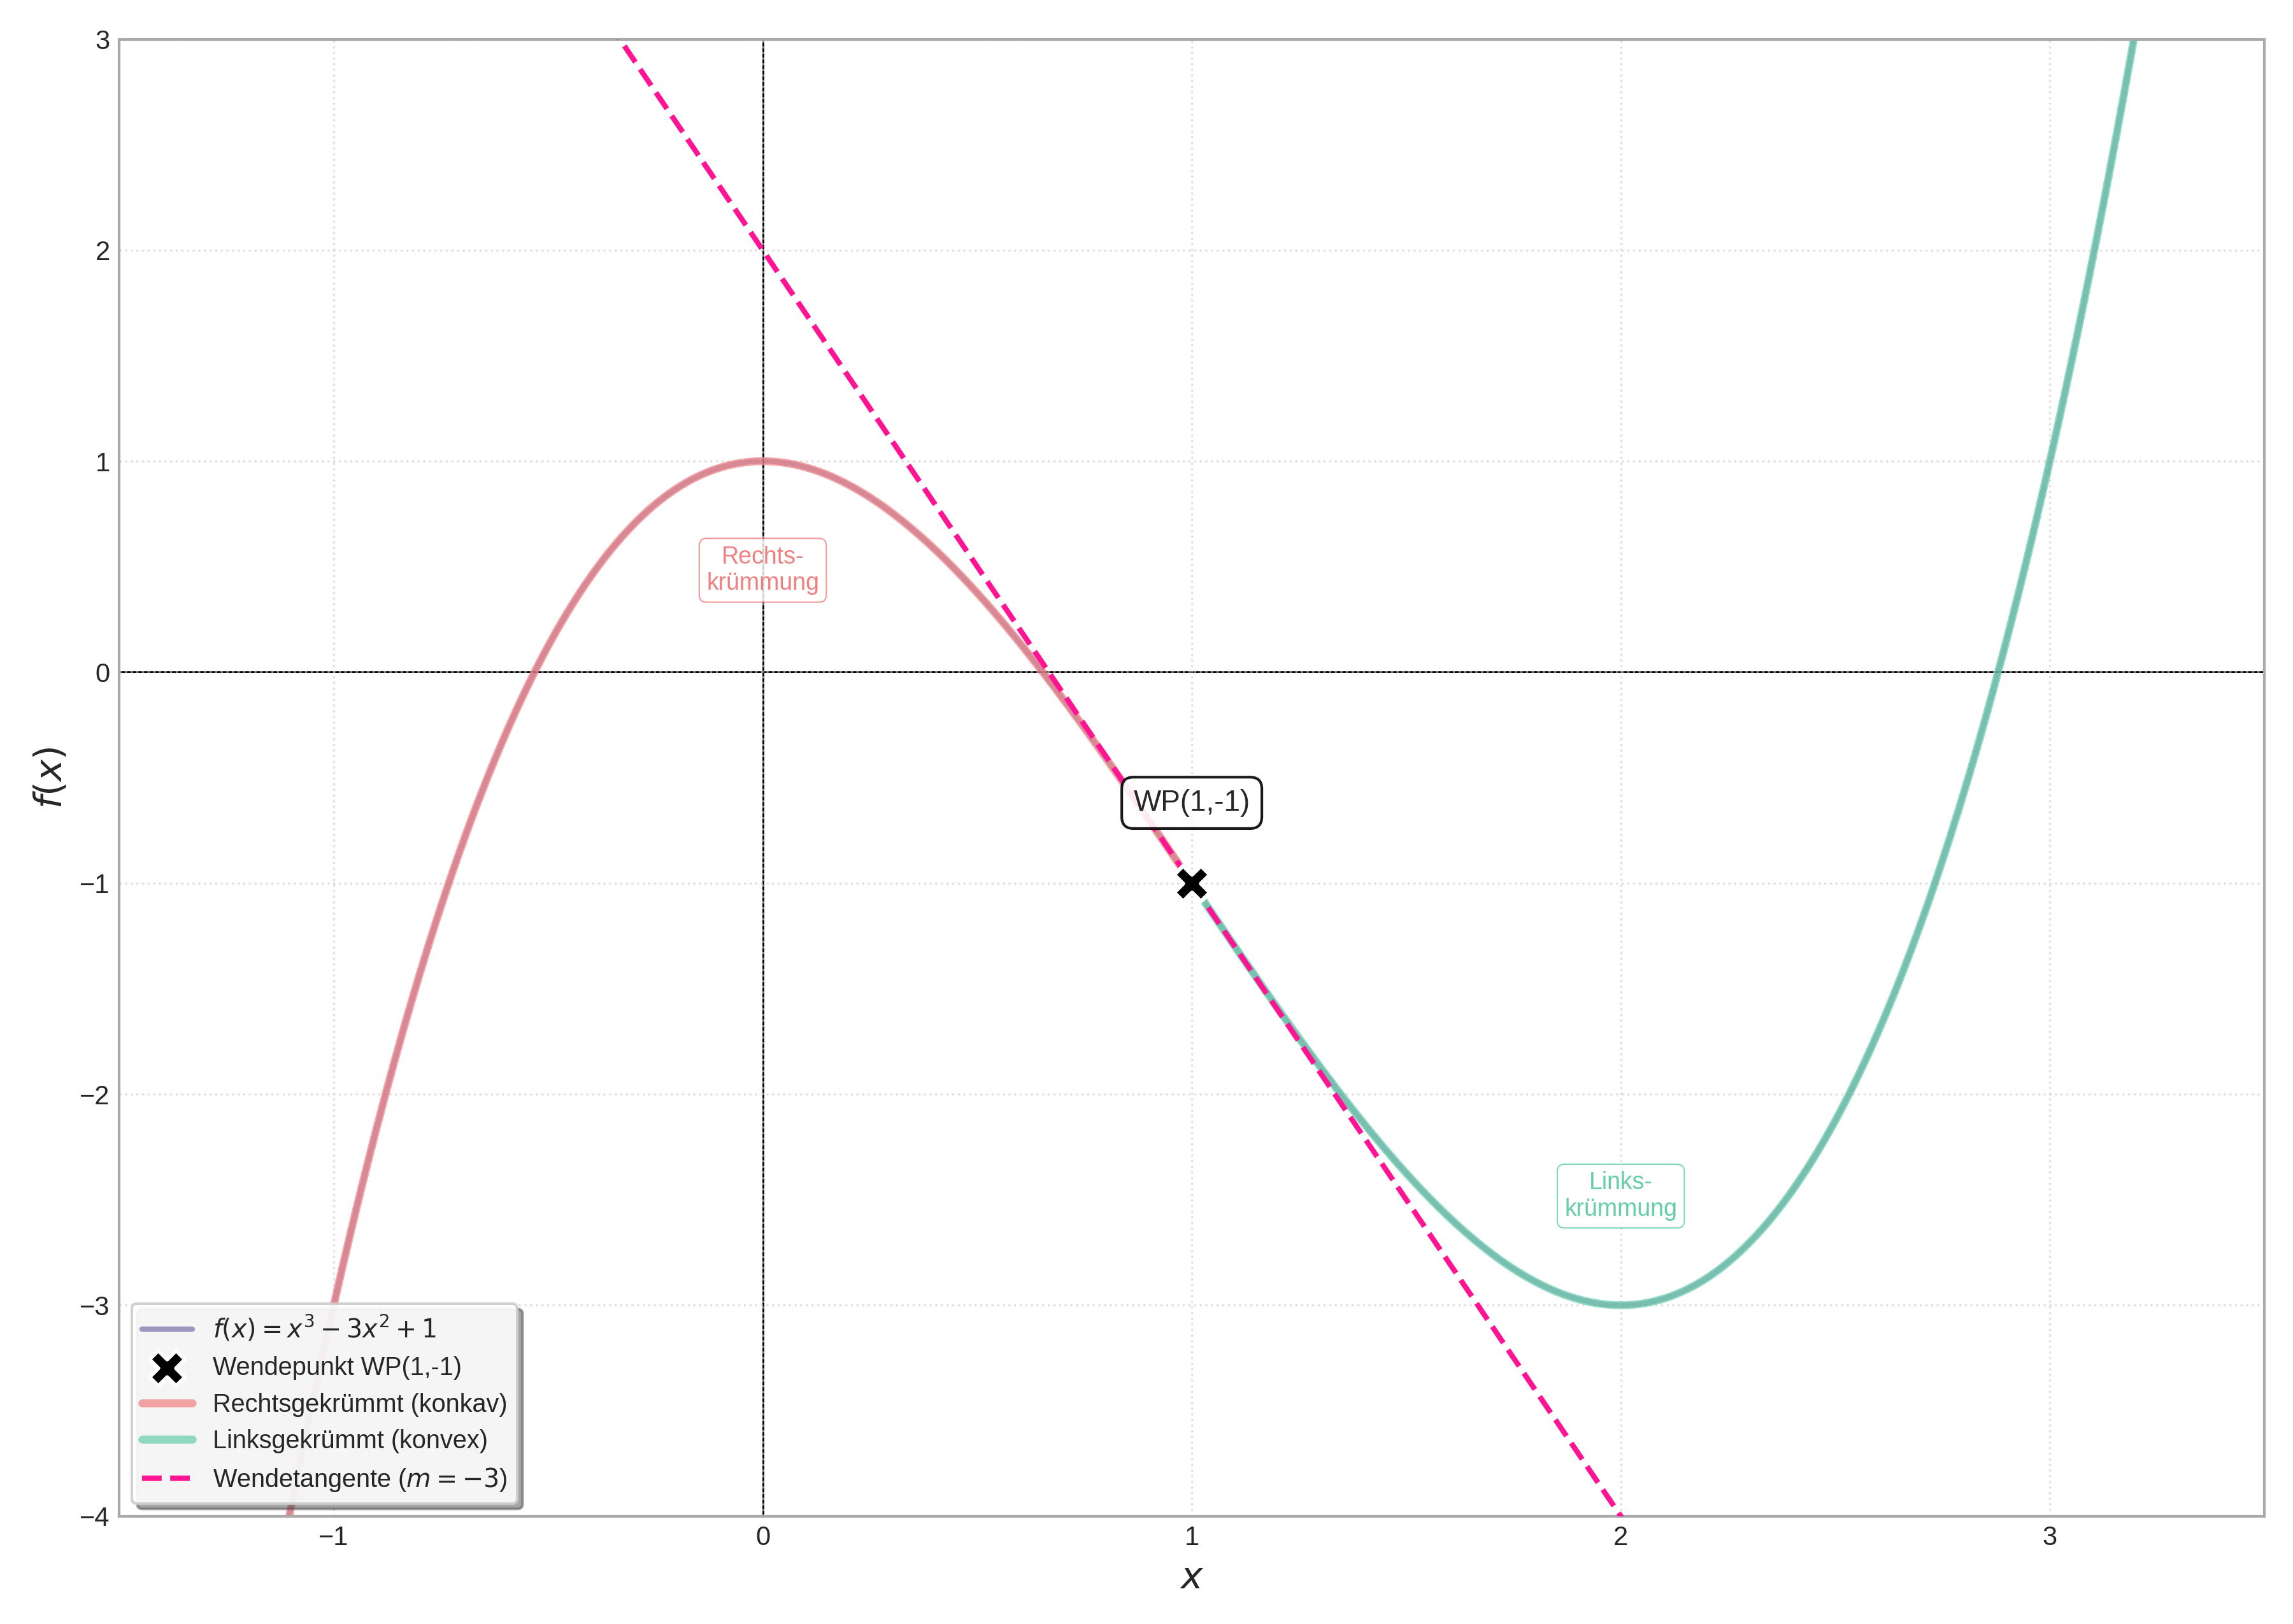
\includegraphics[width=0.8\textwidth]{grafiken/Differentialrechnung_Wendepunkt.png}
    \captionof{figure}{Wendepunkt von $f(x)=x^3-3x^2+1$}
    \label{fig:wendepunkt_bsp}
\end{center}
\end{beispielumgebung}

\begin{tippumgebung}{Zweite Ableitung für Extremstellen}
Die zweite Ableitung kann auch als hinreichende Bedingung für Extremstellen dienen (anstelle des Vorzeichenwechsels von $f'$):
Sei $x_E$ eine Stelle mit $f'(x_E)=0$.
\begin{itemize}
    \item Wenn $f''(x_E) < 0 \implies$ Lokaler Hochpunkt bei $x_E$. (Der Graph ist dort rechtsgekrümmt, wie ein Bergipfel).
    \item Wenn $f''(x_E) > 0 \implies$ Lokaler Tiefpunkt bei $x_E$. (Der Graph ist dort linksgekrümmt, wie ein Talboden).
    \item Wenn $f''(x_E) = 0 \implies$ Keine Aussage möglich mit diesem Kriterium! Dann muss man das Vorzeichenwechselkriterium von $f'$ verwenden. Es könnte ein Sattelpunkt oder doch ein Extremum sein.
\end{itemize}
\end{tippumgebung}

\begin{aufgabenumgebung}{Krümmung und Wendepunkte – Vielfältige Untersuchungen}
Untersuche die folgenden Funktionen auf ihr Krümmungsverhalten (Intervalle für Links- und Rechtskrümmung) und bestimme gegebenenfalls die Koordinaten der Wendepunkte. Nutze dazu die zweite und, falls nötig, die dritte Ableitung.
\begin{enumerate}
    \item $f_1(x) = \frac{1}{12}x^4 - \frac{1}{2}x^3 + x^2 + 1$
        \begin{tippumgebung}{Polynom 4. Grades}
        Die zweite Ableitung $f_1''(x)$ wird eine quadratische Funktion sein. Deren Nullstellen (potentielle Wendestellen) findest du mit den bekannten Lösungsformeln. Überprüfe die hinreichende Bedingung für Wendepunkte.
        \end{tippumgebung}

    \item $f_2(x) = x^5 - 5x^4 + 3x - 2$
        \begin{tippumgebung}{Polynom 5. Grades}
        Die zweite Ableitung $f_2''(x)$ wird ein Polynom 3. Grades sein. Versuche, $x$ (oder eine höhere Potenz von $x$) auszuklammern, um die Nullstellen von $f_2''(x)$ zu finden.
        \end{tippumgebung}

    \item \textbf{Anwendung: Infektionsgeschehen} \\
        Die Funktion $N(t) = -t^3 + 12t^2 + 20t$ beschreibt die Anzahl der neu infizierten Personen pro Tag während einer Grippewelle ($t$ in Tagen, $t \ge 0$).
        \begin{itemize}
            \item Bestimme die Funktion $N'(t)$, welche die Änderungsrate der Neuinfektionen (also die 'Geschwindigkeit' der Ausbreitung) beschreibt.
            \item Bestimme die Funktion $N''(t)$, welche die Änderungsrate der Wachstumsrate der Neuinfektionen beschreibt.
            \item Zu welchem Zeitpunkt $t_W$ ist die Zunahme der täglichen Neuinfektionen am größten? (Das bedeutet, $N'(t)$ hat ein Maximum, also suche einen Wendepunkt von $N(t)$, an dem die Krümmung von links nach rechts wechselt, d.h. $N''(t_W)=0$ und $N'''(t_W)<0$).
            \item Interpretiere die Bedeutung dieses Zeitpunktes $t_W$ für den Verlauf der Grippewelle. Was passiert mit der Zunahme der Neuinfektionen nach diesem Zeitpunkt?
        \end{itemize}

    \item \textbf{Schwer: Funktion mit Parameter $a$} \\
        Gegeben ist die Funktionenschar $f_a(x) = x^4 + ax^3$ mit $a \in \mathbb{R}, a \neq 0$.
        \begin{itemize}
            \item Bestimme die zweite Ableitung $f_a''(x)$.
            \item Zeige, dass $x_1=0$ eine potentielle Wendestelle ist. Untersuche mit der dritten Ableitung $f_a'''(x)$, ob für $x_1=0$ tatsächlich ein Wendepunkt vorliegt.
            \item Bestimme die andere potentielle Wendestelle $x_2$ in Abhängigkeit von $a$.
            \item Für welche Werte von $a$ existiert dieser zweite Wendepunkt $x_2$? (Beachte, dass $x_2 \neq x_1$ sein sollte für einen \textit{anderen} Wendepunkt).
            \item Untersuche das Krümmungsverhalten für $a=2$ und $a=-2$ und skizziere grob die Verläufe (ohne vollständige Kurvendiskussion, Fokus auf Krümmung und Wendepunkte).
        \end{itemize}
        \begin{tippumgebung}{Parameter $a$}
        Behandle $a$ wie eine Konstante beim Ableiten. Die Ergebnisse für Wendestellen und Krümmungsintervalle werden dann von $a$ abhängen.
        \end{tippumgebung}
\end{enumerate}
\end{aufgabenumgebung}

% Dieser Block sollte im Kapitel 'Einführung in die Differentialrechnung',
% nach der aufgabenumgebung 'Krümmung und Wendepunkte – Vielfältige Untersuchungen'
% und vor dem \subsection 'Grenzwerte (Limes)...' eingefügt werden.

\subsubsection{Tangenten und Normalen – Geraden am Graphen}
\label{subsubsec:tangenten_normalen}

Wir wissen bereits, dass die erste Ableitung $f'(x_0)$ die Steigung der Tangente an den Graphen der Funktion $f(x)$ im Punkt $P(x_0|f(x_0))$ angibt. Mit diesem Wissen können wir die Gleichung dieser Tangente und auch die Gleichung der Normalen (die Senkrechte zur Tangente im selben Punkt) bestimmen.

\begin{merksatzumgebung}{Gleichung der Tangente}
Die Gleichung der Tangente $t(x)$ an den Graphen einer Funktion $f(x)$ im Punkt $P(x_0|y_0)$ mit $y_0=f(x_0)$ lautet:
\[ t(x) = f'(x_0) \cdot (x - x_0) + y_0 \]
oder
\[ t(x) = f'(x_0) \cdot (x - x_0) + f(x_0) \]
Dabei ist $m_T = f'(x_0)$ die Steigung der Tangente. Diese Formel ist die Punkt-Steigungs-Form einer Geraden.
\end{merksatzumgebung}

\begin{merksatzumgebung}{Gleichung der Normale}
Die Normale $n(x)$ ist die Gerade, die senkrecht zur Tangente $t(x)$ im Punkt $P(x_0|y_0)$ steht.
Für die Steigungen $m_T$ der Tangente und $m_N$ der Normalen gilt (wenn $m_T \neq 0$): $m_N = -\frac{1}{m_T}$.
Die Gleichung der Normalen $n(x)$ im Punkt $P(x_0|y_0)$ mit $y_0=f(x_0)$ lautet also, falls $f'(x_0) \neq 0$:
\[ n(x) = -\frac{1}{f'(x_0)} \cdot (x - x_0) + y_0 \]
Falls $f'(x_0) = 0$ (horizontale Tangente, z.B. an Extrempunkten), ist die Tangente $y=y_0$ und die Normale eine senkrechte Gerade $x=x_0$.
\end{merksatzumgebung}

\begin{tippumgebung}{Tangenten und Normalen an besonderen Punkten}
\begin{itemize}
    \item \textbf{An Extrempunkten ($f'(x_E)=0$):}
        Die Tangente ist waagerecht: $t(x) = f(x_E)$.
        Die Normale ist senkrecht: $x = x_E$ (keine Funktion der Form $y=mx+b$).
        Die Berechnung einer Normalen\textit{gleichung} in der Form $y=mx+b$ ist hier also nicht sinnvoll, aber die Normale existiert als senkrechte Linie.
    \item \textbf{An Wendepunkten ($W(x_W|f(x_W))$):}
        Die Tangente im Wendepunkt wird \textbf{Wendetangente} genannt. Ihre Steigung $f'(x_W)$ ist oft die größte oder kleinste Steigung in der Umgebung des Wendepunkts.
        Die Normale im Wendepunkt wird \textbf{Wendenormale} genannt.
    \item \textbf{An beliebigen Punkten:} Man kann die Tangente und Normale an \textit{jedem} Punkt des Graphen berechnen, an dem die Funktion differenzierbar ist, nicht nur an ausgezeichneten Punkten wie Extrema oder Wendepunkten.
\end{itemize}
\end{tippumgebung}

\begin{beispielumgebung}{Wendetangente und Wendenormale berechnen}
Wir betrachten wieder die Funktion $f(x) = x^3 - 3x^2 + 1$.
Aus einem früheren Beispiel wissen wir:
$f'(x) = 3x^2 - 6x$
$f''(x) = 6x - 6$
$f'''(x) = 6$
Der Wendepunkt liegt bei $x_W=1$, mit $f(1) = 1-3+1 = -1$. Also $W(1|-1)$.

\textbf{1. Wendetangente $t_W(x)$ im Punkt $W(1|-1)$:}
Steigung im Wendepunkt: $m_T = f'(1) = 3(1)^2 - 6(1) = 3 - 6 = -3$.
Punkt-Steigungs-Form: $t_W(x) = m_T (x - x_W) + f(x_W)$
$t_W(x) = -3 (x - 1) + (-1)$
$t_W(x) = -3x + 3 - 1$
\[ t_W(x) = -3x + 2 \]

\textbf{2. Wendenormale $n_W(x)$ im Punkt $W(1|-1)$:}
Steigung der Tangente war $m_T = -3$.
Steigung der Normalen: $m_N = -\frac{1}{m_T} = -\frac{1}{-3} = \frac{1}{3}$.
Punkt-Steigungs-Form: $n_W(x) = m_N (x - x_W) + f(x_W)$
$n_W(x) = \frac{1}{3} (x - 1) + (-1)$
$n_W(x) = \frac{1}{3}x - \frac{1}{3} - 1$
$n_W(x) = \frac{1}{3}x - \frac{1}{3} - \frac{3}{3}$
\[ n_W(x) = \frac{1}{3}x - \frac{4}{3} \]
\begin{center}
    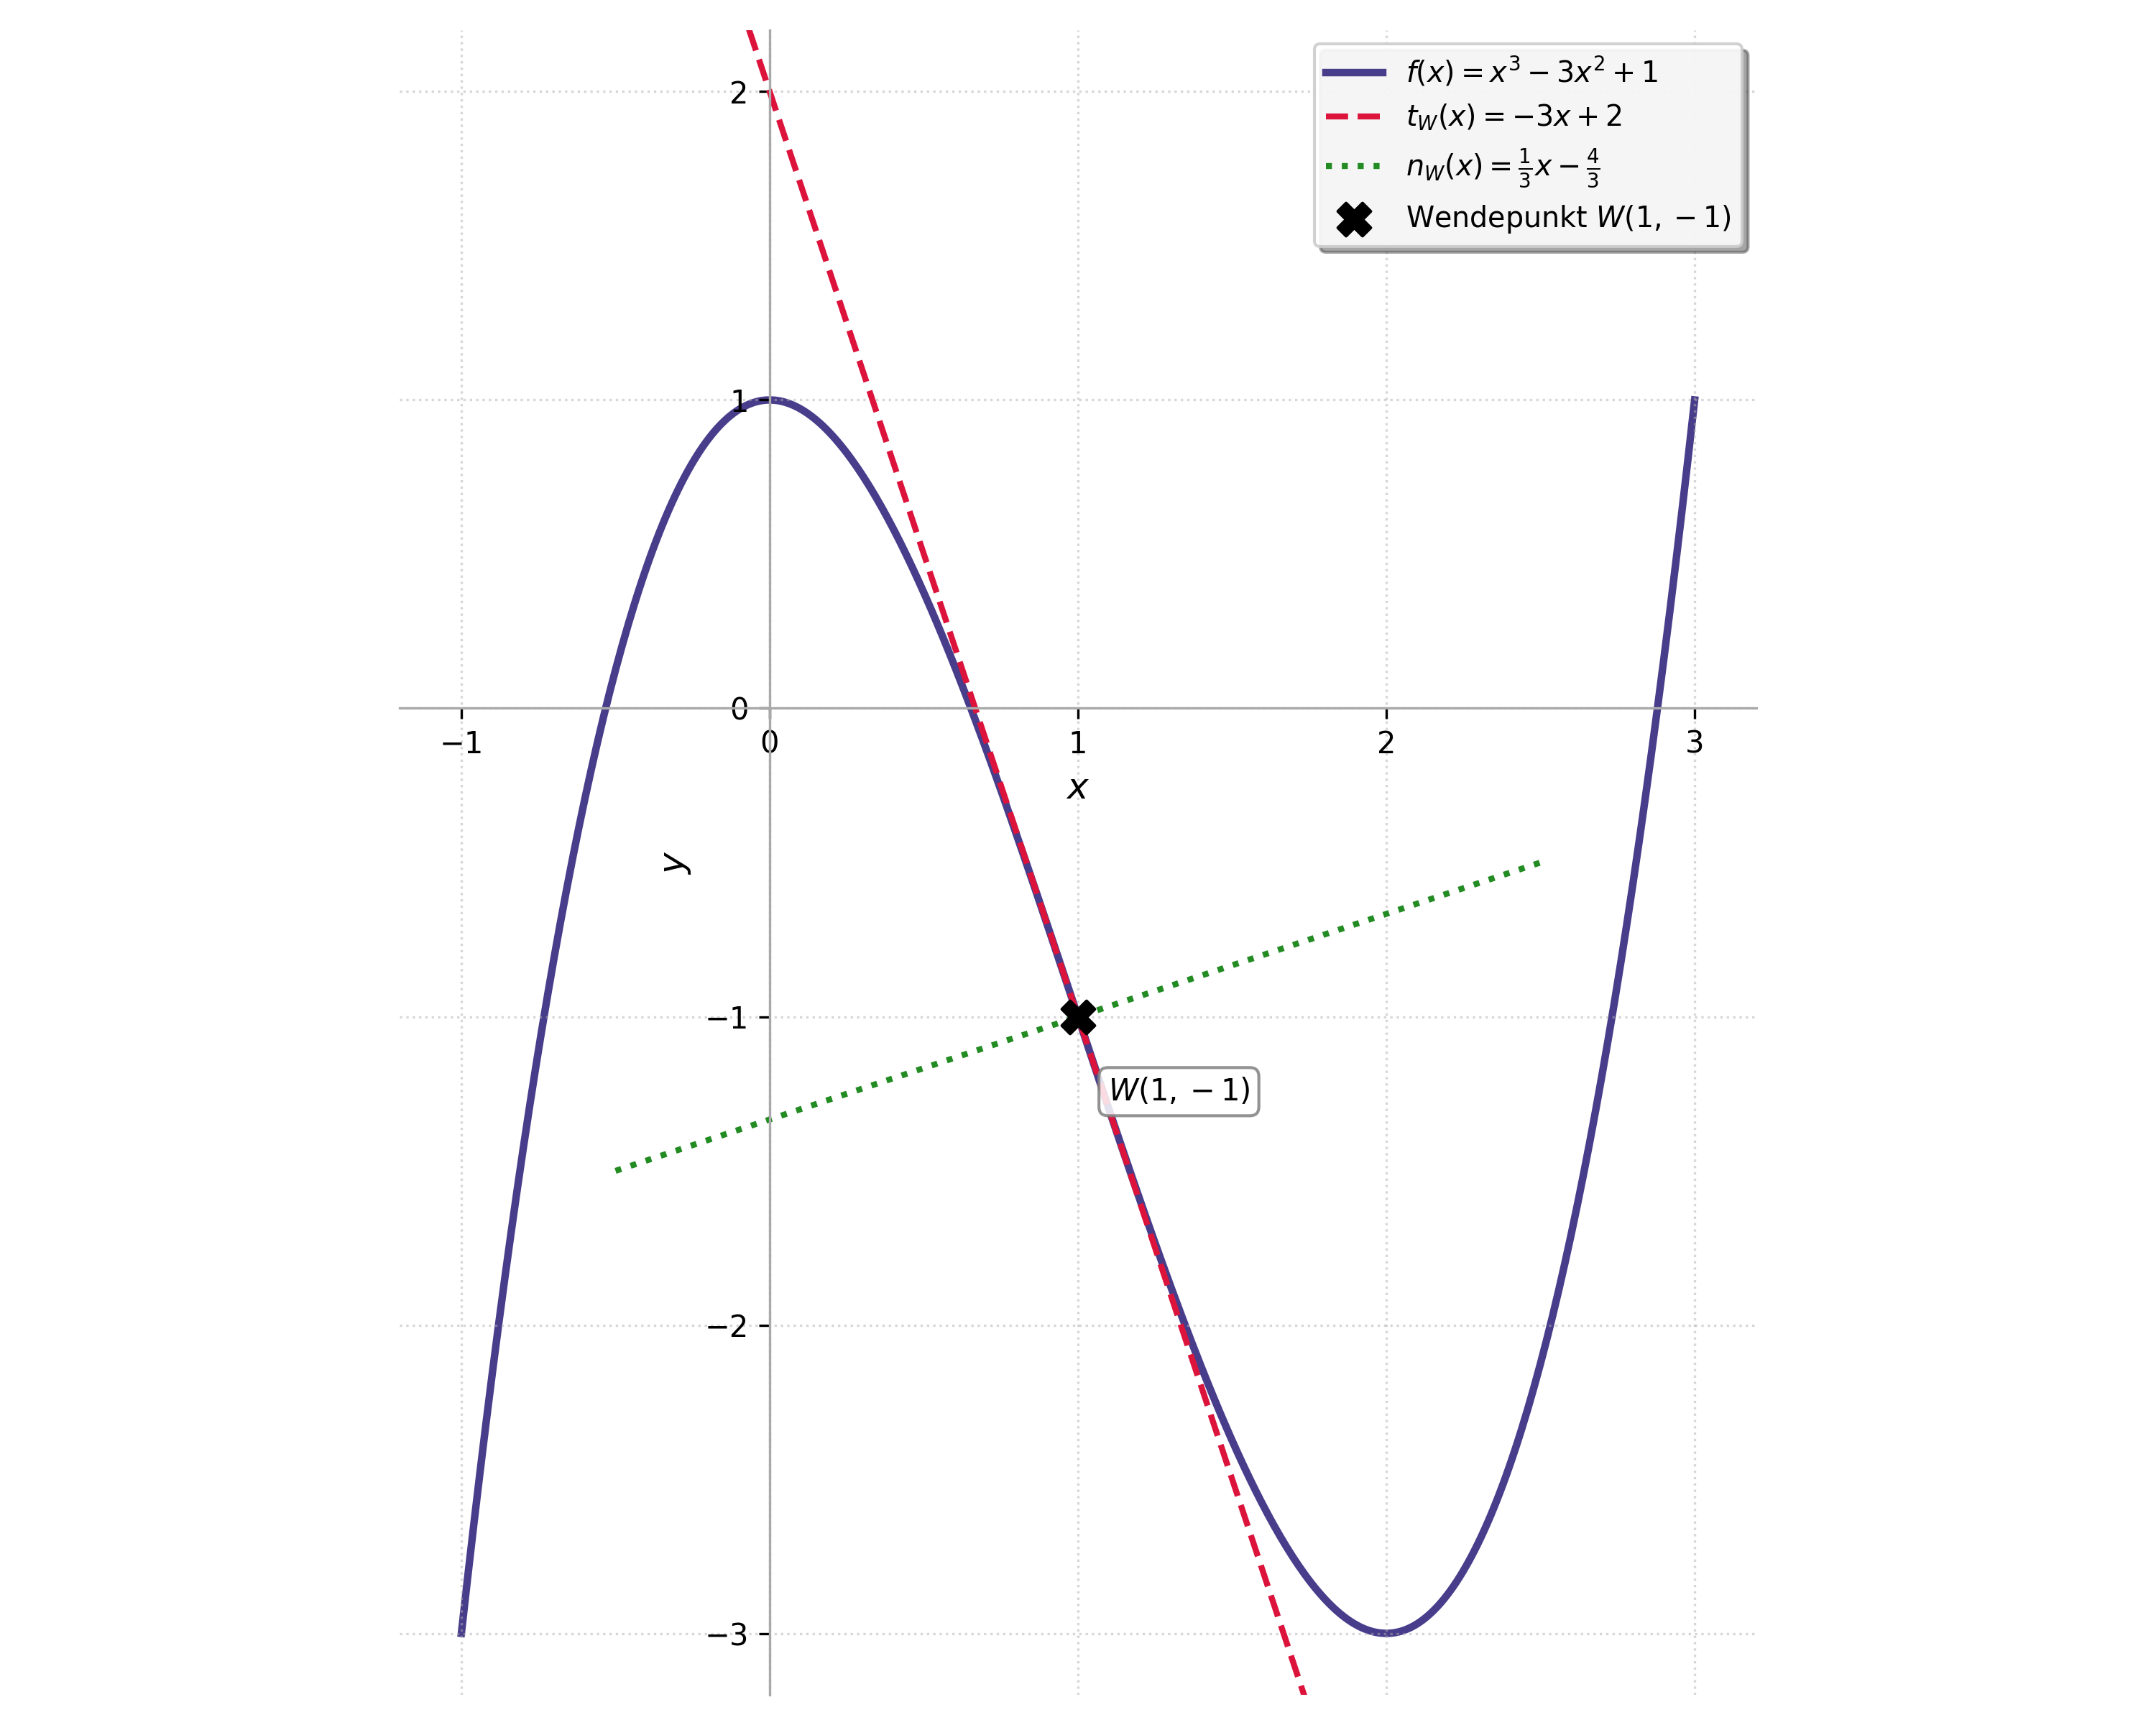
\includegraphics[width=0.8\textwidth]{grafiken/Wendetangente_Normale.png}
    \captionof{figure}{Wendetangente und Wendenormale für $f(x)=x^3-3x^2+1$ im Punkt $W(1|-1)$}
    \label{fig:wendetangente_normale}
\end{center}
\end{beispielumgebung}

\begin{aufgabenumgebung}{Tangenten und Normalen bestimmen – Vielfältige Aufgaben}
\begin{enumerate}
    \item Gegeben ist die Funktion $f(x) = \frac{1}{4}x^4 - x^2 + 1$.
        \begin{itemize}
            \item Bestimme die Gleichung der Tangente und der Normalen an den Graphen von $f$ an der Stelle $x_0 = 2$.
            \item An welchen Stellen $x$ hat der Graph von $f$ eine Tangente mit der Steigung $m=0$? Was für Punkte sind das?
            \item (Schwer): Gibt es eine Tangente an den Graphen von $f$, die parallel zur Geraden $y = -2x+5$ ist? Wenn ja, bestimme die Berührpunkte und die Gleichungen dieser Tangenten.
        \end{itemize}
    \item Gegeben ist die Funktion $g(x) = x^3 - 3x$.
        \begin{itemize}
            \item Bestimme die Wendepunkt(e) von $g(x)$.
            \item Bestimme die Gleichung der Wendetangente(n).
            \item Zeige, dass die Wendetangente im Ursprung (falls vorhanden) die x-Achse nur im Ursprung schneidet.
        \end{itemize}
    \item \textbf{Orthogonale Tangenten (Für Experten):}
        Gegeben ist die Parabel $f(x) = x^2$. Gibt es zwei Punkte $P_1(x_1|f(x_1))$ und $P_2(x_2|f(x_2))$ auf der Parabel, deren Tangenten sich senkrecht schneiden und deren x-Koordinaten die Bedingung $x_1 \cdot x_2 = -1/4$ erfüllen?
        \begin{tippumgebung}{Orthogonalität}
        Zwei Geraden mit Steigungen $m_1$ und $m_2$ sind orthogonal (senkrecht), wenn $m_1 \cdot m_2 = -1$ (vorausgesetzt $m_1, m_2 \neq 0$).
        \end{tippumgebung}
    \item \textbf{Normale durch den Ursprung:}
        Für die Funktion $f(x) = \frac{1}{2}x^2 - 2x + 3$, bestimme den Punkt $P(x_0|f(x_0))$ auf dem Graphen, dessen Normale durch den Ursprung $(0|0)$ verläuft.

    \item \textbf{Wendetangente mit speziellen Eigenschaften (Schwer):}
        Gegeben ist die Funktion $f(x) = \frac{1}{6}x^3 - x^2 + 2x + 1$.
        \begin{itemize}
            \item Bestimme die Koordinaten des Wendepunktes $W$.
            \item Bestimme die Gleichung der Wendetangente $t_W(x)$ und der Wendenormalen $n_W(x)$.
            \item Die Wendetangente, die Wendenormale und die y-Achse bilden ein Dreieck. Berechne den Flächeninhalt dieses Dreiecks.
            \item Unter welchem Winkel schneidet die Wendetangente die x-Achse? (Tipp: Der Tangens des Steigungswinkels $\alpha$ einer Geraden ist gleich ihrer Steigung $m$, also $\tan(\alpha) = m$. Du suchst $\alpha = \arctan(m)$.)
        \end{itemize}

    \item \textbf{Berührbedingung und Parameter (Schwer):}
        Gegeben sind die Funktionen $f(x) = x^2 + 2x + 2$ und die Geradenschar $g_k(x) = kx - 2$ (wobei $k \in \mathbb{R}$ ein Parameter ist).
        \begin{itemize}
            \item Für welchen Wert von $k$ berührt die Gerade $g_k(x)$ die Parabel $f(x)$?
            \begin{tippumgebung}{Berührbedingung}
            Zwei Funktionen $f(x)$ und $g(x)$ berühren sich an einer Stelle $x_B$, wenn gilt:
            \begin{enumerate}
                \item $f(x_B) = g(x_B)$ (gleicher Funktionswert am Berührpunkt)
                \item $f'(x_B) = g'(x_B)$ (gleiche Steigung am Berührpunkt)
            \end{enumerate}
            Du erhältst ein Gleichungssystem für $x_B$ und $k$.
            \end{tippumgebung}
            \item Bestimme den Berührpunkt und die Gleichung der gemeinsamen Tangente für diesen Wert von $k$.
            \item (Für Experten): Gibt es einen Wert für $k$, sodass die Gerade $g_k(x)$ eine Normale zur Parabel $f(x)$ an einem Punkt $P(x_0|f(x_0))$ ist? Wenn ja, bestimme $k$ und den Punkt $P$.
        \end{itemize}
\end{enumerate}
\end{aufgabenumgebung}

% Hier geht es dann weiter mit dem nächsten großen Abschnitt, z.B. Grenzwerten oder weiteren Ableitungsregeln.



\subsubsection{Sattelpunkte – Besondere Wendepunkte mit horizontaler Tangente}
\label{subsubsec:sattelpunkte}

In der Kurvendiskussion haben wir bereits Extrempunkte (Hoch- und Tiefpunkte) und Wendepunkte kennengelernt. Sattelpunkte, auch Terrassenpunkte genannt, sind eine spezielle Art von Wendepunkten, die eine interessante Eigenschaft mit Extrempunkten teilen: Die Tangente an den Graphen ist an einem Sattelpunkt \textbf{waagerecht}, genau wie bei einem Hoch- oder Tiefpunkt. Der Unterschied ist jedoch, dass die Funktion an einem Sattelpunkt ihr Monotonieverhalten \textit{nicht} ändert.

Stell dir vor, du fährst auf einer kurvigen Bergstraße. Ein Hochpunkt ist ein Gipfel, ein Tiefpunkt ein Tal. Ein Wendepunkt ist eine Stelle, an der eine Rechtskurve in eine Linkskurve übergeht (oder umgekehrt). Ein Sattelpunkt ist nun ein Wendepunkt, an dem die Straße für einen kurzen Moment exakt horizontal verläuft, bevor sie ihre Krümmung ändert und in derselben Richtung (steigend oder fallend) weiterführt.

\begin{merksatzumgebung}[def_sattelpunkt]{Definition und Bedingungen für einen Sattelpunkt}
Ein Punkt $S(x_S|f(x_S))$ auf dem Graphen einer Funktion $f(x)$ ist ein \textbf{Sattelpunkt} (oder Terrassenpunkt), wenn folgende Bedingungen erfüllt sind:
\begin{enumerate}
    \item \textbf{Horizontale Tangente:} Die erste Ableitung ist an der Stelle $x_S$ Null.
    \[ f'(x_S) = 0 \]
    (Dies ist die notwendige Bedingung auch für Extremstellen.)
    \item \textbf{Kein Vorzeichenwechsel der ersten Ableitung:} Die erste Ableitung $f'(x)$ wechselt an der Stelle $x_S$ \textbf{nicht} das Vorzeichen. Das bedeutet, die Funktion ist links und rechts von $x_S$ entweder beidesmal steigend oder beidesmal fallend.
    \textit{Alternativ (und oft einfacher zu prüfen mit höheren Ableitungen):}
    \item \textbf{Zweite Ableitung ist Null:} Die zweite Ableitung ist an der Stelle $x_S$ Null.
    \[ f''(x_S) = 0 \]
    (Dies ist die notwendige Bedingung für einen Wendepunkt.)
    \item \textbf{Dritte Ableitung ist ungleich Null:} Die dritte Ableitung an der Stelle $x_S$ ist nicht Null.
    \[ f'''(x_S) \neq 0 \]
    (Dies ist eine hinreichende Bedingung dafür, dass bei $f''(x_S)=0$ tatsächlich ein Wendepunkt vorliegt und kein Extremum höherer Ordnung, bei dem $f''$ zufällig Null ist.)
\end{enumerate}
Zusammenfassend: Ein Sattelpunkt ist ein Wendepunkt mit einer horizontalen Tangente.
\end{merksatzumgebung}

\begin{warumwichtigumgebung}{Sattelpunkte erkennen}
Sattelpunkte sind wichtig, weil sie Stellen markieren, an denen die Steigung kurzzeitig Null wird, ohne dass ein lokales Maximum oder Minimum vorliegt. In Optimierungsprozessen könnten solche Punkte 'falsche Freunde' sein – man denkt, man hat ein Optimum erreicht, aber tatsächlich geht es danach in gleicher Richtung weiter. In der Physik können sie Übergangszustände oder instabile Gleichgewichtslagen repräsentieren.
\end{warumwichtigumgebung}

\begin{beispielumgebung}{Untersuchung auf Sattelpunkte bei \texorpdfstring{$f(x) = x^3$}{f(x) = x hoch 3}}
Die einfachste Funktion mit einem Sattelpunkt im Ursprung ist $f(x) = x^3$.
\begin{enumerate}
    \item \textbf{Ableitungen bilden:}
        $f(x) = x^3$
        $f'(x) = 3x^2$
        $f''(x) = 6x$
        $f'''(x) = 6$

    \item \textbf{Potentielle Stellen für horizontale Tangenten (kritische Stellen):}
        $f'(x) = 0 \implies 3x^2 = 0 \implies x = 0$.
        Einzige kritische Stelle ist $x_S = 0$.

    \item \textbf{Überprüfung mit Vorzeichenwechsel von $f'(x)$:}
        \begin{itemize}
            \item Links von $x=0$ (z.B. $x=-1$): $f'(-1) = 3(-1)^2 = 3 > 0$ (steigend).
            \item Rechts von $x=0$ (z.B. $x=1$): $f'(1) = 3(1)^2 = 3 > 0$ (steigend).
        \end{itemize}
        Da $f'(x)$ bei $x=0$ keinen Vorzeichenwechsel hat (von $+$ nach $+$), liegt hier kein Extrempunkt vor.

    \item \textbf{Überprüfung der Wendepunktbedingungen:}
        $f''(x_S) = f''(0) = 6 \cdot 0 = 0$. (Notwendige Bedingung für Wendepunkt erfüllt).
        $f'''(x_S) = f'''(0) = 6 \neq 0$. (Hinreichende Bedingung für Wendepunkt erfüllt).
        Da $f'(0)=0$ und bei $x=0$ ein Wendepunkt vorliegt, ist $P(0|f(0))$ ein Sattelpunkt.

    \item \textbf{Koordinaten des Sattelpunkts:}
        $f(0) = 0^3 = 0$.
        Der Sattelpunkt ist $S(0|0)$.
\end{enumerate}
\begin{center}
    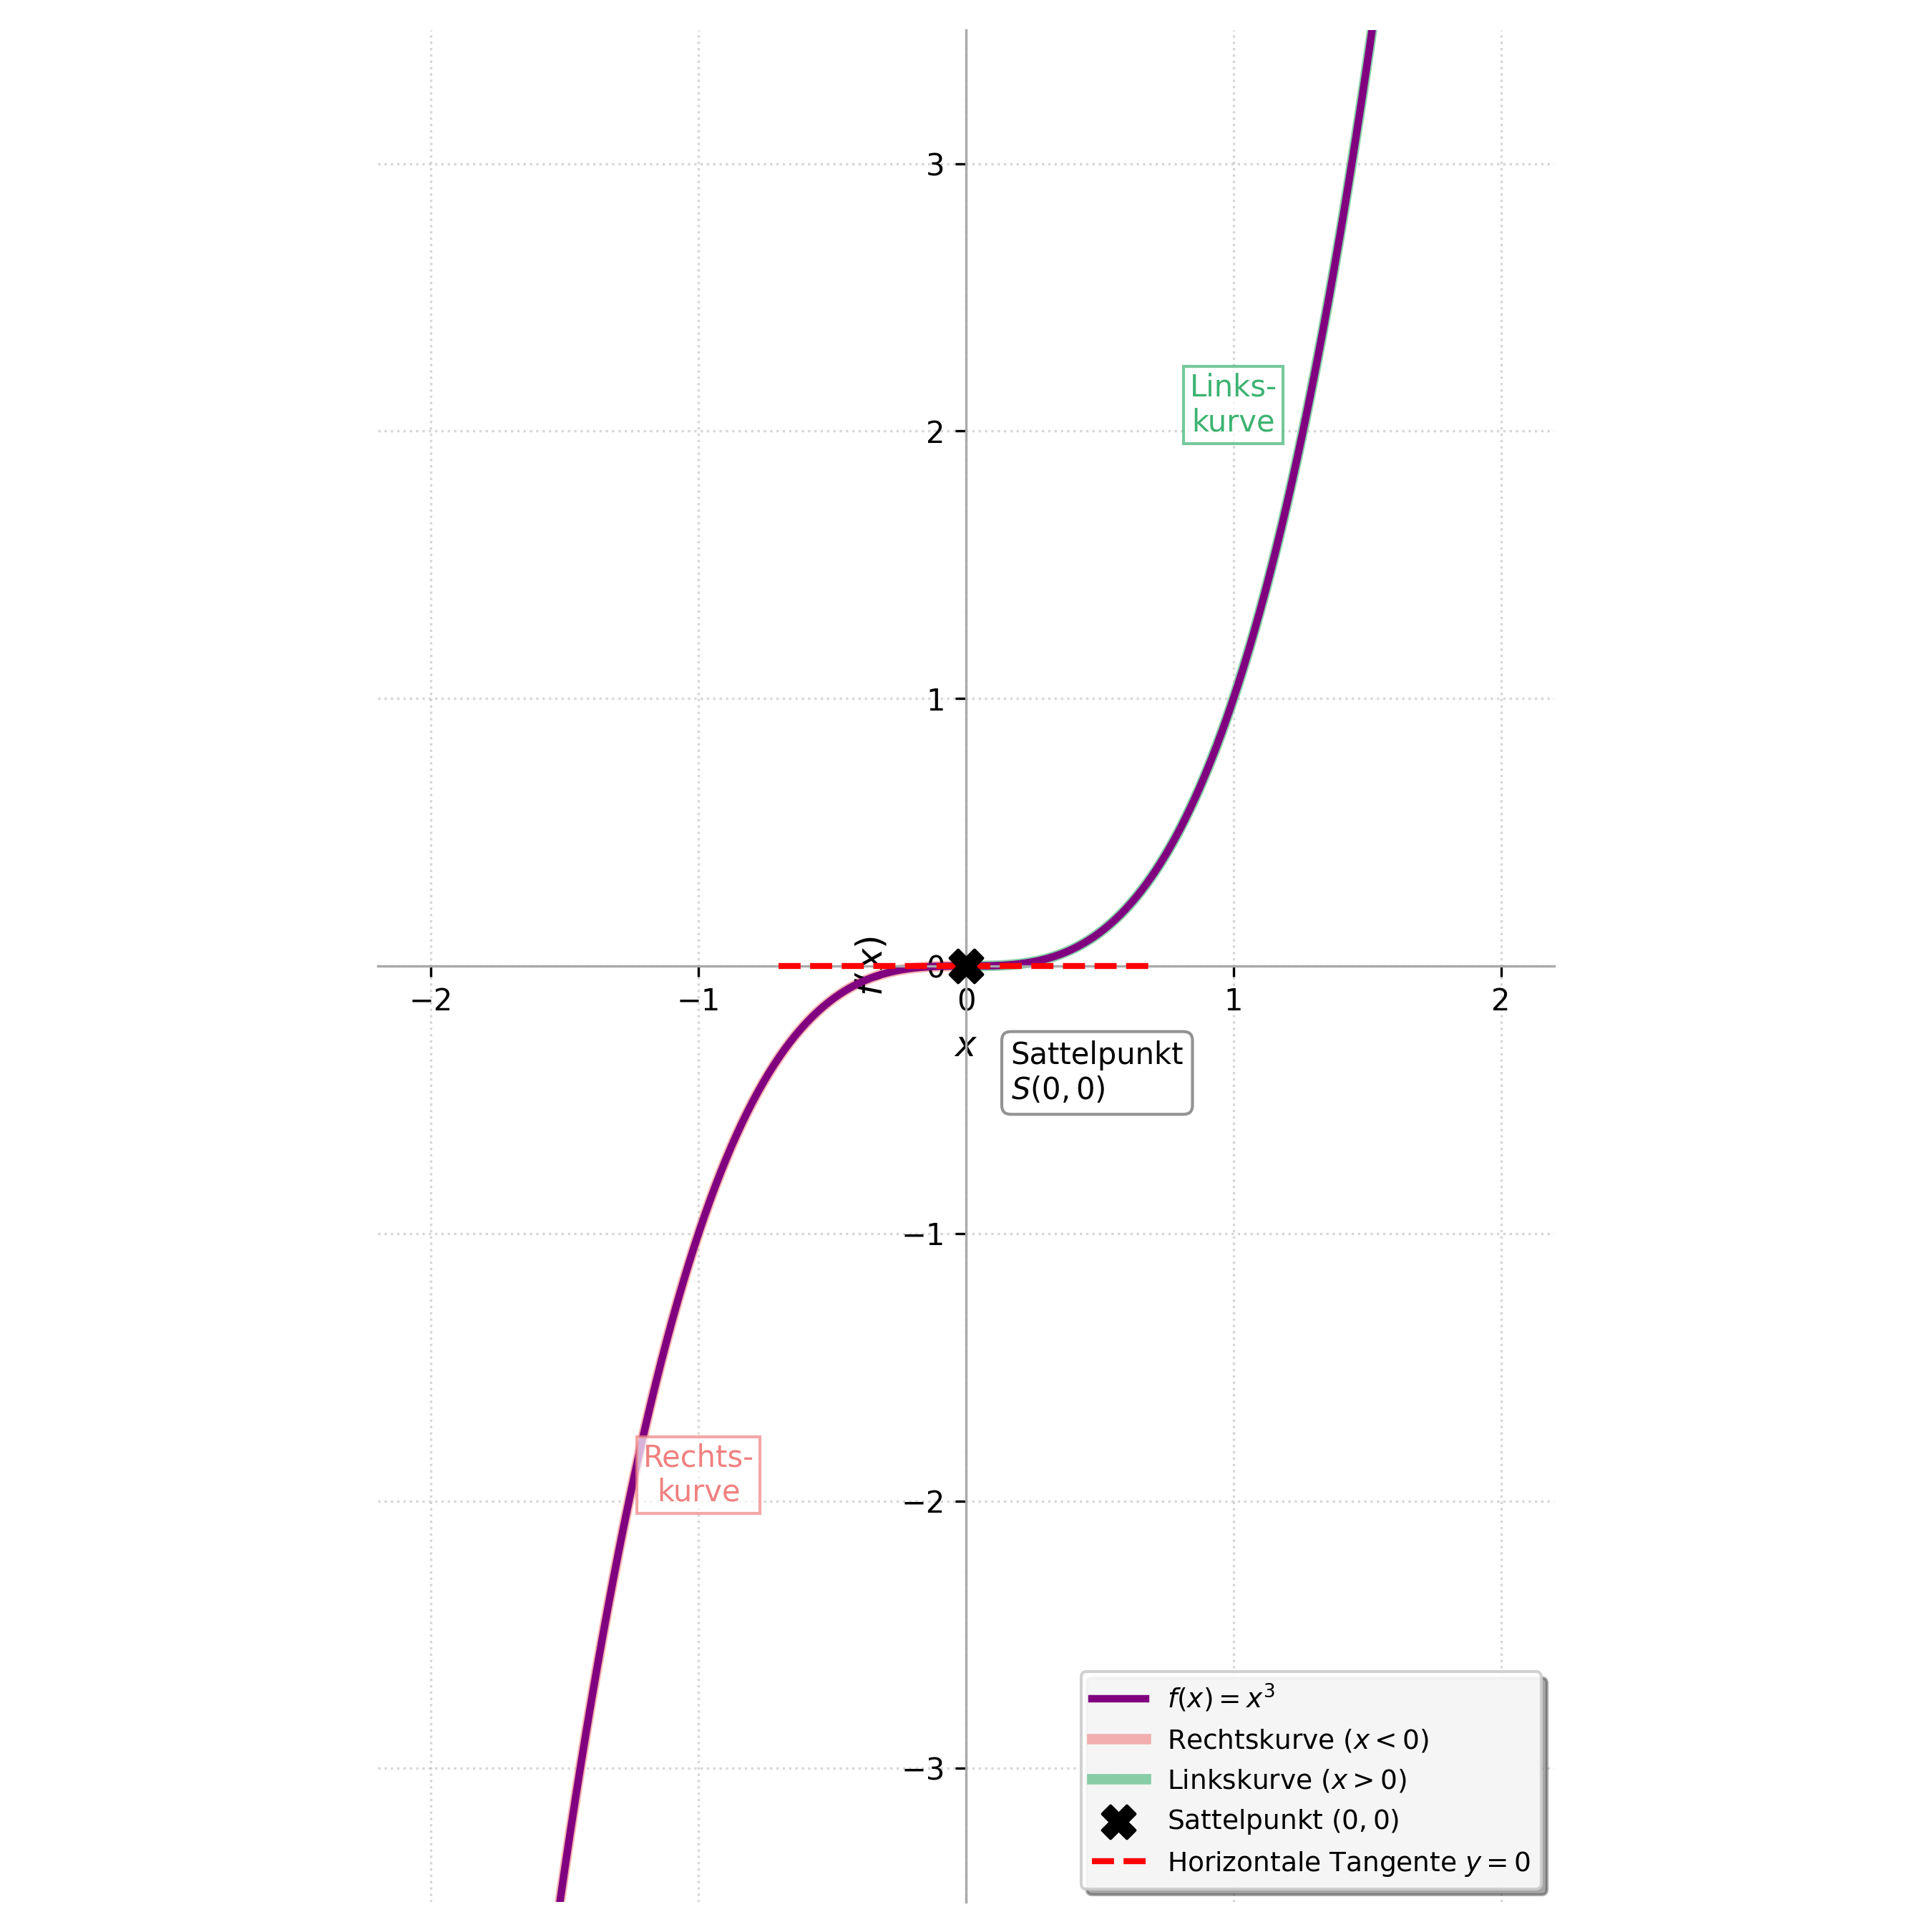
\includegraphics[width=0.7\textwidth]{grafiken/Sattelpunkt_xhoch3.png}
    \captionof{figure}{Sattelpunkt der Funktion $f(x)=x^3$ im Ursprung}
    \label{fig:sattelpunkt_x3}
\end{center}
\end{beispielumgebung}

\begin{beispielumgebung}{Untersuchung auf Sattelpunkte bei \texorpdfstring{$f(x) = (x-1)^3 + 2$}{f(x) = (x-1) hoch 3 + 2}}
\begin{enumerate}
    \item \textbf{Ableitungen bilden (Kettenregel!):}
        $f(x) = (x-1)^3 + 2$
        $f'(x) = 3(x-1)^2 \cdot 1 + 0 = 3(x-1)^2$
        $f''(x) = 3 \cdot 2(x-1)^1 \cdot 1 = 6(x-1)$
        $f'''(x) = 6$

    \item \textbf{Potentielle Stellen für horizontale Tangenten:}
        $f'(x) = 0 \implies 3(x-1)^2 = 0 \implies (x-1)^2 = 0 \implies x-1=0 \implies x = 1$.
        Kritische Stelle ist $x_S = 1$.

    \item \textbf{Überprüfung mit Vorzeichenwechsel von $f'(x)$:}
        $f'(x) = 3(x-1)^2$. Da $(x-1)^2$ immer $\ge 0$ ist (und nur für $x=1$ gleich Null ist), ist $f'(x) \ge 0$ für alle $x$.
        Es gibt keinen Vorzeichenwechsel bei $x=1$. Also kein Extrempunkt.

    \item \textbf{Überprüfung der Wendepunktbedingungen:}
        $f''(x_S) = f''(1) = 6(1-1) = 6 \cdot 0 = 0$. (Notwendige Bedingung erfüllt).
        $f'''(x_S) = f'''(1) = 6 \neq 0$. (Hinreichende Bedingung erfüllt).
        Da $f'(1)=0$ und bei $x=1$ ein Wendepunkt vorliegt, ist $P(1|f(1))$ ein Sattelpunkt.

    \item \textbf{Koordinaten des Sattelpunkts:}
        $f(1) = (1-1)^3 + 2 = 0^3 + 2 = 2$.
        Der Sattelpunkt ist $S(1|2)$.
\end{enumerate}
\end{beispielumgebung}

\begin{tippumgebung}{Systematisches Vorgehen bei der Suche nach Sattelpunkten}
\begin{enumerate}
    \item Berechne $f'(x)$ und $f''(x)$ (und ggf. $f'''(x)$).
    \item Setze $f'(x)=0$ und löse nach $x$. Das sind die Kandidaten $x_E$ für Extrem- oder Sattelpunkte.
    \item Setze diese Kandidaten $x_E$ in $f''(x)$ ein:
        \begin{itemize}
            \item Wenn $f''(x_E) \neq 0$, dann liegt ein Extrempunkt vor (Hochpunkt bei $f''(x_E)<0$, Tiefpunkt bei $f''(x_E)>0$).
            \item Wenn $f''(x_E) = 0$, dann könnte ein Sattelpunkt vorliegen. Fahre fort mit Schritt 4.
        \end{itemize}
    \item Wenn $f'(x_E)=0$ und $f''(x_E)=0$:
        \begin{itemize}
            \item Prüfe $f'''(x_E)$. Wenn $f'''(x_E) \neq 0$, dann ist es ein Sattelpunkt.
            \item Alternativ (oder wenn $f'''(x_E)$ auch $0$ ist): Prüfe das Vorzeichenwechselkriterium für $f'(x)$ an der Stelle $x_E$. Gibt es keinen Vorzeichenwechsel, ist es ein Sattelpunkt (vorausgesetzt, es ist auch ein Wendepunkt, d.h. $f''(x)$ wechselt an $x_E$ das Vorzeichen).
        \end{itemize}
\end{enumerate}
\end{tippumgebung}

\begin{aufgabenumgebung}{Extrempunkte und Sattelpunkte finden und identifizieren}
Untersuche die folgenden Funktionen auf Extrempunkte und Sattelpunkte. Gib jeweils die Koordinaten und die Art des Punktes an. Nutze die notwendigen und hinreichenden Bedingungen.

\begin{enumerate}
    \item $f(x) = x^3 - 3x^2 + 3x + 1$
        \begin{tippumgebung}{Analyse dieser kubischen Funktion}
        Bestimme $f'(x)$ und $f''(x)$. Gibt es Stellen $x_S$, für die $f'(x_S)=0$ und $f''(x_S)=0$ gilt? Überprüfe dann $f'''(x_S)$ oder das Vorzeichenwechselverhalten von $f'(x)$ an diesen Stellen. Hat die Funktion auch 'normale' Extrempunkte?
        \end{tippumgebung}

    \item $g(x) = \frac{1}{4}x^4 - \frac{1}{2}x^2 + 1$
        \begin{tippumgebung}{Polynom 4. Grades}
        Diese Funktion ähnelt einer der ursprünglichen Aufgaben. Untersuche hier sorgfältig alle kritischen Stellen ($g'(x)=0$). Prüfe, ob bei $g''(x_E)=0$ eventuell ein Sattelpunkt vorliegt oder ob es sich trotz $g''(x_E)=0$ um ein Extremum handeln könnte (dann das VZW-Kriterium für $g'(x)$ nutzen!). Hat diese Funktion Sattelpunkte?
        \end{tippumgebung}

    \item $h(x) = x^5 - \frac{5}{3}x^3$
        \begin{tippumgebung}{Ein Polynom 5. Grades}
        Bestimme $h'(x)$, $h''(x)$ und $h'''(x)$.
        \begin{itemize}
            \item Wo ist $h'(x)=0$?
            \item Welche dieser Stellen sind auch Nullstellen von $h''(x)$?
            \item Was sagt $h'''(x)$ an diesen speziellen Stellen aus? Gibt es sowohl Extrempunkte als auch Sattelpunkte?
        \end{itemize}
        \end{tippumgebung}

    \item \textbf{Für Experten:} Konstruiere eine Polynomfunktion $k(x)$ vom Grad 5, die bei $x=0$ einen Sattelpunkt hat und bei $x=2$ einen Tiefpunkt. (Beginne mit den Bedingungen für die Ableitungen.)
\end{enumerate}
\end{aufgabenumgebung}

\begin{fehlerboxumgebung}{Sattelpunkte nicht übersehen}
\begin{itemize}
    \item Wenn $f'(x_E)=0$ und $f''(x_E)=0$ ist, ist die Untersuchung noch nicht abgeschlossen! Es könnte ein Sattelpunkt sein. Man darf nicht vorschnell auf 'kein Extremum' schließen, ohne die Wendepunkteigenschaft (z.B. mit $f'''(x_E) \neq 0$ oder VZW von $f''$) zu prüfen.
    \item Ein Sattelpunkt ist ein Wendepunkt, aber nicht jeder Wendepunkt ist ein Sattelpunkt (nur die mit horizontaler Tangente).
\end{itemize}
\end{fehlerboxumgebung}

\begin{kurzknappumgebung}{Sattelpunkte}
\begin{itemize}
    \item \textbf{Definition:} Ein Punkt auf dem Graphen, an dem die Tangente waagerecht ist ($f'(x_S)=0$), aber kein Extremum vorliegt (kein Vorzeichenwechsel von $f'(x)$).
    \item \textbf{Eigenschaft:} Sattelpunkte sind immer auch Wendepunkte (Krümmungswechsel).
    \item \textbf{Bedingungen (üblich):} $f'(x_S)=0$ UND $f''(x_S)=0$ UND $f'''(x_S) \neq 0$.
\end{itemize}
\end{kurzknappumgebung}








\subsubsection{Nullstellen von Polynomen höheren Grades – Die Polynomdivision}
\label{subsubsec:polynomdivision}

Für quadratische Funktionen (Grad 2) haben wir die p-q-Formel oder die Mitternachtsformel, um Nullstellen zu finden. Aber was machen wir bei Polynomen höheren Grades, z.B. $f(x) = x^3 - 2x^2 - 5x + 6$? Hierfür gibt es keine allgemeine, einfache Lösungsformel wie bei quadratischen Gleichungen.

Ein wichtiges Werkzeug, um die Nullstellen solcher Polynome zu finden, ist die \textbf{Polynomdivision}. Die Idee ist, wenn wir eine Nullstelle $x_1$ des Polynoms $f(x)$ kennen (z.B. durch Raten oder aus dem Kontext der Aufgabe), dann wissen wir, dass $(x-x_1)$ ein Faktor von $f(x)$ sein muss.
Stell dir vor, du multiplizierst Linearfaktoren: $(x-x_1)(x-x_2)(x-x_3)$ würde ein Polynom 3. Grades ergeben, dessen Nullstellen $x_1, x_2, x_3$ sind. Die Polynomdivision ist der umgekehrte Prozess: Wir teilen das gegebene Polynom durch einen bekannten Faktor $(x-x_1)$, um ein Restpolynom zu erhalten, dessen Grad um 1 niedriger ist.

\begin{merksatzumgebung}{Polynomdivision}
Wenn $x_1$ eine Nullstelle eines Polynoms $f(x)$ vom Grad $n$ ist, dann ist der Term $(x-x_1)$ ein Linearfaktor von $f(x)$. Man kann $f(x)$ durch $(x-x_1)$ ohne Rest teilen:
\[ f(x) : (x-x_1) = g(x) \]
wobei $g(x)$ ein Restpolynom vom Grad $n-1$ ist. Die weiteren Nullstellen von $f(x)$ sind dann die Nullstellen von $g(x)$.
Wenn $f(x)$ vom Grad 3 ist, ist $g(x)$ vom Grad 2, und dessen Nullstellen können wir mit der p-q-Formel oder Mitternachtsformel finden.
\end{merksatzumgebung}

Das Verfahren der Polynomdivision ähnelt der schriftlichen Division von Zahlen.

\begin{beispielumgebung}{Polynomdivision durchführen}
Gegeben ist das Polynom $f(x) = x^3 - 2x^2 - 5x + 6$. Wir haben durch Probieren (z.B. Teiler des konstanten Gliedes 6: $\pm 1, \pm 2, \pm 3, \pm 6$) herausgefunden, dass $x_1=1$ eine Nullstelle ist, denn $f(1) = 1^3 - 2(1)^2 - 5(1) + 6 = 1 - 2 - 5 + 6 = 0$.
Wir teilen nun $f(x)$ durch den Linearfaktor $(x-1)$:
\[ (x^3 - 2x^2 - 5x + 6) : (x-1) \]

\polyset{style=C, vars=x, div=:} % Setzt den Divisionsoperator auf ':'
\polylongdiv{x^3 - 2x^2 - 5x + 6}{x-1}

Das Ergebnis der Polynomdivision ist $x^2 - x - 6$.
Nun suchen wir die Nullstellen dieses quadratischen Restpolynoms $g(x) = x^2 - x - 6$:
$x^2 - x - 6 = 0$. Mit der p-q-Formel ($p=-1, q=-6$):
$x_{2,3} = - \frac{-1}{2} \pm \sqrt{(\frac{-1}{2})^2 - (-6)} = \frac{1}{2} \pm \sqrt{\frac{1}{4} + \frac{24}{4}} = \frac{1}{2} \pm \sqrt{\frac{25}{4}} = \frac{1}{2} \pm \frac{5}{2}$.
$x_2 = \frac{1+5}{2} = \frac{6}{2} = 3$.
$x_3 = \frac{1-5}{2} = \frac{-4}{2} = -2$.
Die Nullstellen der Funktion $f(x) = x^3 - 2x^2 - 5x + 6$ sind also $x_1=1$, $x_2=3$ und $x_3=-2$.
\end{beispielumgebung}

\begin{tippumgebung}{Nullstelle raten und Koeffizientenvergleich}
Das Raten einer ersten Nullstelle (oft ganzzahlige Teiler des konstanten Gliedes) ist ein üblicher erster Schritt. Wenn die Polynomdivision zu aufwendig erscheint oder nicht explizit gefordert ist, kann man nach dem Finden einer Nullstelle $x_1$ auch den \textbf{Koeffizientenvergleich} nutzen, wie im Tipp der Aufgabe $s(x)$ in der nächsten Aufgabensammlung gezeigt.
\end{tippumgebung}
% --- ENDE DES NEUEN ABSCHNITTS ZUR POLYNOMDIVISION ---


\begin{aufgabenumgebung}{Nullstellen finden – Übung und Vertiefung}
Berechne die Nullstellen der folgenden Funktionen. Entscheide selbst, welche Methode (Ausklammern, p-q-Formel, Mitternachtsformel, Substitution, Polynomdivision nach Raten einer Nullstelle) am besten geeignet ist. Überprüfe bei quadratischen Gleichungen immer zuerst die Diskriminante, um die Anzahl der erwarteten reellen Nullstellen zu bestimmen.
\begin{enumerate}
    \item $f(x) = x^2 - x - 6$
        \begin{tippumgebung}{Lösungsweg}
        Dies ist eine Standard-quadratische Gleichung. p-q-Formel oder Mitternachtsformel sind hier gut geeignet.
        \end{tippumgebung}

    \item $g(x) = -2x^2 + 12x - 18$ 
        \begin{tippumgebung}{Besondere Diskriminante}
        Was sagt $D=0$ über den Graphen und die Art der Nullstelle aus?
        \end{tippumgebung}

    \item $h(x) = x^2 + 2x + 5$
        \begin{tippumgebung}{Keine reellen Nullstellen?}
        Was bedeutet es für den Graphen, wenn die Diskriminante $D<0$ ist?
        \end{tippumgebung}

    \item $k(x) = 3x^2 - 12$ 
        \begin{tippumgebung}{Vereinfachung}
        Hier geht es auch ohne Mitternachtsformel! Denke an das direkte Auflösen nach $x^2$. (Siehe Infobox zu Sonderfällen).
        \end{tippumgebung}

    \item $m(x) = -0.5x^2 + 2x$
        \begin{tippumgebung}{Ausklammern}
        Auch hier ist Ausklammern der schnellste Weg! (Siehe Infobox zu Sonderfällen).
        \end{tippumgebung}

    \item \textbf{Polynom 3. Grades durch Ausklammern:}
        $p(x) = x^3 - 5x^2 + 6x$
        \begin{tippumgebung}{Strategie}
        Klammere zuerst den gemeinsamen Faktor $x$ aus. Übrig bleibt ein quadratischer Term, dessen Nullstellen du mit den bekannten Formeln finden kannst.
        \end{tippumgebung}

    \item \textbf{Biquadratische Funktion:}
        $q(x) = x^4 - 10x^2 + 9$
        \begin{tippumgebung}{Substitution}
        Ersetze (substituiere) $x^2$ durch eine neue Variable, z.B. $z = x^2$. Dadurch erhältst du eine quadratische Gleichung in $z$. Löse diese nach $z$ und substituiere dann zurück ($x^2 = z_1$, $x^2 = z_2$), um die Nullstellen für $x$ zu finden. Achtung: Nicht jede Lösung für $z$ führt zu reellen Lösungen für $x$!
        \end{tippumgebung}

    \item \textbf{Produkt aus Linearfaktoren (versteckt):}
        $r(x) = (x^2-4)(x^2+x-2)$
        \begin{tippumgebung}{Satz vom Nullprodukt und Faktorisieren}
        Ein Produkt ist Null, wenn einer der Faktoren Null ist. Setze also jeden Klammerausdruck gleich Null. Der erste Faktor lässt sich mit der 3. binomischen Formel zerlegen. Für den zweiten Faktor kannst du die p-q-Formel verwenden.
        \end{tippumgebung}

    \item \textbf{Funktion mit bekannter Nullstelle (Polynomdivision anwenden):}
        Gegeben ist die Funktion $s(x) = x^3 - 2x^2 - 5x + 6$. Es ist bekannt, dass $x_1=1$ eine Nullstelle ist. Finde die anderen Nullstellen mithilfe der Polynomdivision.
        \textit{(Vergleiche auch den Tipp mit dem Koeffizientenvergleich aus der vorherigen Version dieser Aufgabe.)}

    \item \textbf{Nullstellen und Parameter:}
        Für welche Werte des Parameters $k$ hat die Funktion $f_k(x) = x^2 - 2kx + (k+2)$ genau eine, zwei oder keine reelle(n) Nullstelle(n)?
        \begin{tippumgebung}{Diskriminante}
        Untersuche die Diskriminante $D = b^2-4ac$ der quadratischen Gleichung $f_k(x)=0$ in Abhängigkeit von $k$.
        Setze $D=0$ für eine Nullstelle, $D>0$ für zwei und $D<0$ für keine.
        \end{tippumgebung}
    \item \textbf{Anwendung des Satzes von Vieta (Kopfrechnen für Profis):}
        Versuche, die Nullstellen der folgenden quadratischen Funktionen (in Normalform $x^2+px+q=0$) durch 'scharfes Hinsehen' mit dem Satz von Vieta zu finden. Suche also zwei Zahlen $x_1, x_2$, für die gilt: $x_1+x_2 = -p$ und $x_1 \cdot x_2 = q$.
        \begin{enumerate}[label=(\alph*)]
            \item $f(x) = x^2 - 5x + 6$
            \item $g(x) = x^2 + 2x - 8$
            \item $h(x) = x^2 - 7x + 10$
        \end{enumerate}
        \begin{tippumgebung}{Satz von Vieta nutzen}
        Für $f(x) = x^2 - 5x + 6$: Hier ist $p=-5$ und $q=6$. Du suchst also zwei Zahlen, deren Summe $-p = -(-5) = 5$ ist und deren Produkt $q=6$ ist. Welche Zahlen könnten das sein? (Denke an die Teiler von 6).
        \end{tippumgebung}
\end{enumerate}
\end{aufgabenumgebung}





\subsection{Kurvendiskussion von Polynomfunktionen – Das Gesamtpaket}
\label{subsec:kurvendiskussion_polynome}

Mit unserem Wissen über Ableitungen und Grenzwerte können wir nun eine vollständige Kurvendiskussion für Polynomfunktionen durchführen. Das Ziel ist es, ein umfassendes Bild vom Verlauf des Graphen zu erhalten, ohne jeden einzelnen Punkt berechnen zu müssen.

\begin{merksatzumgebung}{Checkliste für die Kurvendiskussion eines Polynoms}
Für eine Polynomfunktion $f(x) = a_n x^n + \dots + a_0$ untersuchen wir typischerweise:
\begin{enumerate}
    \item \textbf{Definitionsbereich ($D_f$):} Für Polynome immer $D_f = \mathbb{R}$.
    \item \textbf{Symmetrie:}
        \begin{itemize}
            \item \textbf{Achsensymmetrie zur y-Achse?}: Gilt $f(-x) = f(x)$? (Tritt auf, wenn $f(x)$ nur gerade Exponenten von $x$ enthält, z.B. $f(x)=x^4-2x^2+1$).
            \item \textbf{Punktsymmetrie zum Ursprung?}: Gilt $f(-x) = -f(x)$? (Tritt auf, wenn $f(x)$ nur ungerade Exponenten von $x$ enthält, z.B. $f(x)=x^3-x$).
            \item Ansonsten ist keine einfache Symmetrie zum Koordinatensystem vorhanden (aber ggf. zu einem anderen Punkt oder einer anderen Achse, was hier seltener untersucht wird).
        \end{itemize}
    \item \textbf{Verhalten im Unendlichen (Grenzwerte):} $\lim_{x \to \pm \infty} f(x)$ (siehe Abschnitt \ref{subsec:grenzwerte}).
    \item \textbf{Schnittpunkt mit der y-Achse ($P_y$):} Berechne $f(0)$. Der Punkt ist $P_y(0|f(0))$. (Bei Polynomen ist $f(0)=a_0$, der konstante Term).
    \item \textbf{Nullstellen ($N_i$):} Setze $f(x)=0$ und löse die Gleichung.
        \begin{itemize}
            \item Bei Grad $n=2$: p-q-Formel oder Mitternachtsformel.
            \item Bei Grad $n>2$:
                \begin{itemize}
                    \item $x$ ausklammern, falls kein konstanter Term $a_0$ vorhanden ist ($a_0=0$).
                    \item Eine Nullstelle $x_1$ raten (oft $\pm 1, \pm 2, \dots$, Teiler von $a_0$) und dann Polynomdivision durch $(x-x_1)$ durchführen, um den Grad zu reduzieren. \textit{Hinweis: Polynomdivision wird in diesem Skript nicht explizit behandelt. Aufgaben werden so gestellt, dass sie ohne lösbar sind, z.B. durch Ausklammern oder Substitution.}
                    \item Bei biquadratischen Gleichungen (z.B. $ax^4+bx^2+c=0$): Substitution $z=x^2$ verwenden.
                \end{itemize}
        \end{itemize}
    \item \textbf{Erste Ableitung $f'(x)$ bilden.}
    \item \textbf{Extremstellen (Hoch-/Tiefpunkte):}
        \begin{itemize}
            \item Notwendige Bedingung: $f'(x_E)=0$. Lösungen sind potentielle Extremstellen $x_E$.
            \item Hinreichende Bedingung: Vorzeichenwechsel von $f'(x)$ an $x_E$ ODER $f''(x_E) \neq 0$.
                \begin{itemize}
                    \item $f'(x)$ VZW von $+$ nach $-$ ODER $f''(x_E) < 0 \implies$ Hochpunkt.
                    \item $f'(x)$ VZW von $-$ nach $+$ ODER $f''(x_E) > 0 \implies$ Tiefpunkt.
                \end{itemize}
            \item y-Koordinaten: $y_E = f(x_E)$. Punkte $H(x_E|y_E)$ oder $T(x_E|y_E)$.
        \end{itemize}
    \item \textbf{Monotonieverhalten:} Intervalle bestimmen, in denen $f'(x)>0$ (steigend) oder $f'(x)<0$ (fallend).
    \item \textbf{Zweite Ableitung $f''(x)$ bilden.}
    \item \textbf{Wendepunkte ($W$):}
        \begin{itemize}
            \item Notwendige Bedingung: $f''(x_W)=0$. Lösungen sind potentielle Wendestellen $x_W$.
            \item Hinreichende Bedingung: Vorzeichenwechsel von $f''(x)$ an $x_W$ ODER $f'''(x_W) \neq 0$.
            \item y-Koordinaten: $y_W = f(x_W)$. Punkt $W(x_W|y_W)$.
        \end{itemize}
    \item \textbf{Krümmungsverhalten:} Intervalle bestimmen, in denen $f''(x)>0$ (linksgekrümmt) oder $f''(x)<0$ (rechtsgekrümmt).
    \item \textbf{Wertetabelle (optional):} Für wichtige Punkte und zur Verfeinerung der Skizze.
    \item \textbf{Skizze des Graphen:} Alle berechneten Punkte und Informationen verwenden.
\end{enumerate}
\end{merksatzumgebung}

\begin{beispielumgebung}[Kurvendiskussion Polynom 3. Grades]{Untersuchung von $f(x) = \frac{1}{3}x^3 - x^2 - 3x$}
\begin{enumerate}
    \item \textbf{Definitionsbereich:} $D_f = \mathbb{R}$.
    \item \textbf{Symmetrie:}
        $f(-x) = \frac{1}{3}(-x)^3 - (-x)^2 - 3(-x) = -\frac{1}{3}x^3 - x^2 + 3x$.
        $f(-x) \neq f(x)$ und $f(-x) \neq -f(x)$. Keine einfache Symmetrie zum Koordinatensystem.
    \item \textbf{Verhalten im Unendlichen:} Höchste Potenz ist $\frac{1}{3}x^3$ ($n=3$ ungerade, $a_3=\frac{1}{3}>0$).
        $\lim_{x \to \infty} f(x) = +\infty$; $\lim_{x \to -\infty} f(x) = -\infty$. (Kommt von links unten, geht nach rechts oben).
    \item \textbf{y-Achsenabschnitt:} $f(0) = \frac{1}{3}(0)^3 - (0)^2 - 3(0) = 0$. Also $P_y(0|0)$.
    \item \textbf{Nullstellen:} $f(x)=0 \implies \frac{1}{3}x^3 - x^2 - 3x = 0$.
        Wir können $x$ ausklammern: $x(\frac{1}{3}x^2 - x - 3) = 0$.
        Eine Nullstelle ist $x_1 = 0$.
        Für die anderen lösen wir $\frac{1}{3}x^2 - x - 3 = 0$. Multiplizieren mit 3: $x^2 - 3x - 9 = 0$.
        p-q-Formel ($p=-3, q=-9$):
        $x_{2,3} = - \frac{-3}{2} \pm \sqrt{(\frac{-3}{2})^2 - (-9)} = \frac{3}{2} \pm \sqrt{\frac{9}{4} + \frac{36}{4}} = \frac{3}{2} \pm \sqrt{\frac{45}{4}} = \frac{3}{2} \pm \frac{\sqrt{45}}{2} = \frac{3 \pm \sqrt{9 \cdot 5}}{2} = \frac{3 \pm 3\sqrt{5}}{2}$.
        $x_2 = \frac{3 + 3\sqrt{5}}{2} \approx \frac{3 + 3 \cdot 2.236}{2} \approx \frac{3+6.708}{2} \approx \frac{9.708}{2} \approx 4.85$.
        $x_3 = \frac{3 - 3\sqrt{5}}{2} \approx \frac{3 - 6.708}{2} \approx \frac{-3.708}{2} \approx -1.85$.
        Nullstellen: $N_1(0|0)$, $N_2(\frac{3+3\sqrt{5}}{2}|0)$, $N_3(\frac{3-3\sqrt{5}}{2}|0)$.
    \item \textbf{Erste Ableitung:} $f'(x) = x^2 - 2x - 3$.
    \item \textbf{Extremstellen:} $f'(x)=0 \implies x^2 - 2x - 3 = 0$.
        p-q-Formel ($p=-2, q=-3$):
        $x_{E1,E2} = - \frac{-2}{2} \pm \sqrt{(\frac{-2}{2})^2 - (-3)} = 1 \pm \sqrt{1+3} = 1 \pm \sqrt{4} = 1 \pm 2$.
        $x_{E1} = 1+2 = 3$.
        $x_{E2} = 1-2 = -1$.
        Potentielle Extremstellen bei $x_{E_1}=3$ und $x_{E_2}=-1$.
    \item \textbf{Zweite Ableitung:} $f''(x) = (x^2 - 2x - 3)' = 2x - 2$.
    \item \textbf{Art der Extremstellen mit $f''$ prüfen:}
        $f''(3) = 2(3) - 2 = 6-2=4 > 0 \implies$ Tiefpunkt bei $x=3$.
        $y_T = f(3) = \frac{1}{3}(3)^3 - (3)^2 - 3(3) = 9 - 9 - 9 = -9$. Tiefpunkt $T(3|-9)$.
        $f''(-1) = 2(-1) - 2 = -2-2=-4 < 0 \implies$ Hochpunkt bei $x=-1$.
        $y_H = f(-1) = \frac{1}{3}(-1)^3 - (-1)^2 - 3(-1) = -\frac{1}{3} - 1 + 3 = -\frac{1}{3} + 2 = \frac{5}{3}$. Hochpunkt $H(-1|\frac{5}{3})$.
    \item \textbf{Monotonie:} Bestimmt durch Vorzeichen von $f'(x)=(x-3)(x+1)$.
        \begin{itemize}
            \item $x < -1$ (z.B. $x=-2$): $f'(-2)=(-)(-)=+ \implies$ steigend.
            \item $-1 < x < 3$ (z.B. $x=0$): $f'(0)=(+)(-)=- \implies$ fallend.
            \item $x > 3$ (z.B. $x=4$): $f'(4)=(+)(+)=+ \implies$ steigend.
        \end{itemize}
    \item \textbf{Wendepunkte:} $f''(x_W)=0 \implies 2x_W - 2 = 0 \implies 2x_W=2 \implies x_W=1$.
        Dritte Ableitung: $f'''(x) = (2x-2)' = 2$.
        $f'''(1) = 2 \neq 0 \implies$ Wendepunkt bei $x_W=1$.
        $y_W = f(1) = \frac{1}{3}(1)^3 - (1)^2 - 3(1) = \frac{1}{3} - 1 - 3 = \frac{1}{3} - 4 = -\frac{11}{3}$.
        Wendepunkt $W(1|-\frac{11}{3})$.
    \item \textbf{Krümmungsverhalten:} Bestimmt durch Vorzeichen von $f''(x)=2x-2$.
        \begin{itemize}
            \item $x < 1$: $f''(x) < 0 \implies$ rechtsgekrümmt.
            \item $x > 1$: $f''(x) > 0 \implies$ linksgekrümmt.
        \end{itemize}
    \item \textbf{Skizze:}
\begin{center}
    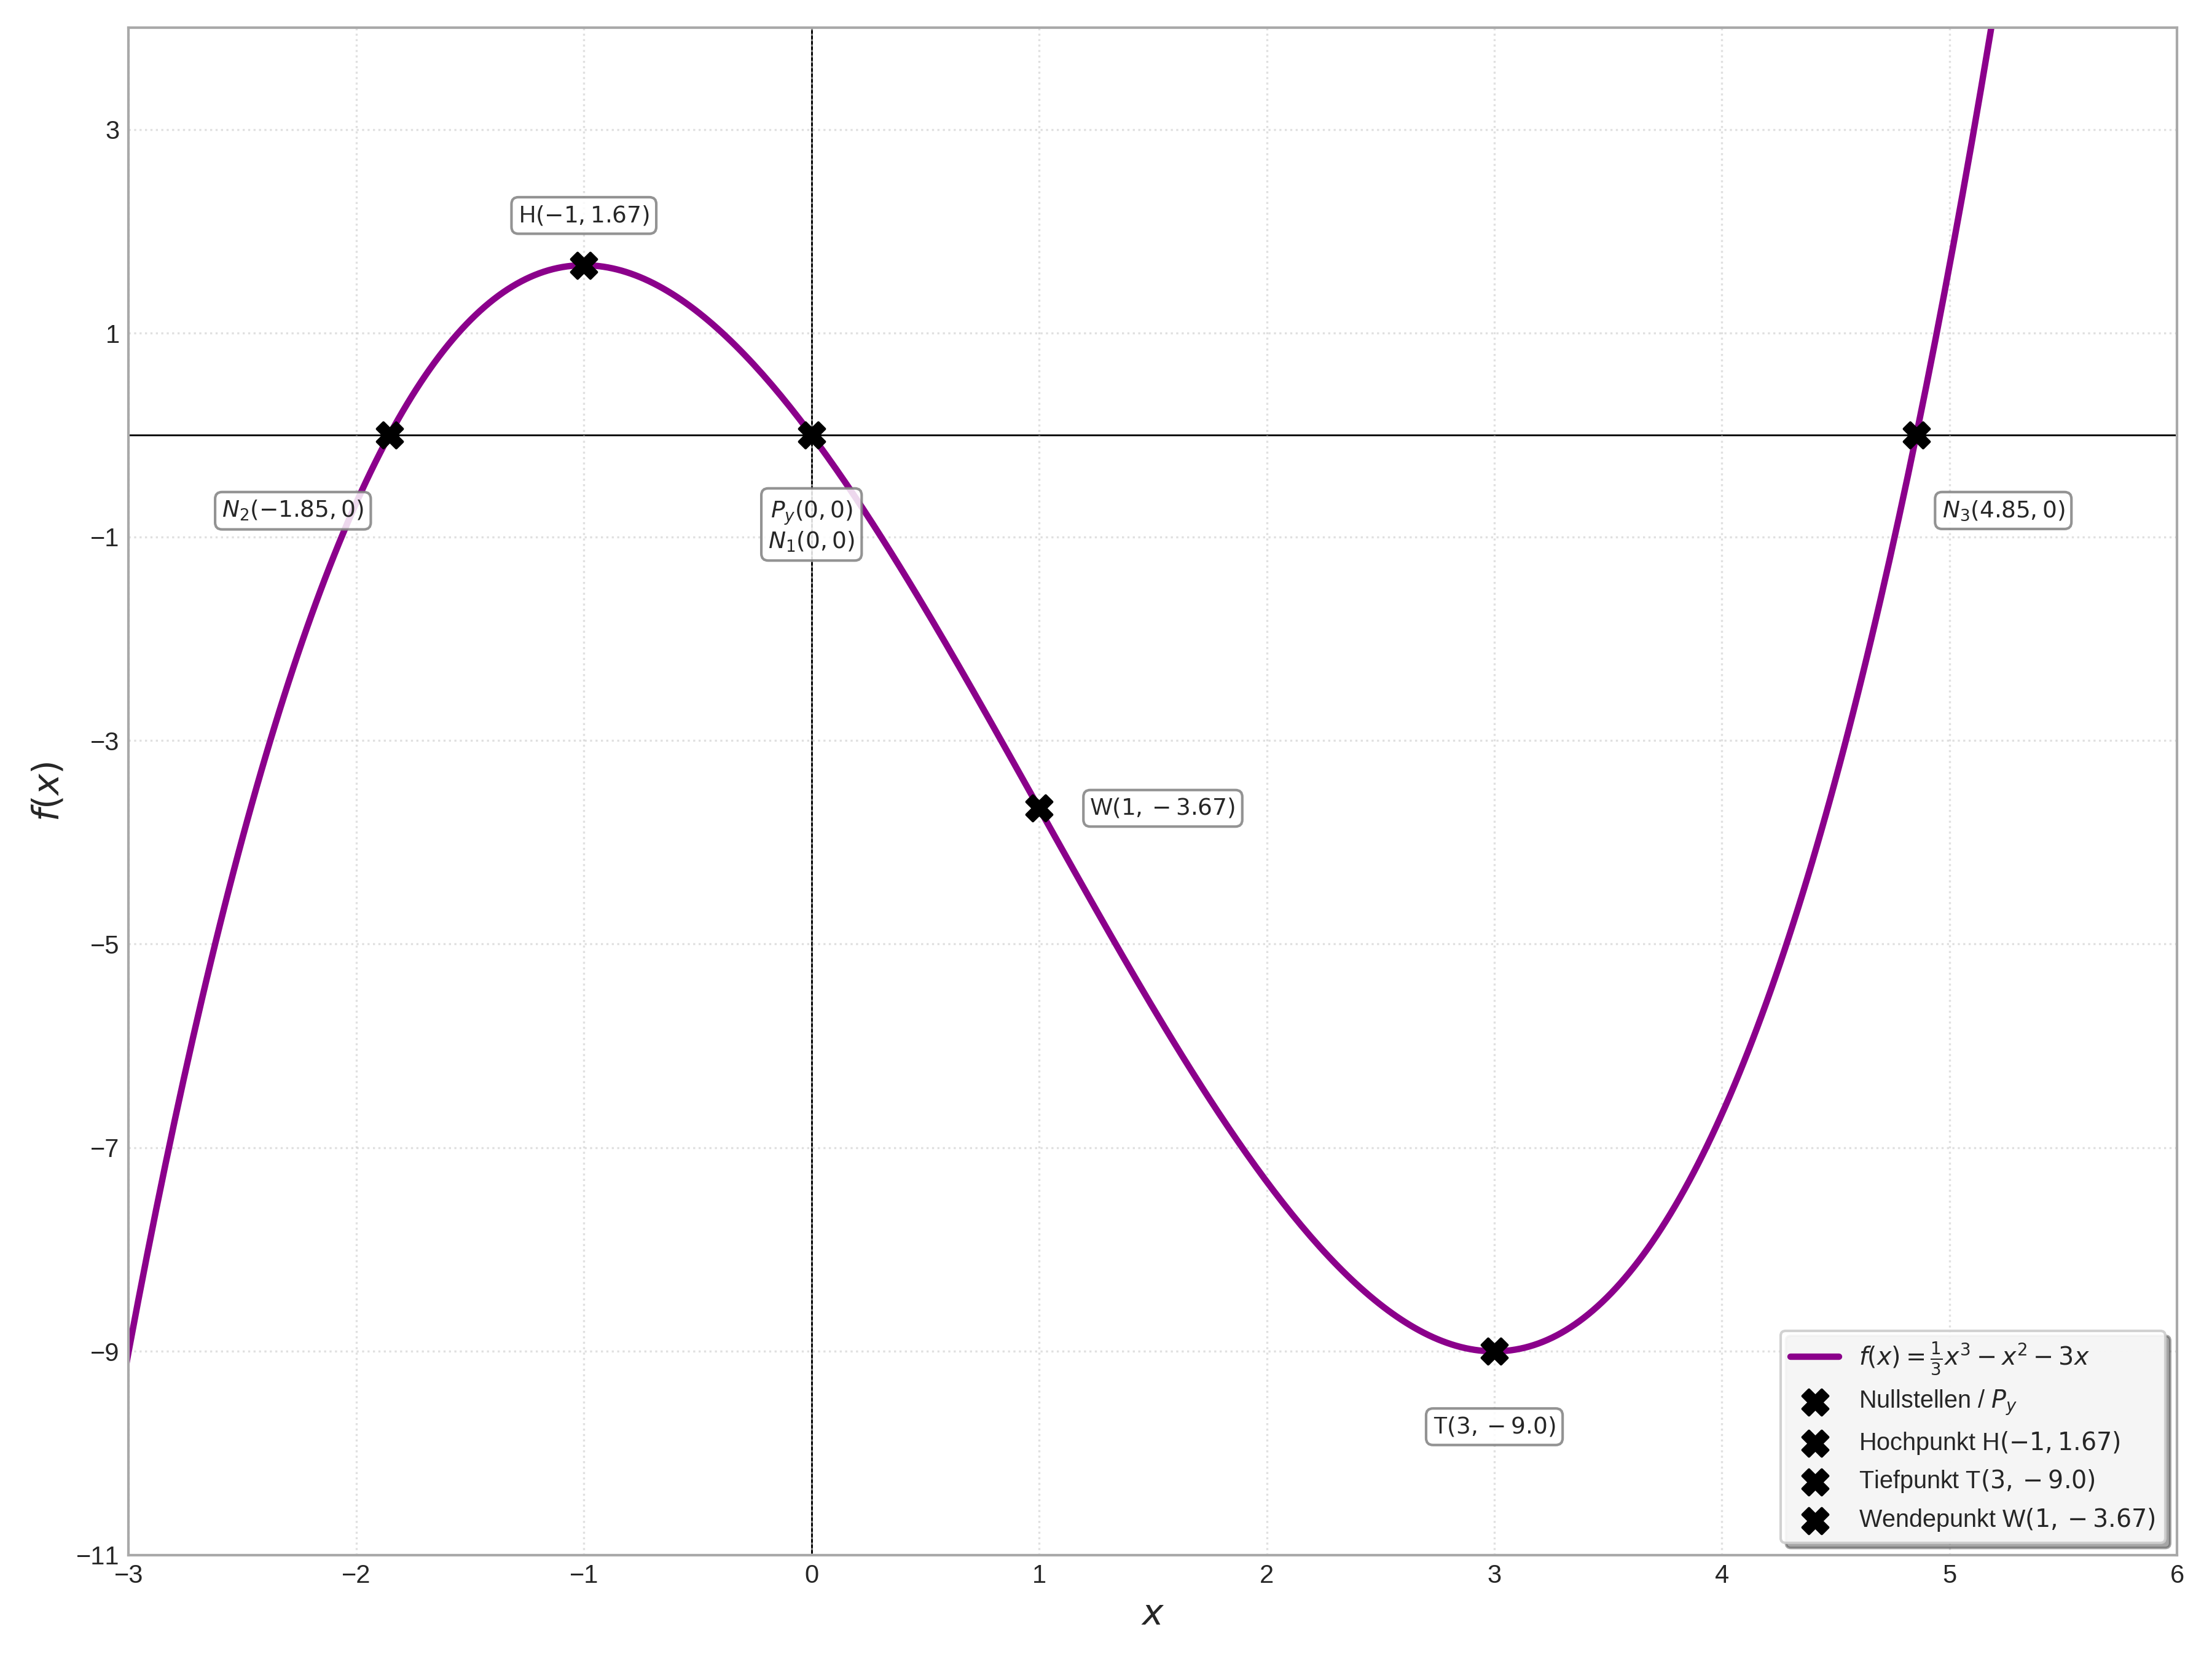
\includegraphics[width=0.9\textwidth]{grafiken/Kurvendiskussion_Polynom3.png}
    \captionof{figure}{Graph von $f(x) = \frac{1}{3}x^3 - x^2 - 3x$}
    \label{fig:kurvendisk_poly3}
\end{center}
\end{enumerate}
\end{beispielumgebung}

\begin{aufgabenumgebung}{Kurvendiskussionen von Polynomen}
Führe eine vollständige Kurvendiskussion (alle Punkte der Checkliste) für die folgenden Funktionen durch und skizziere jeweils den Graphen.
\begin{enumerate}
    \item \textbf{Quadratische Funktion als Wiederholung:} $f(x) = -x^2 + 4x - 3$. Vergleiche den gefundenen Extrempunkt mit dem Scheitelpunkt, den du mit der Formel $x_S = -b/(2a)$ oder quadratischer Ergänzung bestimmen kannst.
    \item \textbf{Kubische Funktion (einfache Nullstellen):} $g(x) = x^3 - 4x$. (Tipp: $x$ ausklammern für Nullstellen).
    \item \textbf{Biquadratische Funktion:} $h(x) = x^4 - 5x^2 + 4$. (Tipp für Nullstellen: Substituiere $z=x^2$, löse die quadratische Gleichung für $z$ und substituiere dann zurück. Beachte, dass diese Funktion achsensymmetrisch zur y-Achse ist!)
    \item \textbf{Für Experten (Polynom 3. Grades mit Raten):} $k(x) = x^3 - 7x - 6$. (Tipp: Eine ganzzahlige Nullstelle ist ein Teiler des konstanten Gliedes -6. Probiere $\pm 1, \pm 2, \pm 3, \pm 6$. Wenn du eine Nullstelle $x_1$ gefunden hast, kannst du den Term $(x-x_1)$ durch Polynomdivision (hier nicht erklärt, aber in Schulbüchern zu finden) oder durch einen anderen Trick (Koeffizientenvergleich) abspalten, um eine quadratische Restgleichung zu erhalten. Alternativ: Wenn du später die Produktregel kennst, kannst du versuchen, die Funktion geschickt zu faktorisieren, falls möglich, oder du nutzt einen Taschenrechner/Software, um die Nullstellen numerisch zu finden und konzentrierst dich auf die anderen Aspekte der Kurvendiskussion.)
        \item \textbf{Bewegung eines Objekts (Anwendung):}
        Die Höhe $h$ (in Metern) eines senkrecht nach oben geworfenen Steins nach $t$ Sekunden wird durch die Funktion $h(t) = -5t^2 + 20t + 1$ beschrieben (für $t \ge 0$ und solange $h(t) \ge 0$).
        \begin{enumerate}
            \item Bestimme die Geschwindigkeit $v(t) = h'(t)$ und die Beschleunigung $a(t) = h''(t)$ des Steins.
            \item Zu welchen Zeiten ist die Geschwindigkeit positiv (Stein steigt), negativ (Stein fällt) oder Null? Interpretiere diese Ergebnisse im Kontext der Bewegung.
            \item Wann erreicht der Stein seine maximale Höhe und wie hoch ist diese? (Tipp: Extrempunkt von $h(t)$)
            \item Wann kehrt der Stein zum Boden zurück (Annahme $h(t) \ge 0$)? (Tipp: Nullstelle von $h(t)$)
            \item Mit welcher Geschwindigkeit trifft der Stein auf dem Boden auf?
        \end{enumerate}
\end{enumerate}
\end{aufgabenumgebung}

\subsubsection{Nullstellen aus faktorisierter Form – Der Satz vom Nullprodukt}
\label{subsec:nullprodukt}

Manchmal liegen Polynomfunktionen bereits in einer \textbf{faktorisierten Form} vor, oder sie lassen sich leicht in eine solche überführen (z.B. durch Ausklammern). Diese Form ist besonders praktisch, um die Nullstellen direkt abzulesen. Das Zauberwort hierfür ist der \textbf{Satz vom Nullprodukt}.

\begin{merksatzumgebung}{Satz vom Nullprodukt}
Ein Produkt ist genau dann Null, wenn mindestens einer seiner Faktoren Null ist.
\[ A \cdot B = 0 \quad \Leftrightarrow \quad A=0 \text{ oder } B=0 \]
Das gilt natürlich auch für Produkte mit mehr als zwei Faktoren: $A \cdot B \cdot C = 0 \Leftrightarrow A=0 \text{ oder } B=0 \text{ oder } C=0$.
\end{merksatzumgebung}

Wenn eine Polynomfunktion in der Form $f(x) = k \cdot (x-x_1) \cdot (x-x_2) \cdot \dots \cdot (x-x_n)$ gegeben ist (wobei $k$ ein konstanter Faktor ist und $x_1, x_2, \dots, x_n$ die sogenannten Linearfaktoren sind), dann sind die Nullstellen der Funktion genau die Werte $x_1, x_2, \dots, x_n$. Denn wenn $x$ einen dieser Werte annimmt, wird einer der Klammerausdrücke Null, und damit das gesamte Produkt.

\begin{beispielumgebung}{Nullstellen aus faktorisierter Form ablesen}
\begin{enumerate}
    \item $f(x) = 2(x-1)(x+3)(x-5)$
    Die Funktion wird Null, wenn:
    \begin{itemize}
        \item $x-1=0 \implies x_1 = 1$
        \item $x+3=0 \implies x_2 = -3$
        \item $x-5=0 \implies x_3 = 5$
    \end{itemize}
    Die Nullstellen sind also $1, -3$ und $5$.

    \item $g(x) = -0.5x(x-2)^2(x+1)$
    Die Funktion wird Null, wenn:
    \begin{itemize}
        \item $x=0 \implies x_1 = 0$
        \item $(x-2)^2=0 \implies x-2=0 \implies x_2 = 2$ (Dies ist eine \textbf{doppelte Nullstelle}, da der Faktor $(x-2)$ zweimal vorkommt. An einer doppelten Nullstelle berührt der Graph die x-Achse, ohne sie zu schneiden.)
        \item $x+1=0 \implies x_3 = -1$
    \end{itemize}
    Die Nullstellen sind $0, 2$ (doppelt) und $-1$.

    \item $h(x) = x^3 - 4x$
    Hier müssen wir zuerst faktorisieren, indem wir $x$ ausklammern:
    $h(x) = x(x^2-4)$
    Den Term $x^2-4$ können wir mit der dritten binomischen Formel weiter faktorisieren: $x^2-4 = (x-2)(x+2)$.
    Also: $h(x) = x(x-2)(x+2)$.
    Die Nullstellen sind $x_1=0, x_2=2, x_3=-2$.
\end{enumerate}
\end{beispielumgebung}

\begin{aufgabenumgebung}{Nullstellen aus faktorisierter Form bestimmen}
Bestimme die Nullstellen der folgenden Funktionen. Gib auch an, ob es sich um einfache oder mehrfache Nullstellen handelt. Eine Kurvendiskussion zu diesen Funktionen kann natürlich auch nie schaden.
\begin{enumerate}
    \item $f(x) = (x+4)(x-2.5)(x+1)$
    \item $g(x) = -3x^2(x-1)(x+2)^3$
    \item $h(x) = (x^2-9)(x+1)$ (Tipp: $x^2-9$ weiter faktorisieren!)
    \item $k(x) = 2x^4 - 8x^2$ (Tipp: Erst ausklammern, dann weiter überlegen.)
\end{enumerate}
\end{aufgabenumgebung}

\begin{warumwichtigumgebung}{Faktorisierte Form und Nullstellen}
Die faktorisierte Form einer Polynomfunktion ist extrem nützlich, weil sie uns die Nullstellen quasi 'auf dem Silbertablett serviert'. Bei Kurvendiskussionen ist die Bestimmung der Nullstellen oft ein wichtiger Schritt. Wenn eine Funktion bereits faktorisiert ist oder sich leicht faktorisieren lässt, erspart uns das oft das aufwendige Raten von Nullstellen und die Polynomdivision.
Außerdem gibt die Vielfachheit einer Nullstelle (einfach, doppelt, dreifach etc.) Auskunft über das Verhalten des Graphen an dieser Stelle (schneiden oder berühren der x-Achse).
\end{warumwichtigumgebung}

\begin{infoboxumgebung}{Anwendungen von Kurvendiskussionen}
Kurvendiskussionen sind nicht nur eine mathematische Übung. Sie sind entscheidend, um reale Prozesse zu verstehen und zu optimieren:
\begin{itemize}
    \item \textbf{Wirtschaft:} Gewinnmaximierung, Kostenminimierung (Extremwertaufgaben).
    \item \textbf{Technik:} Optimale Formen für Bauteile, Stabilitätsanalysen.
    \item \textbf{Naturwissenschaften:} Modellierung von Wachstumsprozessen, Zerfallsprozessen, Bewegungen. Die Stellen, an denen sich Änderungsraten ändern (Wendepunkte), können wichtige Übergänge in Systemen markieren.
\end{itemize}
Das Verständnis, wie sich Funktionen verhalten, ist ein Kernstück angewandter Mathematik.
\end{infoboxumgebung}

\subsection{Exkurs: Grenzwerte von Funktionen mit negativen Exponenten}
\label{subsec:grenzwerte_neg_exp}

Bisher haben wir uns Polynomfunktionen angesehen, die für alle reellen Zahlen definiert sind ($D_f = \mathbb{R}$). Es gibt aber auch wichtige Funktionen, die nicht überall definiert sind, insbesondere solche, bei denen $x$ im Nenner steht. Das sind die einfachsten Formen von \textbf{gebrochen-rationalen Funktionen}. Ein typisches Beispiel ist $f(x) = \frac{1}{x}$ oder allgemeiner $f(x) = \frac{a}{x^n} = ax^{-n}$ mit $n > 0$.

Für diese Funktionen ist die Stelle $x=0$ besonders interessant. Wenn wir $x=0$ in den Nenner einsetzen würden, würde dieser Null werden, und \textbf{durch Null darf man nicht teilen}! Das bedeutet, die Funktion ist an der Stelle $x=0$ nicht definiert. Man sagt, die Funktion hat an der Stelle $x=0$ eine \textbf{Definitionslücke}. Der Definitionsbereich solcher Funktionen ist also $D_f = \mathbb{R} \setminus \{0\}$ (alle reellen Zahlen außer der Null). Wir untersuchen nun das Verhalten der Funktion, wenn sich $x$ dieser Lücke nähert.

\begin{merksatzumgebung}{Verhalten von $f(x) = \frac{a}{x^n}$ für $x \to 0$ (Polstellen)}
Wir betrachten Funktionen der Form $f(x) = \frac{a}{x^n}$ (oder $ax^{-n}$), wobei $a \neq 0$ eine Konstante ist und $n$ eine positive ganze Zahl ($n=1, 2, 3, \dots$).
Wie bereits erwähnt, ist $x=0$ nicht im Definitionsbereich dieser Funktionen. Diese spezielle Art von Definitionslücke, bei der die Funktionswerte gegen Unendlich ($+\infty$ oder $-\infty$) streben, wenn sich $x$ der Lücke nähert, nennt man eine \textbf{Polstelle} (oder kurz Pol).
Der Graph der Funktion hat an einer Polstelle eine \textbf{senkrechte Asymptote}. Für $f(x) = \frac{a}{x^n}$ ist dies die y-Achse (mit der Gleichung $x=0$). Eine Asymptote ist eine Gerade, der sich der Graph der Funktion beliebig annähert, sie aber nie erreicht oder schneidet.

Das Verhalten der Funktionswerte $f(x)$, wenn $x$ sich der Polstelle $x=0$ nähert, hängt davon ab, ob der Exponent $n$ im Nenner gerade oder ungerade ist und vom Vorzeichen des Zählers $a$:

\textbf{Fall 1: $n$ ist ungerade} (z.B. $f(x) = \frac{a}{x}$, $f(x) = \frac{a}{x^3}$)
Die Potenz $x^n$ behält das Vorzeichen von $x$.
\begin{itemize}
    \item Wenn $a > 0$:
        \begin{itemize}
            \item $\lim_{x \to 0^+} f(x) = +\infty$ (nähert man sich der 0 von rechts (positive $x$-Werte), wird $x^n$ positiv und klein $\implies \frac{a}{x^n}$ wird sehr groß positiv)
            \item $\lim_{x \to 0^-} f(x) = -\infty$ (nähert man sich der 0 von links (negative $x$-Werte), wird $x^n$ negativ und klein $\implies \frac{a}{x^n}$ wird sehr groß negativ)
        \end{itemize}
    \item Wenn $a < 0$: (Die Vorzeichen der Grenzwerte kehren sich um)
        \begin{itemize}
            \item $\lim_{x \to 0^+} f(x) = -\infty$
            \item $\lim_{x \to 0^-} f(x) = +\infty$
        \end{itemize}
\end{itemize}
Man spricht hier von einer \textbf{Polstelle mit Vorzeichenwechsel} (abgekürzt VZW). Der Graph 'springt' von $-\infty$ nach $+\infty$ (oder umgekehrt) an der Polstelle.

\textbf{Fall 2: $n$ ist gerade} (z.B. $f(x) = \frac{a}{x^2}$, $f(x) = \frac{a}{x^4}$)
Die Potenz $x^n$ ist immer positiv (oder Null), egal ob $x$ positiv oder negativ ist.
\begin{itemize}
    \item Wenn $a > 0$:
        \begin{itemize}
            \item $\lim_{x \to 0^+} f(x) = +\infty$ (nähert man sich der 0 von rechts, wird $x^n$ positiv und klein $\implies \frac{a}{x^n}$ wird sehr groß positiv)
            \item $\lim_{x \to 0^-} f(x) = +\infty$ (nähert man sich der 0 von links, wird $x^n$ ebenfalls positiv und klein $\implies \frac{a}{x^n}$ wird sehr groß positiv)
        \end{itemize}
    \item Wenn $a < 0$: (Die Vorzeichen der Grenzwerte kehren sich um)
        \begin{itemize}
            \item $\lim_{x \to 0^+} f(x) = -\infty$
            \item $\lim_{x \to 0^-} f(x) = -\infty$
        \end{itemize}
\end{itemize}
Man spricht hier von einer \textbf{Polstelle ohne Vorzeichenwechsel}. Der Graph geht auf beiden Seiten der Polstelle entweder nach $+\infty$ oder auf beiden Seiten nach $-\infty$.

Die Schreibweisen $x \to 0^+$ (lies: 'x geht von rechts gegen Null', d.h. $x$ nähert sich 0 mit Werten, die größer als 0 sind) und $x \to 0^-$ (lies: 'x geht von links gegen Null', d.h. $x$ nähert sich 0 mit Werten, die kleiner als 0 sind) bezeichnen die \textbf{einseitigen Grenzwerte}.
\end{merksatzumgebung}

\begin{beispielumgebung}{Grenzwerte an Polstellen}
\begin{enumerate}
    \item $f(x) = \frac{1}{x}$ ($a=1 > 0$, $n=1$ ungerade). Definitionsbereich $D_f = \mathbb{R} \setminus \{0\}$.
        \begin{itemize}
            \item $\lim_{x \to 0^+} \frac{1}{x} = +\infty$ (z.B. für $x=0.001$ ist $1/x = 1000$)
            \item $\lim_{x \to 0^-} \frac{1}{x} = -\infty$ (z.B. für $x=-0.001$ ist $1/x = -1000$)
        \end{itemize}
        Polstelle bei $x=0$ mit Vorzeichenwechsel.
        Symmetrie: $f(-x) = \frac{1}{-x} = -\frac{1}{x} = -f(x) \implies$ Punktsymmetrie zum Ursprung.

    \item $g(x) = \frac{-2}{x^2}$ ($a=-2 < 0$, $n=2$ gerade). Definitionsbereich $D_g = \mathbb{R} \setminus \{0\}$.
        \begin{itemize}
            \item $\lim_{x \to 0^+} \frac{-2}{x^2} = -\infty$ (z.B. für $x=0.01$ ist $x^2=0.0001$, $\frac{-2}{0.0001} = -20000$)
            \item $\lim_{x \to 0^-} \frac{-2}{x^2} = -\infty$ (z.B. für $x=-0.01$ ist $x^2=0.0001$, $\frac{-2}{0.0001} = -20000$)
        \end{itemize}
        Polstelle bei $x=0$ ohne Vorzeichenwechsel.
        Symmetrie: $g(-x) = \frac{-2}{(-x)^2} = \frac{-2}{x^2} = g(x) \implies$ Achsensymmetrie zur y-Achse.
\end{enumerate}
\begin{center}
    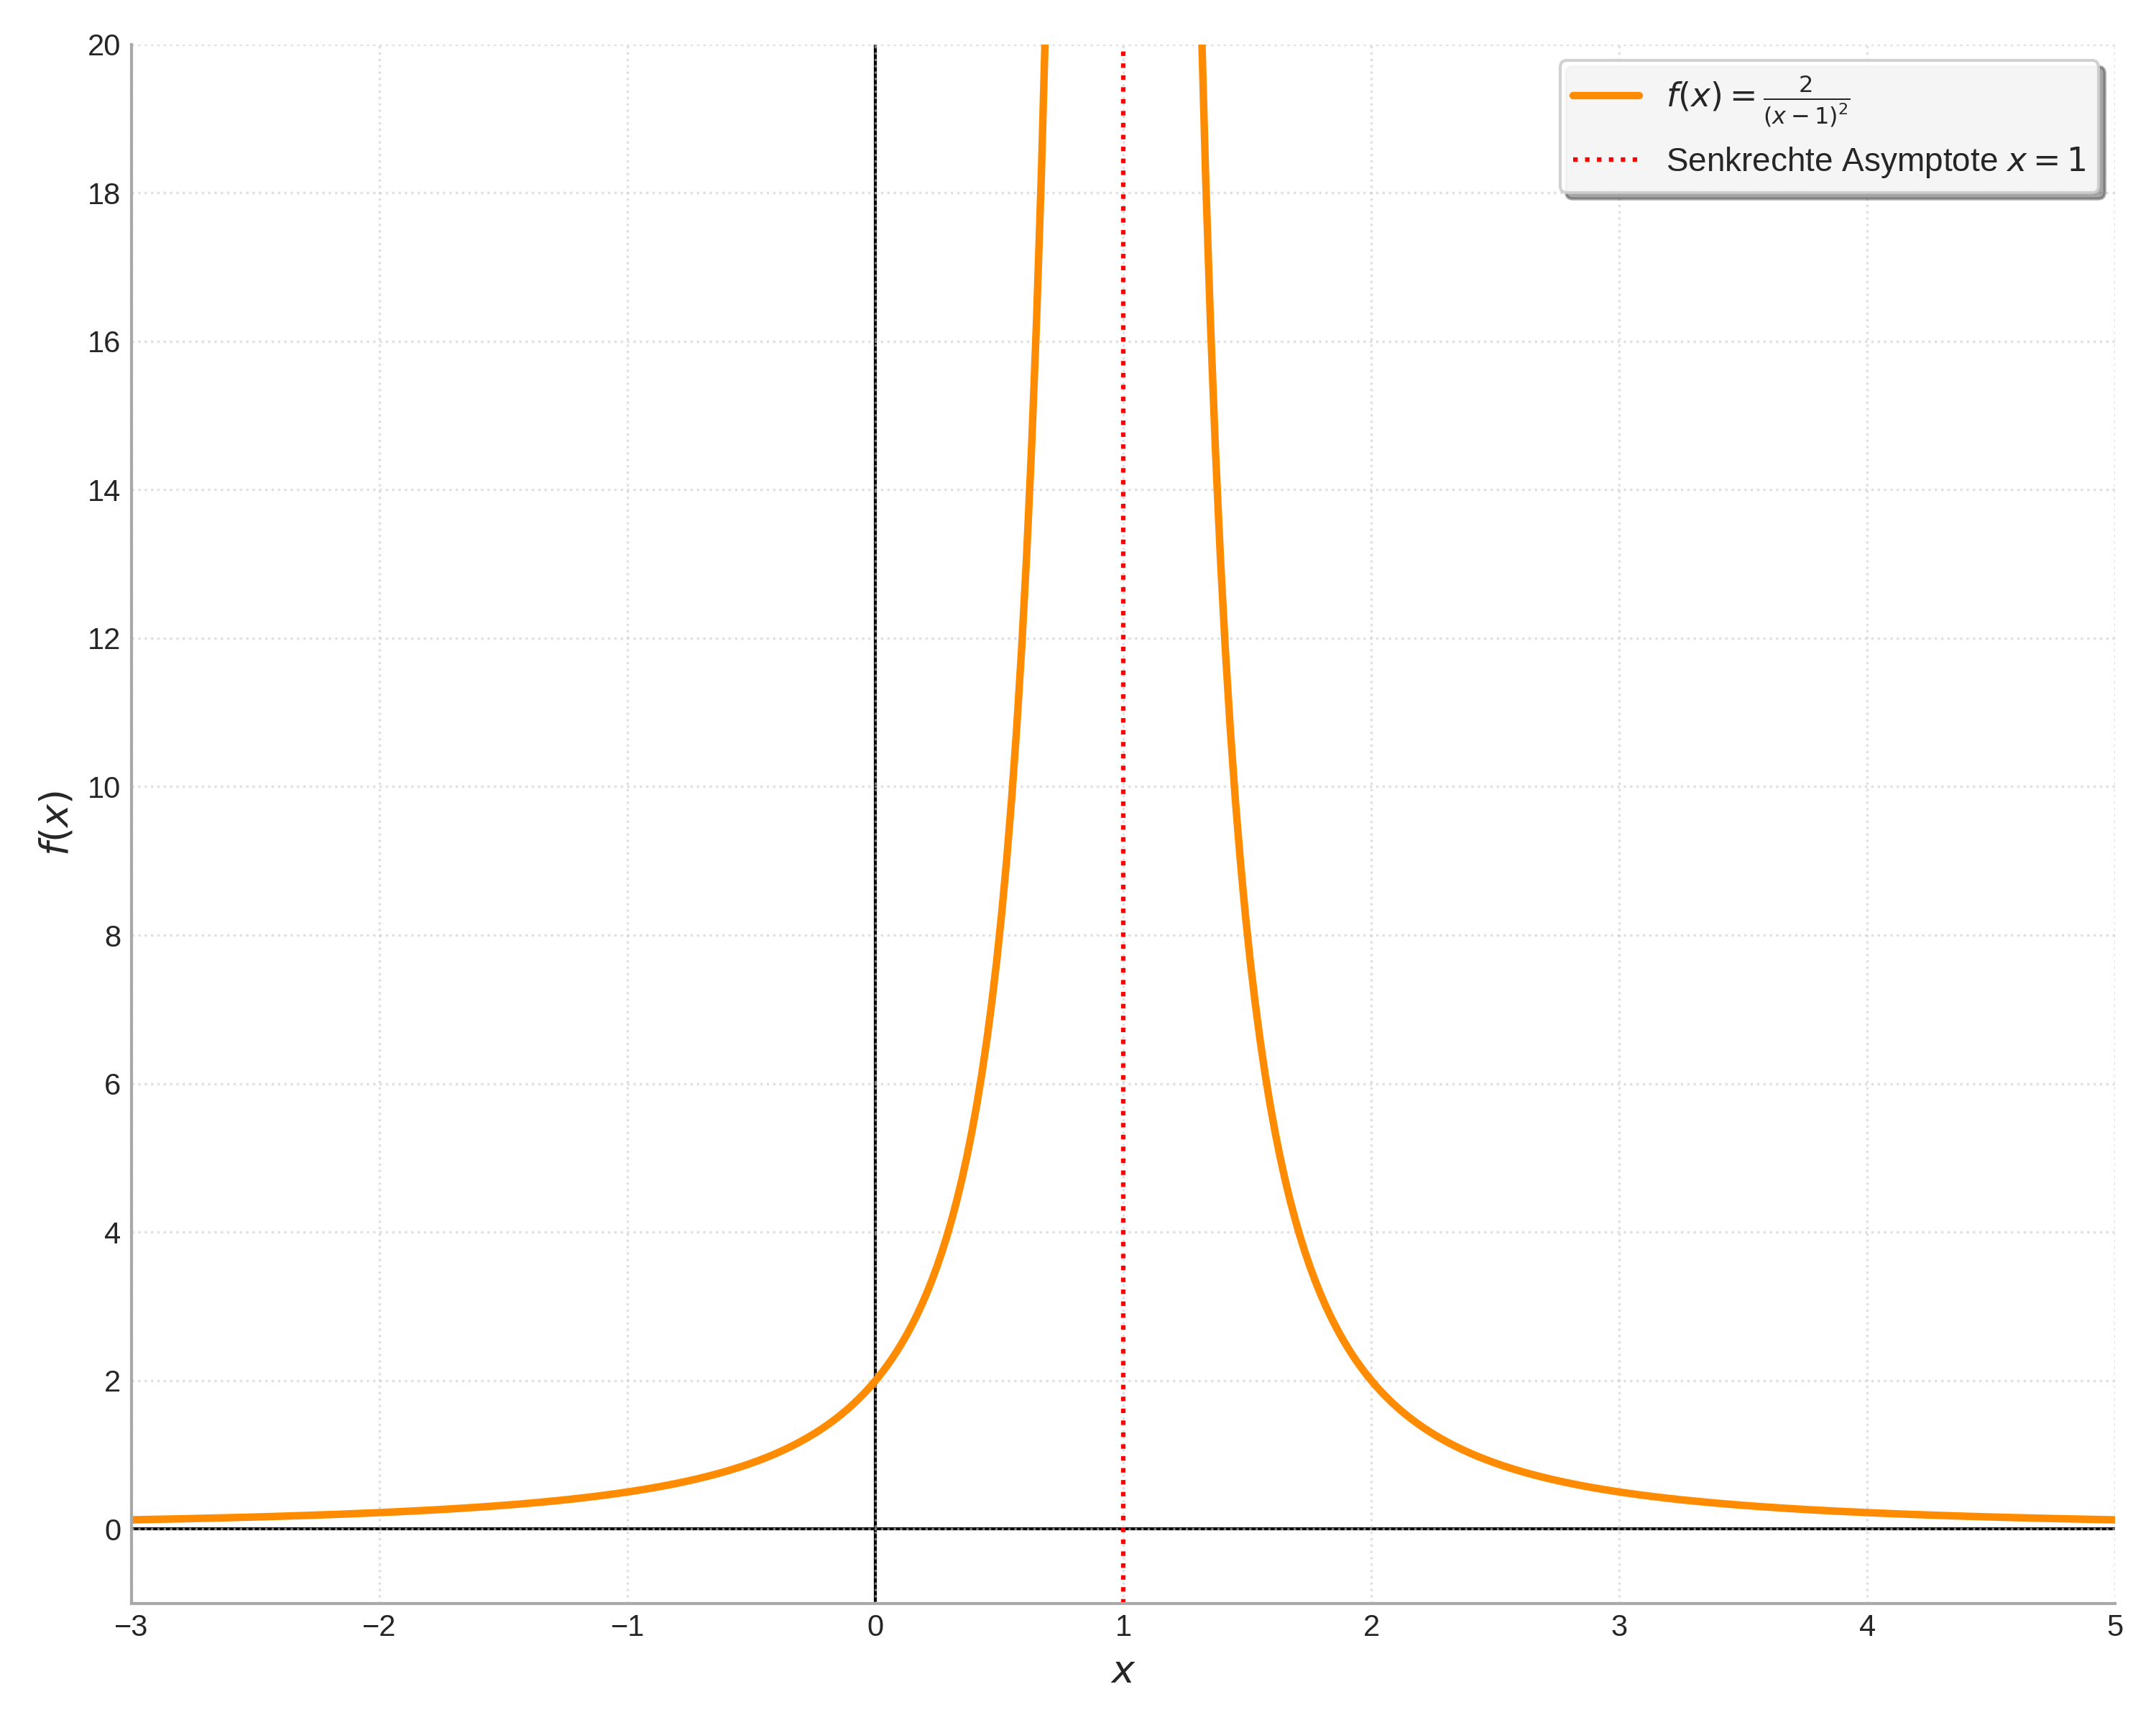
\includegraphics[width=0.8\textwidth]{grafiken/Gebrochen_Rational_Verschoben.png}
    \captionof{figure}{Graph von $f(x)=\frac{2}{(x-1)^2}$}
    \label{fig:gebr_rat_verschoben}
\end{center}
\end{beispielumgebung}

\begin{aufgabenumgebung}{Grenzwerte und Symmetrie gebrochen-rationaler Grundfunktionen}
\begin{enumerate}
    \item Bestimme den Definitionsbereich und das Verhalten für $x \to 0^+$ und $x \to 0^-$ für die folgenden Funktionen. Gib auch an, ob es sich um eine Polstelle mit oder ohne Vorzeichenwechsel handelt.
        \begin{itemize}
            \item $f_1(x) = \frac{3}{x^3}$
            \item $f_2(x) = -\frac{1}{x^4}$
            \item $f_3(x) = \frac{10}{x}$
        \end{itemize}
    \item Untersuche die Symmetrie der Funktionen aus Teilaufgabe 1 (Achsensymmetrie zur y-Achse oder Punktsymmetrie zum Ursprung).
    \item \textbf{Zuordnung Aufgabe:} Ordne den folgenden Funktionsgraphen $k_1(x) = \frac{1}{x^2}$, $k_2(x) = -\frac{1}{x}$, $k_3(x) = \frac{2}{x^3}$, $k_4(x) = \frac{1}{x^4}$ die passenden Funktionsgleichungen zu. Begründe deine Entscheidung anhand des Verhaltens an der Polstelle $x=0$ und der Symmetrie.
    \begin{center}
        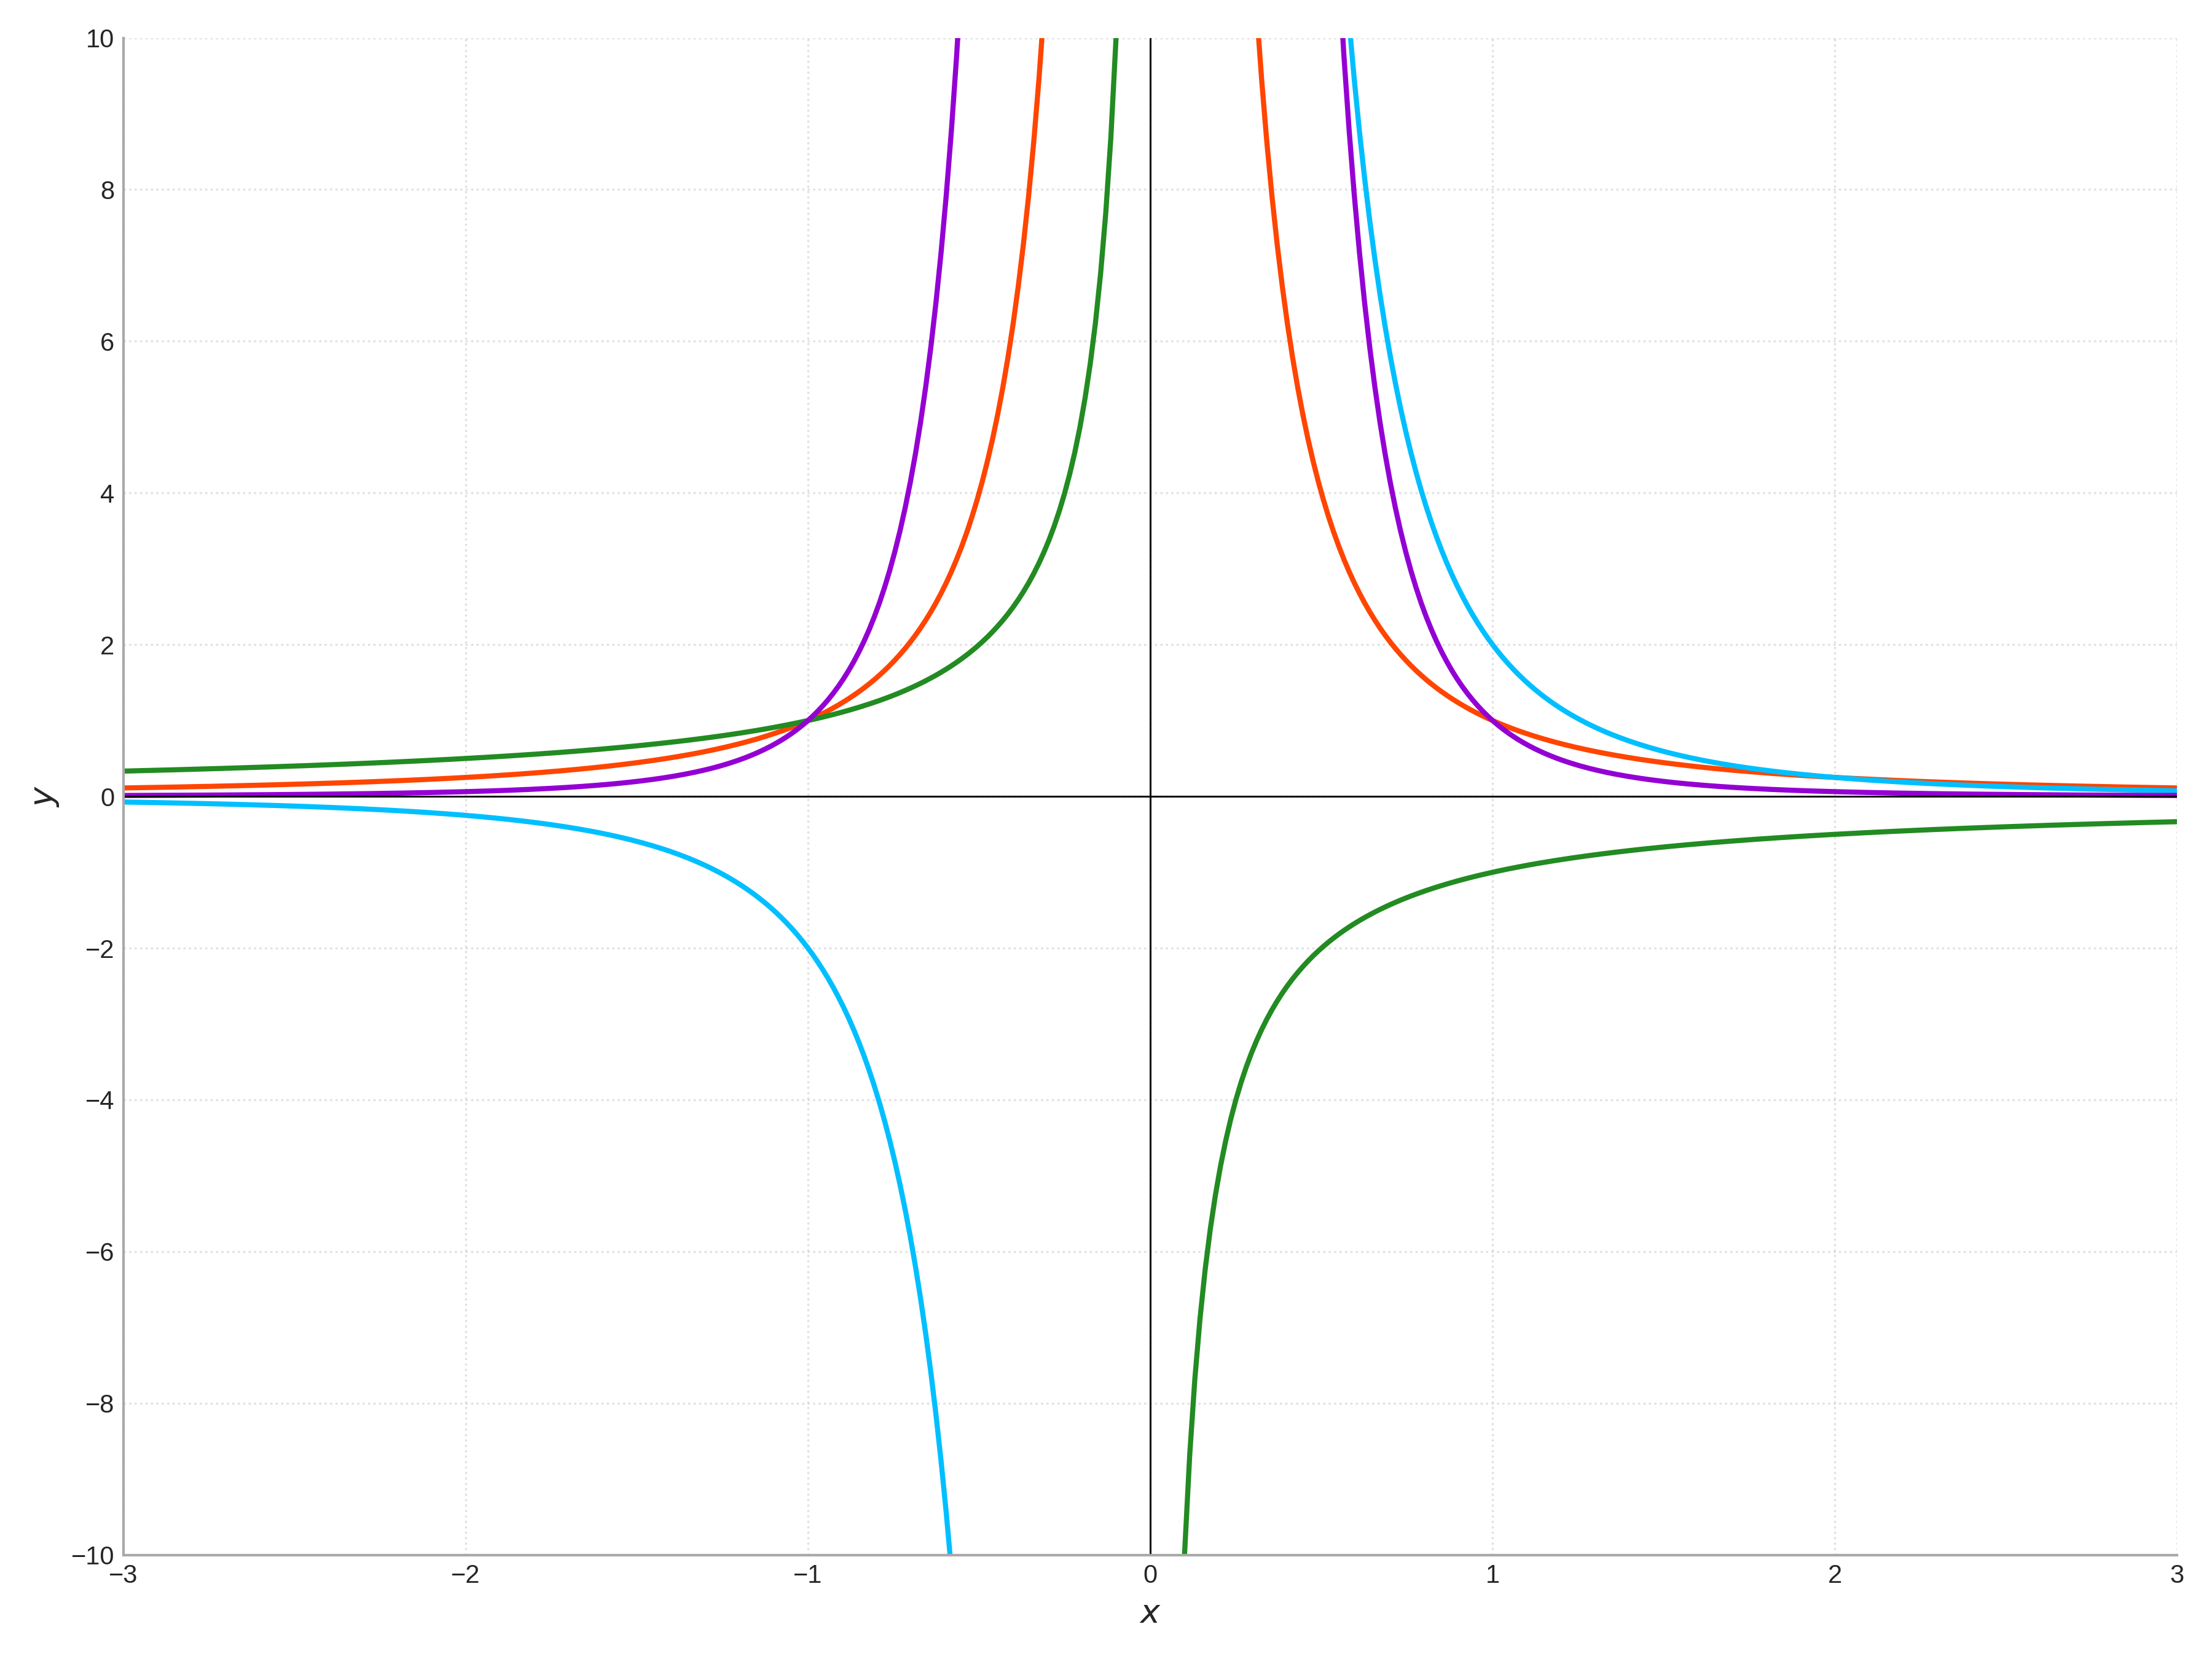
\includegraphics[width=0.9\textwidth]{grafiken/Zuordnung_Polstellen.png}
        \captionof{figure}{Graphen zur Zuordnung von Polstellenverhalten}
        \label{fig:zuordnung_polstellen}
    \end{center}
\end{enumerate}
\end{aufgabenumgebung}

Das Verständnis des Verhaltens von solchen Grundfunktionen an ihren Definitionslücken ist wichtig, da viele komplexere gebrochen-rationale Funktionen solche Terme enthalten.

\begin{kurzknappumgebung}{Verhalten an Polstellen ($f(x)=a/x^n$ bei $x=0$)}
\begin{itemize}
    \item \textbf{Definitionsbereich:} $D_f = \mathbb{R} \setminus \{0\}$ (Null ist nicht erlaubt, da man nicht durch Null teilen darf).
    \item \textbf{Polstelle:} Bei $x=0$ liegt eine Polstelle mit senkrechter Asymptote (y-Achse) vor.
    \item \textbf{Verhalten für $x \to 0$:}
        \begin{itemize}
            \item $n$ ungerade: Polstelle mit Vorzeichenwechsel (VZW). Die Funktionswerte gehen auf einer Seite gegen $+\infty$ und auf der anderen gegen $-\infty$. Das Vorzeichen von $a$ bestimmt, auf welcher Seite was passiert.
            \item $n$ gerade: Polstelle ohne Vorzeichenwechsel. Die Funktionswerte gehen auf beiden Seiten entweder gegen $+\infty$ (wenn $a>0$) oder gegen $-\infty$ (wenn $a<0$).
        \end{itemize}
    \item \textbf{Einseitige Grenzwerte} ($x \to 0^+$ und $x \to 0^-$) sind wichtig, um das Verhalten genau zu beschreiben.
\end{itemize}
\end{kurzknappumgebung}

\begin{fehlerboxumgebung}{Polstellen und Definitionsbereich}
\begin{itemize}
    \item \textbf{Definitionsbereich vergessen:} Immer zuerst den Definitionsbereich bestimmen! Eine Funktion kann nur dort Eigenschaften haben, wo sie auch definiert ist. Bei $f(x)=a/x^n$ ist $x=0$ \textbf{nicht} im Definitionsbereich.
    \item \textbf{Einseitige Grenzwerte verwechseln:} Achte genau darauf, ob du dich $x=0$ von positiven Werten ($x \to 0^+$) oder von negativen Werten ($x \to 0^-$) näherst, besonders bei ungeraden Exponenten $n$.
    \item \textbf{Vorzeichen von $a$ übersehen:} Das Vorzeichen von $a$ im Zähler kehrt die Richtung der 'Unendlichkeiten' um. Ist $a$ negativ, geht es z.B. bei $1/x^2$ nicht nach $+\infty$, sondern nach $-\infty$.
    \item \textbf{Polstelle mit Nullstelle verwechseln:} Eine Polstelle ist eine Definitionslücke, an der die Funktion 'explodiert'. Eine Nullstelle ist ein Punkt, an dem der Graph die x-Achse schneidet ($f(x)=0$). Funktionen wie $1/x$ haben keine Nullstellen.
\end{itemize}
\end{fehlerboxumgebung}

% HIER FOLGEN DANN DIE WEITEREN ABLEITUNGSREGELN (PRODUKT, QUOTIENT, KETTE)



% Vorheriger Inhalt des Kapitels bis zur Fehlerbox 'Polstellen und Definitionsbereich'
% ... (siehe vorherige Canvas-Version) ...

\subsubsection{Verhalten von $f(x) = \frac{a}{x^n}$ im Unendlichen und horizontale Asymptoten}

Wir haben das Verhalten von $f(x) = \frac{a}{x^n}$ in der Nähe der Polstelle $x=0$ untersucht. Aber was passiert, wenn $x$ sehr groß positiv ($x \to \infty$) oder sehr groß negativ ($x \to -\infty$) wird?

Wenn $n$ eine positive ganze Zahl ist ($n \ge 1$), dann wird der Nenner $x^n$ für betragsmäßig große $x$ sehr groß.
\begin{itemize}
    \item Für $x \to \infty$ wird $x^n \to \infty$.
    \item Für $x \to -\infty$:
        \begin{itemize}
            \item Wenn $n$ gerade ist, wird $x^n \to \infty$.
            \item Wenn $n$ ungerade ist, wird $x^n \to -\infty$.
        \end{itemize}
\end{itemize}
In allen diesen Fällen wird der Betrag von $x^n$ unendlich groß. Wenn wir nun eine feste Zahl $a$ durch eine unendlich große Zahl teilen, nähert sich das Ergebnis immer mehr der Null.

\begin{merksatzumgebung}{Grenzwert von $f(x) = \frac{a}{x^n}$ für $x \to \pm\infty$}
Für jede Funktion der Form $f(x) = \frac{a}{x^n}$ mit $a \neq 0$ und $n \in \mathbb{N}, n \ge 1$ gilt:
\[ \lim_{x \to \infty} \frac{a}{x^n} = 0 \]
\[ \lim_{x \to -\infty} \frac{a}{x^n} = 0 \]
Der Graph der Funktion nähert sich also für sehr große positive und sehr große negative $x$-Werte der x-Achse (der Geraden $y=0$) an. Man sagt, die Funktion hat eine \textbf{waagerechte (horizontale) Asymptote} bei $y=0$.
\end{merksatzumgebung}

\begin{beispielumgebung}{Horizontale Asymptoten}
\begin{enumerate}
    \item $f(x) = \frac{1}{x}$:
        $\lim_{x \to \infty} \frac{1}{x} = 0$ und $\lim_{x \to -\infty} \frac{1}{x} = 0$.
        Die x-Achse ($y=0$) ist eine waagerechte Asymptote.
        Zusammen mit der senkrechten Asymptote $x=0$ (y-Achse) ergibt sich das typische Bild einer Hyperbel.

    \item $g(x) = \frac{-2}{x^2}$:
        $\lim_{x \to \infty} \frac{-2}{x^2} = 0$ und $\lim_{x \to -\infty} \frac{-2}{x^2} = 0$.
        Auch hier ist die x-Achse ($y=0$) eine waagerechte Asymptote.
\end{enumerate}
\end{beispielumgebung}

\subsubsection{Substitution – Ein mächtiges Werkzeug zum Verständnis}

Manchmal sehen Funktionen komplizierter aus, als sie sind. Die Idee der \textbf{Substitution} (Ersetzung) kann uns helfen, bekannte Muster in neuen Verkleidungen zu erkennen.

Stell dir vor, du kennst das Verhalten der Funktion $f(x) = \frac{1}{x}$ sehr gut. Was ist dann mit der Funktion $g(x) = \frac{1}{x-5}$?
Wenn wir $z = x-5$ setzen (das ist unsere Substitution), dann ist $g(x)$ eigentlich $f(z) = \frac{1}{z}$. Die Funktion $g(x)$ verhält sich also genauso wie $f(x)$, nur dass alles um 5 Einheiten auf der x-Achse nach rechts verschoben ist!
\begin{itemize}
    \item $f(x) = \frac{1}{x}$ hat eine Polstelle bei $x=0$.
    \item $g(x) = \frac{1}{x-5}$ hat eine Polstelle dort, wo der Nenner Null wird, also bei $x-5=0 \implies x=5$.
\end{itemize}
Die senkrechte Asymptote verschiebt sich also von $x=0$ nach $x=5$. Das Verhalten um die Polstelle (mit Vorzeichenwechsel) bleibt aber qualitativ gleich. Auch das Verhalten im Unendlichen ($\lim_{x \to \pm\infty} g(x) = 0$) bleibt gleich.

\begin{merksatzumgebung}{Substitution und Transformationen}
Wenn du eine Funktion $f(u)$ kennst und eine neue Funktion $g(x) = f(x-c)$ betrachtest, dann ist der Graph von $g(x)$ einfach der Graph von $f(u)$, der um $c$ Einheiten \textbf{entlang der x-Achse verschoben} ist:
\begin{itemize}
    \item um $c$ nach rechts, wenn $c>0$ (wie bei $x-c$, z.B. $x-5$)
    \item um $|c|$ nach links, wenn $c<0$ (wie bei $x-(-|c|) = x+|c|$, z.B. $x+2$)
\end{itemize}
Ähnlich bewirkt $g(x) = f(x) + d$ eine Verschiebung um $d$ Einheiten entlang der y-Achse.

Dieses Prinzip kennst du schon von der \textbf{Scheitelpunktform} einer Parabel:
$f(x) = a(x-x_S)^2 + y_S$.
Das ist im Grunde die Normalparabel $u^2$, die:
\begin{enumerate}
    \item mit $a$ gestreckt/gestaucht/gespiegelt wird ($a u^2$)
    \item um $x_S$ in x-Richtung verschoben wird (ersetze $u$ durch $x-x_S \implies a(x-x_S)^2$)
    \item um $y_S$ in y-Richtung verschoben wird ($\implies a(x-x_S)^2 + y_S$)
\end{enumerate}
Die Substitution hilft uns, die 'innere Struktur' von Funktionen zu erkennen und komplexe Funktionen auf einfachere, bekannte Grundfunktionen zurückzuführen. Dieses Denken wird später bei der Kettenregel der Ableitung und bei der Integration durch Substitution extrem wichtig!
\end{merksatzumgebung}

\begin{beispielumgebung}{Verhalten von $f(x) = \frac{2}{(x-1)^2}$}
\begin{itemize}
    \item \textbf{Grundfunktion:} Wir erkennen die Struktur von $\frac{a}{u^n}$ mit $a=2$ und $n=2$ (gerade). Die Grundfunktion wäre $h(u) = \frac{2}{u^2}$.
    \item \textbf{Substitution/Verschiebung:} Hier ist $u = x-1$. Das bedeutet, der Graph von $h(u)$ ist um $1$ Einheit nach rechts verschoben.
    \item \textbf{Definitionsbereich:} Der Nenner $(x-1)^2$ wird Null, wenn $x-1=0 \implies x=1$. Also $D_f = \mathbb{R} \setminus \{1\}$.
    \item \textbf{Polstelle:} Bei $x=1$ liegt eine Polstelle mit senkrechter Asymptote $x=1$.
    \item \textbf{Verhalten an der Polstelle $x=1$:} Da $n=2$ (gerade) und $a=2$ (positiv) ist, haben wir eine Polstelle ohne Vorzeichenwechsel, und die Funktion geht gegen $+\infty$:
        $\lim_{x \to 1^+} f(x) = +\infty$ und $\lim_{x \to 1^-} f(x) = +\infty$.
    \item \textbf{Verhalten im Unendlichen:} $\lim_{x \to \pm\infty} \frac{2}{(x-1)^2} = 0$. Horizontale Asymptote $y=0$.
    \item \textbf{Symmetrie:} Die Grundfunktion $h(u)=\frac{2}{u^2}$ ist achsensymmetrisch zur u-Achse ($u=0$). Da unsere Funktion um $x=1$ verschoben ist, ist $f(x)=\frac{2}{(x-1)^2}$ achsensymmetrisch zur Geraden $x=1$.
\end{itemize}
\begin{center}
    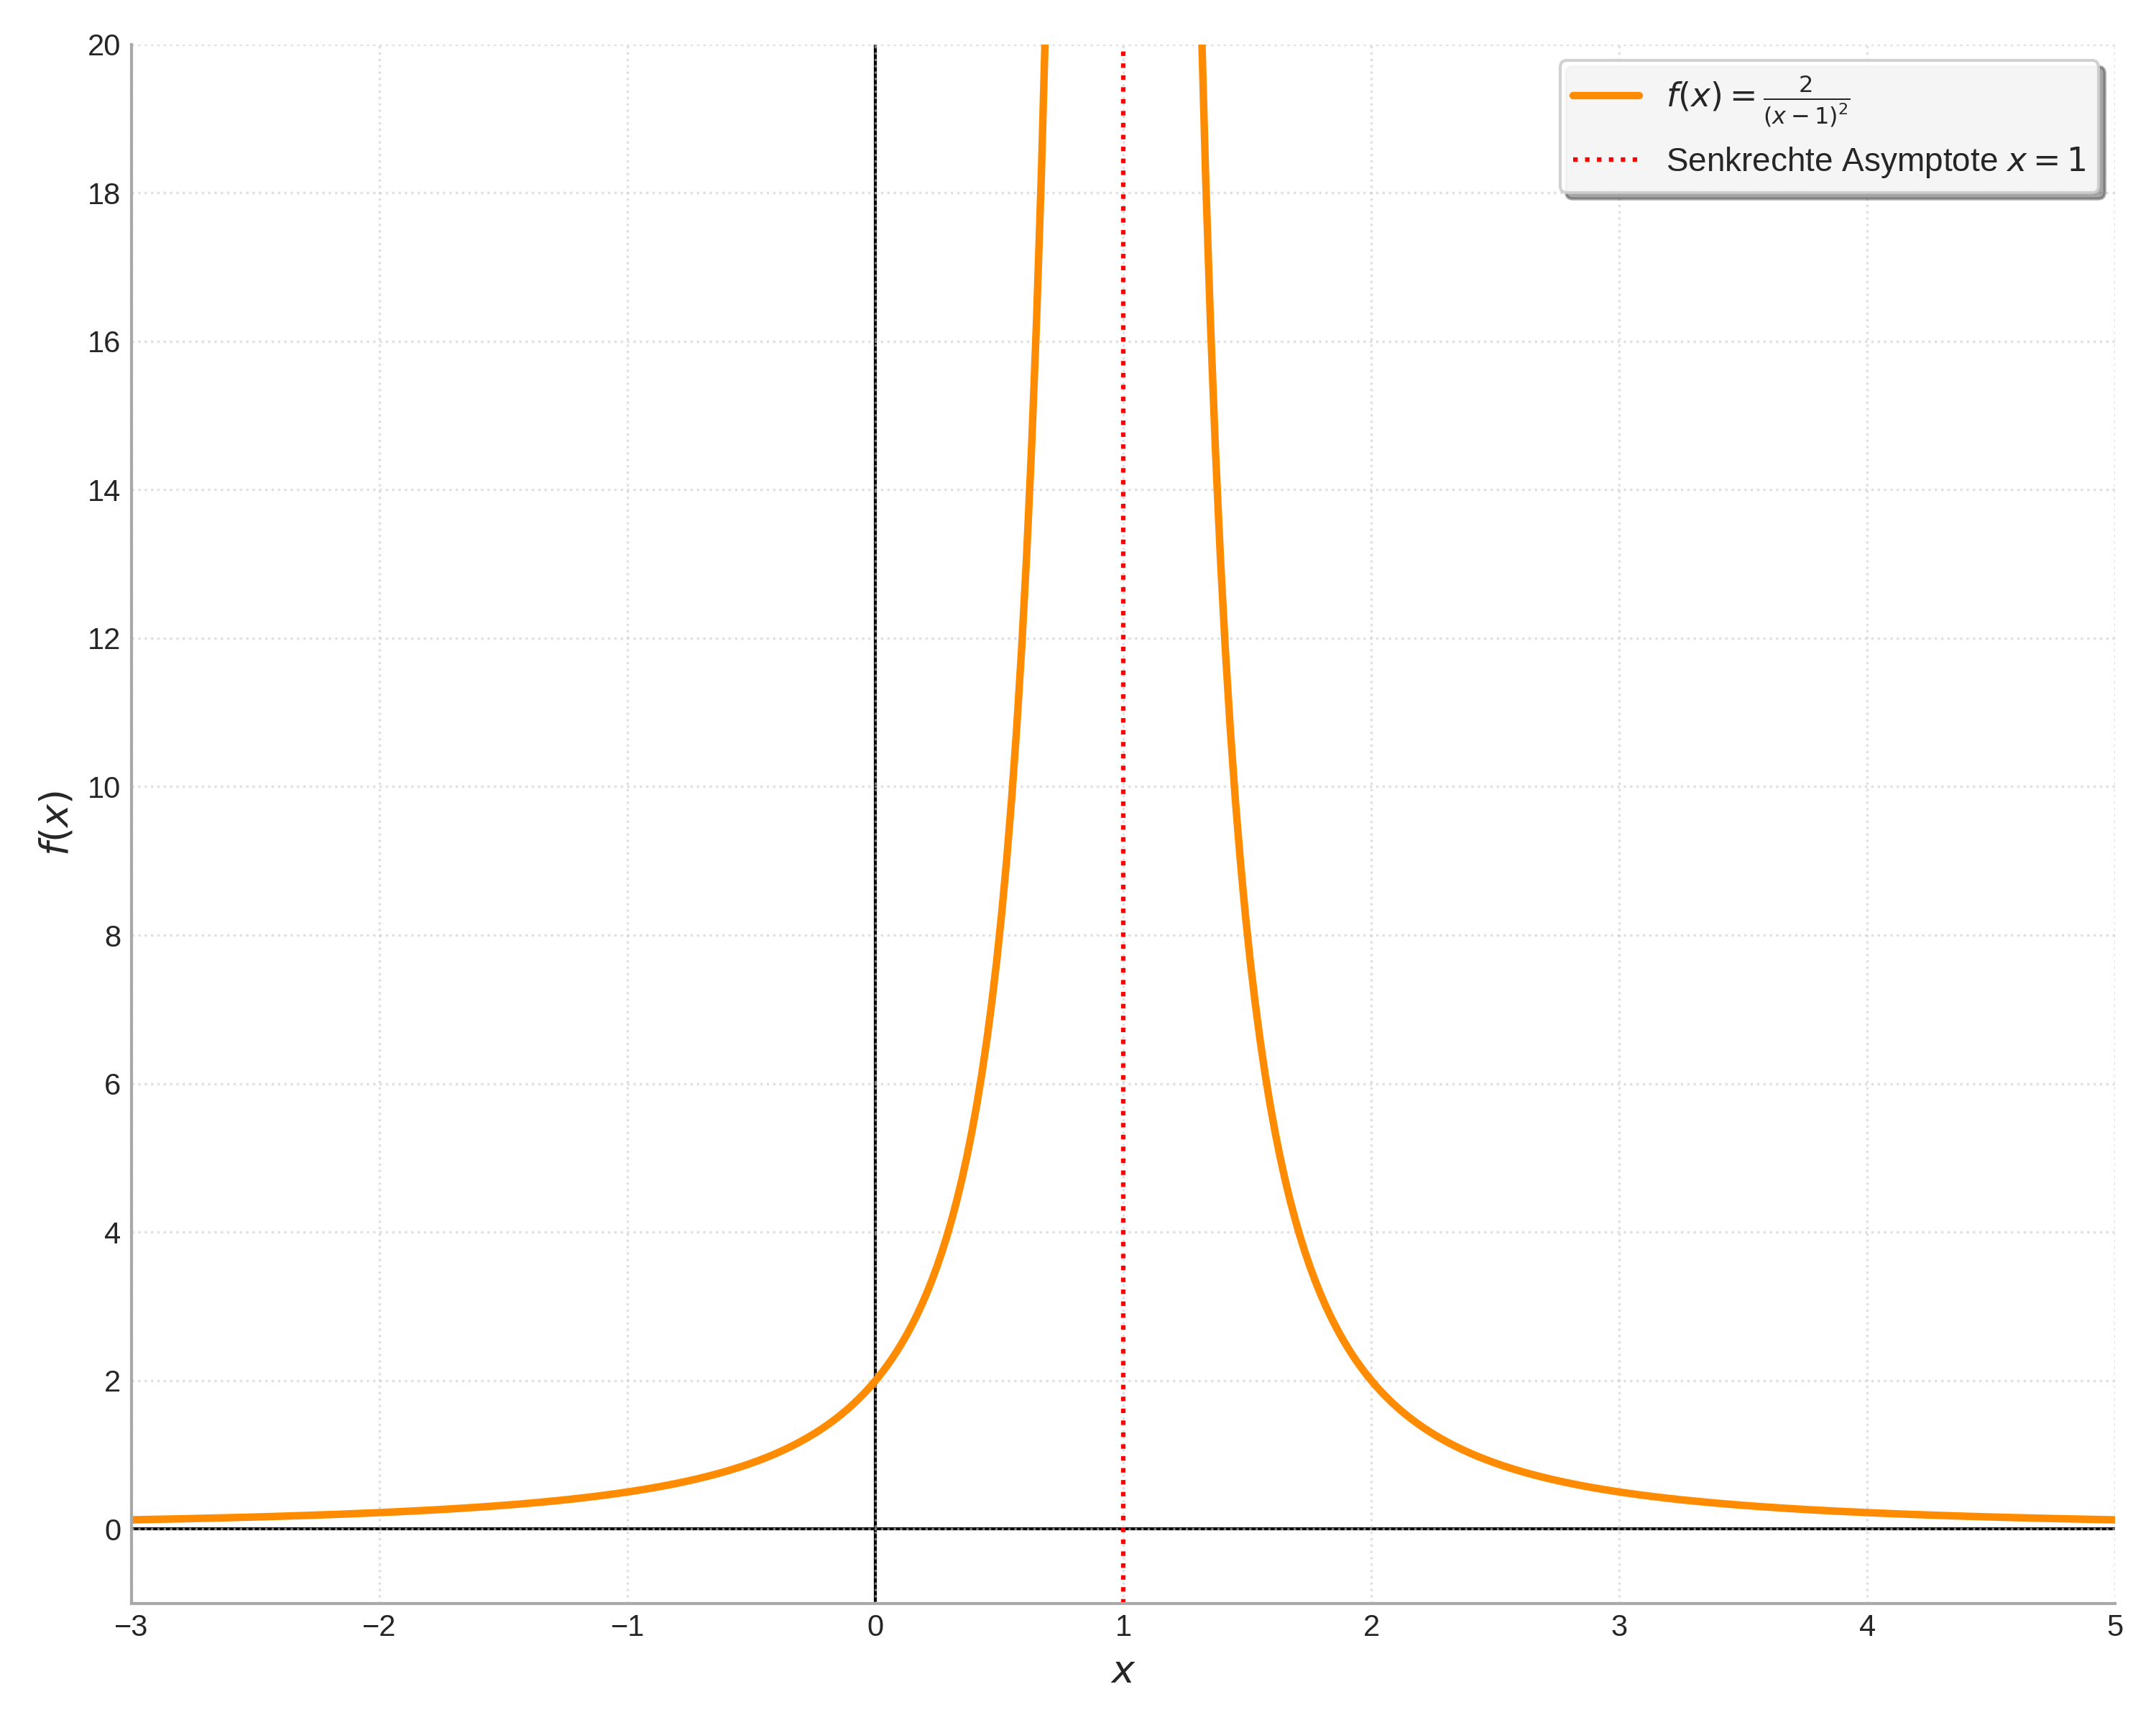
\includegraphics[width=0.8\textwidth]{grafiken/Gebrochen_Rational_Verschoben.png}
    \captionof{figure}{Graph von $f(x)=\frac{2}{(x-1)^2}$}
    \label{fig:gebr_rat_verschoben}
\end{center}
\end{beispielumgebung}

\begin{aufgabenumgebung}{Funktionen mit negativen Exponenten und Substitution}
\begin{enumerate}
    \item Bestimme für die folgenden Funktionen den Definitionsbereich, die Gleichung der senkrechten Asymptote(n) und das Verhalten der Funktion für $x$ gegen die Polstelle(n) (einseitige Grenzwerte) sowie für $x \to \pm\infty$. Untersuche auch das Symmetrieverhalten bezüglich der senkrechten Asymptote oder eines Punktes.
        \begin{itemize}
            \item $f_1(x) = \frac{-1}{x+2}$
            \item $f_2(x) = \frac{3}{(x-3)^2}$
            \item $f_3(x) = 1 - \frac{1}{x^2}$ (Tipp: Was ist hier die horizontale Asymptote?)
        \end{itemize}
    \item Skizziere die Graphen der Funktionen aus Teilaufgabe 1.
    \item \textbf{Transformationskette verstehen:}
        Beschreibe, wie der Graph der Funktion $g(x) = \frac{-2}{(x+3)^2} - 4$ aus dem Graphen der Grundfunktion $h(u) = \frac{1}{u^2}$ durch Streckung/Stauchung, Spiegelung und Verschiebungen hervorgeht. Gib den Definitionsbereich und die Gleichungen der Asymptoten von $g(x)$ an.
\end{enumerate}
\end{aufgabenumgebung}

\begin{kurzknappumgebung}{Funktionen $f(x) = \frac{a}{(x-c)^n} + d$}
\begin{itemize}
    \item \textbf{Definitionsbereich:} $D_f = \mathbb{R} \setminus \{c\}$.
    \item \textbf{Senkrechte Asymptote (Polstelle):} Bei $x=c$. Verhalten wie bei $\frac{a}{u^n}$ für $u \to 0$.
    \item \textbf{Waagerechte Asymptote:} Bei $y=d$. $\lim_{x \to \pm\infty} f(x) = d$. (Wenn $d=0$, ist es die x-Achse).
    \item \textbf{Symmetrie:} Wenn die Grundfunktion $\frac{a}{u^n}$ symmetrisch zum Ursprung (n ungerade) oder zur y-Achse (n gerade) ist, dann ist $f(x)$ symmetrisch zum Punkt $(c|d)$ bzw. zur Achse $x=c$.
\end{itemize}
\end{kurzknappumgebung}

\begin{fehlerboxumgebung}{Grenzwerte und Asymptoten}
\begin{itemize}
    \item \textbf{Verschiebung nicht erkannt:} Bei Termen wie $\frac{1}{x-c}$ liegt die Polstelle bei $x=c$, nicht bei $x=0$.
    \item \textbf{Horizontale Asymptote bei Summen/Differenzen:} Bei $f(x) = \frac{a}{x^n} + d$ ist die horizontale Asymptote $y=d$, nicht $y=0$ (außer $d=0$). Der Term $\frac{a}{x^n}$ geht gegen Null, aber das $d$ bleibt!
    \item \textbf{Definitionsbereich und Polstellen:} Eine Polstelle ist immer außerhalb des Definitionsbereichs.
\end{itemize}
\end{fehlerboxumgebung}

Wir werden diese Ideen zu Grenzwerten und Asymptoten später bei der Diskussion komplexerer gebrochen-rationaler Funktionen wieder aufgreifen. Jetzt, da wir ein solides Fundament für Polynome und einfache gebrochen-rationale Funktionen gelegt haben, können wir unseren Werkzeugkasten der Ableitungsregeln erweitern.
\subsection{Anwendung und Vertiefung der bisherigen Differentialrechnung}
\label{subsec:anwendung_vertiefung_diff_neu}

Wir haben nun die Grundlagen der Differentialrechnung kennengelernt: die Idee der Ableitung als momentane Änderungsrate und Tangentensteigung, die h-Methode zur Herleitung von Ableitungen sowie die ersten wichtigen Ableitungsregeln (Konstanten-, Potenz-, Faktor- und Summenregel). Wir haben auch gesehen, wie uns die erste und zweite Ableitung helfen, das Verhalten von Funktionen (Monotonie, Extrempunkte, Krümmung, Wendepunkte) zu analysieren und wie Grenzwerte das Verhalten im Unendlichen und an Polstellen beschreiben.

Bevor wir uns weiteren, komplexeren Ableitungsregeln zuwenden, wollen wir dieses Wissen festigen und in anspruchsvolleren Aufgaben anwenden.

\begin{kurzknappumgebung}{Differentialrechnung – Die Grundlagen im Überblick}
\begin{itemize}
    \item \textbf{Ableitung $f'(x)$:} Momentane Änderungsrate von $f(x)$; Steigung der Tangente an den Graphen von $f(x)$.
    \item \textbf{h-Methode:} Grundlegendes Verfahren zur Bestimmung der Ableitung über den Grenzwert des Differenzenquotienten: $f'(x_0) = \lim_{h \to 0} \frac{f(x_0+h) - f(x_0)}{h}$.
    \item \textbf{Wichtige Ableitungsregeln (bisher):}
        \begin{itemize}
            \item Konstantenregel: $(c)' = 0$.
            \item Potenzregel: $(x^n)' = nx^{n-1}$. (Gilt auch für negative/gebrochene Exponenten!)
            \item Faktorregel: $(c \cdot g(x))' = c \cdot g'(x)$.
            \item Summenregel: $(g(x) \pm h(x))' = g'(x) \pm h'(x)$.
        \end{itemize}
    \item \textbf{Bedeutung von $f'(x)$:}
        \begin{itemize}
            \item $f'(x) > 0 \implies f(x)$ ist streng monoton steigend.
            \item $f'(x) < 0 \implies f(x)$ ist streng monoton fallend.
            \item $f'(x_E) = 0$: Notwendige Bedingung für eine Extremstelle bei $x_E$.
            \item VZW von $f'$ an $x_E$: Hinreichende Bedingung für Extremstellen (Hoch-/Tiefpunkt).
        \end{itemize}
    \item \textbf{Bedeutung von $f''(x)$ (zweite Ableitung):}
        \begin{itemize}
            \item $f''(x) > 0 \implies$ Graph von $f(x)$ ist linksgekrümmt (konvex).
            \item $f''(x) < 0 \implies$ Graph von $f(x)$ ist rechtsgekrümmt (konkav).
            \item $f''(x_W) = 0$: Notwendige Bedingung für eine Wendestelle bei $x_W$.
            \item VZW von $f''$ an $x_W$ (oder $f'''(x_W) \neq 0$): Hinreichende Bedingung für Wendestelle.
            \item $f'(x_E)=0$ und $f''(x_E) > 0 \implies$ Tiefpunkt; $f'(x_E)=0$ und $f''(x_E) < 0 \implies$ Hochpunkt.
        \end{itemize}
    \item \textbf{Grenzwerte ($\lim$):} Untersuchen das Verhalten von Funktionen für $x \to \pm\infty$ oder an Definitionslücken (z.B. Polstellen bei $f(x)=a/x^n$).
    \item \textbf{Kurvendiskussion:} Systematische Untersuchung einer Funktion auf ihre Eigenschaften (Definitionsbereich, Symmetrie, Grenzwerte, Achsenschnittpunkte, Extrempunkte, Wendepunkte, Monotonie, Krümmung) zur Erstellung einer Graphenskizze.
    \item \textbf{Substitution als Denkwerkzeug:} Erkennen von Grundfunktionen in transformierter Form (z.B. $g(x) = \frac{a}{(x-c)^n}+d$ als Transformation von $f(u)=\frac{a}{u^n}$).
\end{itemize}
\end{kurzknappumgebung}

\begin{warumwichtigumgebung}{Was du jetzt können solltest}
Nachdem du diesen ersten Teil des Kapitels Differentialrechnung durchgearbeitet hast, solltest du in der Lage sein:
\begin{itemize}
    \item Den Begriff der Ableitung als momentane Änderungsrate und Tangentensteigung zu erklären.
    \item Die grundlegenden Ableitungsregeln (Konstanten-, Potenz-, Faktor-, Summenregel) sicher anzuwenden, auch auf Terme mit Wurzeln oder $x$ im Nenner (nach Umformung in Potenzschreibweise).
    \item Höhere Ableitungen zu bilden.
    \item Die Bedeutung der ersten und zweiten Ableitung für Monotonie, Extrempunkte, Krümmungsverhalten und Wendepunkte zu verstehen und anzuwenden.
    \item Das Grenzwertverhalten von Polynomfunktionen und einfachen gebrochen-rationalen Funktionen (wie $a/x^n$ und deren Verschiebungen) für $x \to \pm\infty$ und an Polstellen zu bestimmen.
    \item Eine vollständige Kurvendiskussion für Polynomfunktionen bis zum Grad 4 (mit lösbaren Nullstellenproblemen) und für einfache transformierte gebrochen-rationale Funktionen durchzuführen.
    \item Die Idee der Substitution zu nutzen, um das Verhalten transformierter Funktionen zu verstehen.
    \item Einfache Anwendungsaufgaben zu lösen, bei denen Änderungsraten oder Optimierungsprobleme eine Rolle spielen.
\end{itemize}
Das ist schon eine ganze Menge! Sei stolz auf das, was du gelernt hast. Die folgenden Aufgaben helfen dir, dein Wissen zu festigen und zu vertiefen.
\end{warumwichtigumgebung}

\begin{aufgabenumgebung}[A:DiffUebergreifend]{Übergreifende Übungsaufgaben zum bisherigen Kapitel Differentialrechnung}
\begin{enumerate}
    \item \textbf{Polynom-Analyse (Grad 3):}
        Gegeben ist die Funktion $f(x) = -\frac{1}{3}x^3 + x^2 + 3x - \frac{7}{3}$.
        \begin{enumerate}
            \item Führe eine vollständige Kurvendiskussion für $f(x)$ durch (Definitionsbereich, Symmetrie, Verhalten im Unendlichen, Achsenschnittpunkte, Extrempunkte, Wendepunkte, Monotonie, Krümmung).
            \begin{tippumgebung}{Nullstellen}
            Eine Nullstelle dieser Funktion ist $x_1=1$. Nutze diese Information, um die weiteren Nullstellen zu finden (z.B. durch Faktorisieren, nachdem du $(x-1)$ als Faktor erkannt hast, oder indem du die verbleibende quadratische Gleichung löst).
            \end{tippumgebung}
            \item Zeichne den Graphen von $f(x)$ im Intervall $[-4, 6]$ unter Verwendung deiner Ergebnisse.
            \item Bestimme die Gleichung der Tangente an den Graphen von $f(x)$ im Punkt $P(0|f(0))$.
            \item In welchem Punkt hat die Tangente an den Graphen von $f(x)$ die Steigung $m=-5$?
        \end{enumerate}
    \item \textbf{Optimierungsproblem – Die optimale Dose:}
        Eine zylinderförmige Konservendose soll ein Volumen von $V = 500 \text{ cm}^3$ haben. Die Materialkosten sollen minimiert werden, d.h. die Oberfläche $O$ der Dose soll minimal werden.
        Die Formeln für einen Zylinder mit Radius $r$ und Höhe $h$ sind:
        Volumen: $V = \pi r^2 h$
        Oberfläche (Mantel + 2 Deckel): $O = 2\pi r^2 + 2\pi r h$
        \begin{enumerate}
            \item \textbf{Zielfunktion aufstellen:} Drücke die Oberfläche $O$ als Funktion nur einer Variablen (z.B. des Radius $r$) aus. Nutze dazu die Nebenbedingung für das Volumen $V=500 \text{ cm}^3$, um $h$ durch $r$ auszudrücken und in die Oberflächenformel einzusetzen. Du erhältst $O(r)$.
            \begin{tippumgebung}{Umgang mit $\pi$}
            Behandle $\pi$ wie eine Konstante.
            \end{tippumgebung}
            \item \textbf{Ableitung bilden:} Bilde die erste Ableitung $O'(r)$. (Hinweis: $O(r)$ wird einen Term der Form $\frac{k}{r}$ enthalten, was du als $kr^{-1}$ schreiben kannst.)
            \item \textbf{Extremstelle finden:} Setze $O'(r)=0$ und löse nach $r$ auf, um den Radius zu finden, der die Oberfläche minimiert.
            \item \textbf{Überprüfung (optional für Experten):} Überprüfe mit der zweiten Ableitung $O''(r)$, ob es sich tatsächlich um ein Minimum handelt.
            \item \textbf{Optimale Abmessungen:} Berechne die zugehörige Höhe $h$ und das minimale Oberflächenmaterial. Welcher Zusammenhang besteht zwischen $r$ und $h$ bei minimaler Oberfläche?
        \end{enumerate}
    \item \textbf{Analyse einer biquadratischen Funktion:}
        Gegeben ist die Funktion $f(x) = x^4 - 8x^2 + 7$.
        \begin{enumerate}
            \item Untersuche die Funktion auf Symmetrie.
            \item Bestimme die Nullstellen der Funktion. (Tipp: Substitution $z=x^2$).
            \item Bestimme die lokalen Extrempunkte von $f(x)$.
            \item Bestimme die Wendepunkte von $f(x)$.
            \item Skizziere den Graphen von $f(x)$ basierend auf deinen Ergebnissen.
        \end{enumerate}
    \item \textbf{Transformationen und Grenzwerte verstehen:}
        Betrachte die Funktion $g(x) = \frac{-2}{(x+1)^3} + 1$.
        \begin{enumerate}
            \item \textbf{Grundfunktion:} Von welcher einfachen Grundfunktion $h(u) = \frac{a}{u^n}$ lässt sich $g(x)$ ableiten?
            \item \textbf{Transformationsschritte:} Beschreibe, durch welche Verschiebungen, Streckungen oder Spiegelungen der Graph von $g(x)$ aus dem Graphen von $h(u)$ entsteht.
            \item \textbf{Definitionsbereich und Asymptoten:} Bestimme den Definitionsbereich von $g(x)$ sowie die Gleichungen der senkrechten und waagerechten Asymptoten.
            \item \textbf{Grenzwerte an der Polstelle:} Untersuche $\lim_{x \to -1^+} g(x)$ und $\lim_{x \to -1^-} g(x)$. Handelt es sich um eine Polstelle mit oder ohne Vorzeichenwechsel?
            \item \textbf{Skizze:} Skizziere den Graphen von $g(x)$ mit seinen Asymptoten.
        \end{enumerate}
    \item \textbf{Bewegung eines Objekts (Anwendung):}
        Die Höhe $h$ (in Metern) eines senkrecht nach oben geworfenen Steins nach $t$ Sekunden wird durch die Funktion $h(t) = -5t^2 + 20t + 1$ beschrieben (für $t \ge 0$ und solange $h(t) \ge 0$).
        \begin{enumerate}
            \item Bestimme die Funktion $v(t)$, die die Geschwindigkeit des Autos zum Zeitpunkt $t$ angibt.
            \item Bestimme die Funktion $a(t)$, die die Beschleunigung des Autos zum Zeitpunkt $t$ angibt.
            \item Zu welchen Zeitpunkten $t$ ist das Auto in Ruhe (Geschwindigkeit gleich Null)?
            \item In welchen Zeitintervallen fährt das Auto vorwärts ($v(t)>0$) und in welchen rückwärts ($v(t)<0$)?
            \item Wann ist die Beschleunigung Null? Was bedeutet das für die Geschwindigkeit zu diesem Zeitpunkt?
            \item (Für Experten): Wann ist die Geschwindigkeit des Autos am größten im Intervall $[0, 2]$? Wann ist sie am geringsten (d.h. am stärksten negativ) im Intervall $[0, 4]$?
        \end{enumerate}
\end{enumerate}
\end{aufgabenumgebung}

\begin{infoboxumgebung}{Ein kleiner Exkurs: Was ist eigentlich Polynomdivision?}
Du hast in einigen Aufgaben den Hinweis auf 'Polynomdivision' gesehen, wenn es darum ging, Nullstellen von Polynomen höheren Grades (Grad > 2) zu finden, nachdem eine Nullstelle $x_1$ bereits bekannt war (z.B. durch Raten). Aber was steckt dahinter?

Stell dir vor, du hast ein Polynom $f(x)$ und kennst eine Nullstelle $x_1$. Das bedeutet, $(x-x_1)$ ist ein Faktor von $f(x)$ (genau wie wenn 12 durch 3 teilbar ist, weil 3 ein Faktor von 12 ist). Die Polynomdivision ist nun ein Verfahren, ähnlich der schriftlichen Division von Zahlen, mit dem du $f(x)$ durch den Linearfaktor $(x-x_1)$ teilen kannst.
\[ f(x) : (x-x_1) = \text{Restpolynom} \]
Das Ergebnis ist ein 'Restpolynom', dessen Grad um 1 niedriger ist als der von $f(x)$. Wenn $f(x)$ also z.B. vom Grad 3 war, ist das Restpolynom vom Grad 2. Und die Nullstellen eines quadratischen Polynoms können wir ja mit der p-q-Formel oder Mitternachtsformel finden!

\textbf{Beispiel-Idee:}
Wenn $f(x) = x^3 - 7x - 6$ und wir wissen (durch Raten), dass $x_1 = -1$ eine Nullstelle ist (denn $f(-1) = (-1)^3 - 7(-1) - 6 = -1 + 7 - 6 = 0$), dann können wir $f(x)$ durch $(x - (-1)) = (x+1)$ teilen.
\[
\polyset{style=C, vars=x, div=:} % Setzt den Divisionsoperator auf ':'
\polylongdiv{x^3 - 7x - 6}{x+1}
\]
(Die $0x^2$ wird für das schriftliche Verfahren oft ergänzt.)
Das Restpolynom $x^2 - x - 6$ können wir nun mit der p-q-Formel lösen, um die weiteren Nullstellen $x_2=3$ und $x_3=-2$ zu finden.

Die Polynomdivision ist also ein nützliches Werkzeug, um Polynome höheren Grades in Faktoren zu zerlegen und so alle Nullstellen zu finden. Das genaue Verfahren der schriftlichen Polynomdivision findest du in vielen Schulbüchern oder Online-Quellen, falls es dich genauer interessiert!
\end{infoboxumgebung}

\begin{infoboxumgebung}{Noch ein faszinierender Grenzwert: Die Eulersche Zahl $e$}
Wir haben den Grenzwertbegriff im Zusammenhang mit der Ableitung ($h \to 0$) und dem Verhalten von Funktionen im Unendlichen ($x \to \pm\infty$) kennengelernt. Es gibt noch viele andere wichtige Grenzwerte in der Mathematik. Einer davon führt zu einer ganz besonderen Zahl, der \textbf{Eulerschen Zahl $e \approx 2,71828\dots$}.

Stell dir vor, du legst 1 Euro zu 100\% Zinsen pro Jahr an.
\begin{itemize}
    \item Bei jährlicher Verzinsung hast du nach einem Jahr: $1 \cdot (1 + \frac{1}{1})^1 = 2$ Euro.
    \item Bei halbjährlicher Verzinsung (also $2 \times 50\%$ Zinsen): $1 \cdot (1 + \frac{1}{2})^2 = (1.5)^2 = 2,25$ Euro.
    \item Bei vierteljährlicher Verzinsung ($4 \times 25\%$ Zinsen): $1 \cdot (1 + \frac{1}{4})^4 \approx 2,44$ Euro.
    \item Bei monatlicher Verzinsung ($12 \times \frac{100}{12}\%$ Zinsen): $1 \cdot (1 + \frac{1}{12})^{12} \approx 2,61$ Euro.
\end{itemize}
Was passiert, wenn man die Zinsperioden immer kürzer macht und $n$-mal pro Jahr verzinst (also mit $\frac{100}{n}\%$ Zinsen pro Periode)? Man betrachtet den Ausdruck:
\[ \left(1 + \frac{1}{n}\right)^n \]
Wenn $n$ nun unendlich groß wird ($n \to \infty$), also die Verzinsung quasi kontinuierlich (in jedem unendlich kleinen Augenblick) erfolgt, dann nähert sich dieser Ausdruck einem festen Wert:
\[ \lim_{n \to \infty} \left(1 + \frac{1}{n}\right)^n = e \]
Die Zahl $e$ ist die Basis des \textbf{natürlichen Logarithmus} ($\ln$) und spielt eine fundamentale Rolle bei Exponentialfunktionen, die natürliches Wachstum oder Zerfall beschreiben (z.B. $f(x) = e^x$). Diese Funktionen werden wir in einem späteren Kapitel genauer untersuchen.
\end{infoboxumgebung}

\begin{infoboxumgebung}{Ausblick auf weitere Ableitungsregeln}
Mit den bisher gelernten Regeln (Konstanten-, Potenz-, Faktor-, Summenregel) können wir schon viele Funktionen, insbesondere alle Polynomfunktionen, ableiten und analysieren. Für komplexere Funktionen, die durch Multiplikation, Division oder Verkettung anderer Funktionen entstehen (wie z.B. $f(x) = x^2 \cdot e^x$, $g(x) = \frac{\sin(x)}{x}$ oder $h(x) = \sqrt{x^2+1}$), benötigen wir weitere Werkzeuge: die Produktregel, die Quotientenregel und die Kettenregel. Diese werden wir im nächsten Abschnitt kennenlernen.
\end{infoboxumgebung}

\subsection{Ableitungsregeln - Fortsetzung}

\subsubsection{Die Produktregel – Ableiten von $f(x) = u(x) \cdot v(x)$}
\label{subsubsec:produktregel}

Bisher haben wir Funktionen betrachtet, die Summen, Differenzen oder Vielfache von Potenzfunktionen waren. Was aber, wenn eine Funktion selbst ein Produkt aus zwei Funktionen ist, die beide die Variable $x$ enthalten? 
Ein Beispiel hierfür wäre $f(x) = (x^2+1)(x^3-2x)$.

Man könnte nun denken, man leitet einfach jeden Faktor einzeln ab und multipliziert die Ergebnisse. \textbf{Aber Vorsicht, das ist im Allgemeinen falsch!}
Also: $(u(x) \cdot v(x))' \neq u'(x) \cdot v'(x)$.

Um solche Produkte korrekt ableiten zu können, benötigen wir die \textbf{Produktregel}.

\begin{merksatzumgebung}{Produktregel}
Ist eine Funktion $f(x)$ als Produkt zweier differenzierbarer Funktionen $u(x)$ und $v(x)$ gegeben, also $f(x) = u(x) \cdot v(x)$, dann lautet ihre Ableitung:
\[ f'(x) = u'(x) \cdot v(x) + u(x) \cdot v'(x) \]
In Kurzschreibweise: $(u \cdot v)' = u'v + uv'$.
\end{merksatzumgebung}

\begin{tippumgebung}{Merkspruch für die Produktregel}
Ein gängiger Merkspruch, um sich die Produktregel einzuprägen, lautet:
'Ableitung des ersten Faktors mal den zweiten Faktor (stehen lassen), plus den ersten Faktor (stehen lassen) mal die Ableitung des zweiten Faktors.'
Oder noch kürzer: 'Erste ableiten, Zweite stehen lassen, plus Erste stehen lassen, Zweite ableiten.'
\end{tippumgebung}

Schauen wir uns an, wie das funktioniert und warum es so wichtig ist, diese Regel zu verwenden.

\begin{beispielumgebung}{Anwendung der Produktregel bei Polynomen}
Wir wollen die Funktion $f(x) = (x^2+3x) \cdot (2x-1)$ ableiten.

\textbf{Methode 1: Mit der Produktregel}

\textbf{Schritt 1: Identifiziere $u(x)$ und $v(x)$.}
$u(x) = x^2+3x$
$v(x) = 2x-1$

\textbf{Schritt 2: Bilde die Ableitungen $u'(x)$ und $v'(x)$.}
Mit den uns bekannten Regeln (Potenz-, Faktor-, Summenregel):
$u'(x) = (x^2)' + (3x)' = 2x + 3$
$v'(x) = (2x)' - (1)' = 2 - 0 = 2$

\textbf{Schritt 3: Setze in die Produktregel $f'(x) = u'(x)v(x) + u(x)v'(x)$ ein.}
$f'(x) = (2x+3) \cdot (2x-1) + (x^2+3x) \cdot (2)$

\textbf{Schritt 4: Vereinfache den Term (ausmultiplizieren und zusammenfassen).}
$f'(x) = (2x \cdot 2x + 2x \cdot (-1) + 3 \cdot 2x + 3 \cdot (-1)) + (2 \cdot x^2 + 2 \cdot 3x)$
$f'(x) = (4x^2 - 2x + 6x - 3) + (2x^2 + 6x)$
$f'(x) = 4x^2 + 4x - 3 + 2x^2 + 6x$
$f'(x) = (4x^2 + 2x^2) + (4x + 6x) - 3$
\[ f'(x) = 6x^2 + 10x - 3 \]

\textbf{Methode 2: Probe durch vorheriges Ausmultiplizieren (ohne Produktregel)}
Wir können die Funktion $f(x)$ auch zuerst ausmultiplizieren und dann die Summen- und Potenzregel anwenden:
$f(x) = (x^2+3x)(2x-1)$
$f(x) = x^2 \cdot 2x + x^2 \cdot (-1) + 3x \cdot 2x + 3x \cdot (-1)$
$f(x) = 2x^3 - x^2 + 6x^2 - 3x$
$f(x) = 2x^3 + ( -x^2 + 6x^2) - 3x$
$f(x) = 2x^3 + 5x^2 - 3x$

Nun leiten wir diese Summe ab:
$f'(x) = (2x^3)' + (5x^2)' - (3x)'$
$f'(x) = 2 \cdot 3x^2 + 5 \cdot 2x - 3 \cdot 1$
\[ f'(x) = 6x^2 + 10x - 3 \]
Beide Methoden führen zum selben Ergebnis! Das zeigt, dass die Produktregel korrekt ist und uns bei komplizierteren Produkten, die sich nicht so leicht ausmultiplizieren lassen (z.B. wenn $e$-Funktionen oder trigonometrische Funktionen beteiligt sind), eine große Hilfe sein wird.
\end{beispielumgebung}

\textit{Selbst-Check:} Warum ist es bei $f(x) = 5x^3$ nicht notwendig, die Produktregel anzuwenden, obwohl man es als $u(x)=5$ und $v(x)=x^3$ auffassen könnte? (Antwort: Weil $u(x)=5$ eine Konstante ist. Die Faktorregel ist ein Spezialfall der Produktregel, wenn einer der Faktoren eine Konstante ist: $(c \cdot v(x))' = c' \cdot v(x) + c \cdot v'(x) = 0 \cdot v(x) + c \cdot v'(x) = c \cdot v'(x)$.)

\begin{aufgabenumgebung}{Produktregel trainieren}
Leite die folgenden Funktionen mit der Produktregel ab und vereinfache die Ergebnisse so weit wie möglich. Kontrolliere deine Ergebnisse für die ersten beiden Aufgaben, indem du die Terme zuerst ausmultiplizierst und dann ableitest.
\begin{enumerate}
    \item $f(x) = (x+2)(3x-4)$
    \item $g(x) = x^2(x^3+5x)$
    \item $h(t) = (t^2-1)(t^2+1)$ (Erkennst du hier eine binomische Formel, die das Ausmultiplizieren erleichtert?)
    \item $k(x) = (2x^3-x)(x^2+x+1)$
    \item $m(a) = (a^2+1)(a-1)$ (Leite nach $a$ ab.)
\end{enumerate}
\end{aufgabenumgebung}

\begin{warumwichtigumgebung}{Die Produktregel}
Die Produktregel ist unerlässlich, sobald Funktionen multiplikativ verknüpft sind und beide Faktoren von der Variablen abhängen. Viele reale Modelle entstehen durch Produkte von Funktionen (z.B. Umsatz = Preis $\times$ Menge, wobei Preis und Menge von einer anderen Größe abhängen können). Ohne die Produktregel könnten wir solche Modelle nicht korrekt analysieren. Sie ist ein Grundpfeiler der Differentialrechnung.
\end{warumwichtigumgebung}

% Vorheriger Inhalt des Kapitels bis zur warumwichtigumgebung 'Die Produktregel'
% ... (siehe vorherige Canvas-Version) ...

% Vorheriger Inhalt des Kapitels bis zur warumwichtigumgebung 'Die Produktregel'
% ... (siehe vorherige Canvas-Version) ...

\begin{aufgabenumgebung}[A:ProduktregelAnwendung]{Anwendung der Produktregel in einer Kurvendiskussion (vereinfacht)}
Gegeben sei die Funktion $f(x) = x \cdot (x-3)^2$.
\begin{enumerate}
    \item \textbf{Definitionsbereich und Verhalten im Unendlichen:} Bestimme $D_f$ und untersuche $\lim_{x \to \pm\infty} f(x)$.
    \item \textbf{Nullstellen:} Bestimme die Nullstellen von $f(x)$ direkt aus der faktorisierten Form. Welche Vielfachheit haben sie? Was bedeutet das für den Graphen?
    \item \textbf{Erste Ableitung mit Produktregel:}
        Identifiziere $u(x)=x$ und $v(x)=(x-3)^2$. 
        \begin{tippumgebung}{Ableitung von $v(x)=(x-3)^2$}
        Um $v(x)=(x-3)^2$ abzuleiten, kannst du es entweder ausmultiplizieren zu $x^2-6x+9$ und dann die Summen-/Potenzregel anwenden, oder du erkennst hier schon eine verkettete Funktion (die Kettenregel lernen wir später noch genauer kennen). Für jetzt: $(x-c)^2$ abgeleitet ist $2(x-c)\cdot 1 = 2(x-c)$. Also ist $v'(x) = 2(x-3)$.
        \end{tippumgebung}
        Bilde $f'(x)$ mit der Produktregel. Vereinfache $f'(x)$ so weit wie möglich (Tipp: $(x-3)$ ausklammern).
    \item \textbf{Extremstellen:} Bestimme die Nullstellen von $f'(x)$. Untersuche das Vorzeichen von $f'(x)$ (Monotonieintervalle), um die Art der Extremstellen zu bestimmen. Berechne die y-Koordinaten der Extrempunkte.
    \item \textbf{Skizze:} Skizziere den Graphen von $f(x)$ unter Verwendung deiner Ergebnisse.
\end{enumerate}
Diese Aufgabe zeigt, wie die Produktregel auch bei der Analyse von Polynomfunktionen nützlich sein kann, besonders wenn sie in faktorisierter Form vorliegen oder entstehen.
\end{aufgabenumgebung}

\subsubsection{Die Quotientenregel – Ableiten von $f(x) = \frac{u(x)}{v(x)}$}
\label{subsubsec:quotientenregel}

Nachdem wir Produkte ableiten können, stellt sich natürlich die Frage: Wie leitet man einen Bruch (Quotienten) von zwei Funktionen ab, bei dem die Variable $x$ sowohl im Zähler als auch im Nenner vorkommt? Ein Beispiel wäre $f(x) = \frac{x^2+1}{x-2}$.

Auch hier gilt: Man darf \textbf{nicht} einfach den Zähler und den Nenner getrennt ableiten und die Ergebnisse dividieren!
Also: $\left(\frac{u(x)}{v(x)}\right)' \neq \frac{u'(x)}{v'(x)}$.

Für Quotienten benötigen wir die \textbf{Quotientenregel}.

\begin{merksatzumgebung}{Quotientenregel}
Ist eine Funktion $f(x)$ als Quotient zweier differenzierbarer Funktionen $u(x)$ (Zähler) und $v(x)$ (Nenner) gegeben, also $f(x) = \frac{u(x)}{v(x)}$ (wobei $v(x) \neq 0$), dann lautet ihre Ableitung:
\[ f'(x) = \frac{u'(x) \cdot v(x) - u(x) \cdot v'(x)}{[v(x)]^2} \]
In Kurzschreibweise: $\left(\frac{u}{v}\right)' = \frac{u'v - uv'}{v^2}$.
\end{merksatzumgebung}

\textbf{Herleitung der Quotientenregel (für Interessierte):}
Wir können die Quotientenregel tatsächlich aus der Produktregel und der (später noch genauer behandelten) Kettenregel herleiten. Eine einfachere Herleitung für Polynome und Potenzfunktionen gelingt, wenn wir den Quotienten als Produkt umschreiben:
$f(x) = \frac{u(x)}{v(x)} = u(x) \cdot (v(x))^{-1}$.
Jetzt wenden wir die Produktregel $(fg)' = f'g + fg'$ an, wobei $g(x) = (v(x))^{-1}$.
Die Ableitung von $g(x)=(v(x))^{-1}$ ist nach der (verallgemeinerten) Potenzregel und Kettenregel $g'(x) = -1 \cdot (v(x))^{-2} \cdot v'(x) = -\frac{v'(x)}{(v(x))^2}$.
(Die Kettenregel besagt grob: äußere Ableitung mal innere Ableitung. Die äußere Funktion ist hier $(\dots)^{-1}$, ihre Ableitung ist $-1(\dots)^{-2}$. Die innere Funktion ist $v(x)$, ihre Ableitung ist $v'(x)$.)

Setzen wir dies in die Produktregel ein:
$f'(x) = u'(x) \cdot (v(x))^{-1} + u(x) \cdot \left( -1 \cdot (v(x))^{-2} \cdot v'(x) \right)$
$f'(x) = \frac{u'(x)}{v(x)} - \frac{u(x) \cdot v'(x)}{(v(x))^2}$
Um dies auf einen gemeinsamen Nenner zu bringen, erweitern wir den ersten Bruch mit $v(x)$:
$f'(x) = \frac{u'(x) \cdot v(x)}{v(x) \cdot v(x)} - \frac{u(x) \cdot v'(x)}{(v(x))^2}$
$f'(x) = \frac{u'(x) \cdot v(x) - u(x) \cdot v'(x)}{[v(x)]^2}$
Und das ist genau die Quotientenregel! Es ist schön zu sehen, wie die Regeln in der Mathematik zusammenhängen.

\begin{tippumgebung}{Merkspruch für die Quotientenregel}
Ein gängiger Merkspruch, der die Reihenfolge der Terme im Zähler betont (da hier ein Minuszeichen steht, ist die Reihenfolge wichtig!), lautet:
'Ableitung des Zählers mal Nenner (stehen lassen) \textbf{minus} Zähler (stehen lassen) mal Ableitung des Nenners, das Ganze geteilt durch den Nenner zum Quadrat.'
Oft abgekürzt als: \textbf{NAZ - ZAN} durch Nenner-Quadrat (Nenner mal Ableitung Zähler minus Zähler mal Ableitung Nenner).
\textbf{Achtung:} Der Merkspruch ist 'NAZ - ZAN', aber die Formel ist $u'v - uv'$. $u$ ist der Zähler, $v$ der Nenner. Also: $u'v - uv'$.
Ein anderer, vielleicht besserer Merkspruch ist: \textbf{'Nenner mal Ableitung Zähler minus Zähler mal Ableitung Nenner, durch Nenner hoch zwei.'} (N·AZ - Z·AN / N²)
Oder: 'Ableitung oben mal unten minus oben mal Ableitung unten, durch unten ins Quadrat.'
\end{tippumgebung}

Die Quotientenregel sieht auf den ersten Blick etwas komplizierter aus, aber mit Übung wird sie dir vertraut.

\begin{beispielumgebung}{Anwendung der Quotientenregel}
Wir wollen die Funktion $f(x) = \frac{x^2+1}{x-2}$ ableiten. (Definitionsbereich: $D_f = \mathbb{R} \setminus \{2\}$)

\textbf{Schritt 1: Identifiziere $u(x)$ (Zähler) und $v(x)$ (Nenner).}
$u(x) = x^2+1$
$v(x) = x-2$

\textbf{Schritt 2: Bilde die Ableitungen $u'(x)$ und $v'(x)$.}
$u'(x) = (x^2+1)' = 2x$
$v'(x) = (x-2)' = 1$

\textbf{Schritt 3: Setze in die Quotientenregel $f'(x) = \frac{u'(x)v(x) - u(x)v'(x)}{[v(x)]^2}$ ein.}
$f'(x) = \frac{(2x) \cdot (x-2) - (x^2+1) \cdot (1)}{(x-2)^2}$

\textbf{Schritt 4: Vereinfache den Zähler.}
$f'(x) = \frac{2x^2 - 4x - (x^2+1)}{(x-2)^2}$
$f'(x) = \frac{2x^2 - 4x - x^2 - 1}{(x-2)^2}$
\[ f'(x) = \frac{x^2 - 4x - 1}{(x-2)^2} \]
Den Nenner $(x-2)^2$ lässt man oft in dieser Form stehen und multipliziert ihn nicht aus, da er für die Bestimmung von Nullstellen der Ableitung (wenn der Zähler Null ist) oder für das Verhalten an der Polstelle ($x=2$) in dieser Form nützlicher ist.
\end{beispielumgebung}

\begin{fehlerboxumgebung}{Häufige Fehler bei der Quotientenregel}
\begin{itemize}
    \item \textbf{Reihenfolge im Zähler vertauscht:} Das Minuszeichen macht die Reihenfolge $u'v - uv'$ entscheidend! Ein Vertauschen führt zum falschen Vorzeichen.
    \item \textbf{Nenner nicht quadriert:} Der Nenner der Ableitung ist immer $[v(x)]^2$.
    \item \textbf{Klammern vergessen:} Besonders wenn $u(x)$ oder $v(x)$ Summen oder Differenzen sind, müssen beim Einsetzen in die Formel Klammern gesetzt werden, z.B. $u(x)v'(x)$ ist $(x^2+1) \cdot (1)$ und nicht $x^2+1 \cdot 1$.
    \item \textbf{Fehler beim Vereinfachen des Zählers:} Achte auf Vorzeichen, wenn du Klammern auflöst.
\end{itemize}
\end{fehlerboxumgebung}

\begin{aufgabenumgebung}{Quotientenregel trainieren}
Leite die folgenden Funktionen mit der Quotientenregel ab und vereinfache die Zähler der Ergebnisse so weit wie möglich. Gib auch den Definitionsbereich der ursprünglichen Funktion an.
\begin{enumerate}
    \item $f(x) = \frac{x}{x+1}$
    \item $g(x) = \frac{3x-2}{x^2}$ (Tipp: Dies könnte man auch als $g(x) = (3x-2)x^{-2}$ mit der Produktregel oder nach Aufteilen des Bruchs $\frac{3x}{x^2} - \frac{2}{x^2} = \frac{3}{x} - \frac{2}{x^2}$ mit Potenz-/Faktorregeln ableiten. Vergleiche die Ergebnisse!)
    \item $h(t) = \frac{t^2+2t}{t-1}$
    \item $k(x) = \frac{5}{2x+3}$ (Hier ist $u(x)=5$, also $u'(x)=0$. Was bedeutet das für die Formel?)
\end{enumerate}
\end{aufgabenumgebung}

\begin{warumwichtigumgebung}{Die Quotientenregel}
Die Quotientenregel ist notwendig, um gebrochen-rationale Funktionen korrekt ableiten zu können. Diese Funktionen spielen eine wichtige Rolle bei der Modellierung von Phänomenen, bei denen Verhältnisse oder Raten auftreten, die sich ändern, oder bei denen es Asymptoten gibt (z.B. Konzentrationen, Durchschnittskosten, bestimmte physikalische Gesetze). Ohne die Quotientenregel wären Kurvendiskussionen solcher Funktionen nicht möglich.
\end{warumwichtigumgebung}

\begin{kurzknappumgebung}{Produkt- und Quotientenregel}
\begin{itemize}
    \item \textbf{Produktregel $(u \cdot v)' = u'v + uv'$}: Anwenden, wenn zwei von $x$ abhängige Terme multipliziert werden.
    \item \textbf{Quotientenregel $(\frac{u}{v})' = \frac{u'v - uv'}{v^2}$}: Anwenden, wenn zwei von $x$ abhängige Terme dividiert werden (Bruch). Achte auf die Reihenfolge im Zähler!
    \item \textbf{Alternative bei Polynomen/einfachen Brüchen:} Manchmal ist Ausmultiplizieren (Produkt) oder Aufteilen des Bruchs (Quotient) und anschließendes Ableiten mit Summen-/Potenzregel einfacher oder eine gute Kontrollmöglichkeit.
\end{itemize}
\end{kurzknappumgebung}

\begin{aufgabenumgebung}{Anwendung der neuen Regeln in Kontexten}
\begin{enumerate}
    \item \textbf{Umsatzfunktion:} Ein Unternehmen verkauft ein Produkt. Die Preis-Absatz-Funktion (Nachfragefunktion) sei $p(x) = 100 - 0.5x$, wobei $x$ die verkaufte Menge und $p(x)$ der Preis pro Stück ist. Der Umsatz $U(x)$ ist Preis mal Menge, also $U(x) = p(x) \cdot x = (100-0.5x)x$.
        \begin{itemize}
            \item Bestimme die Umsatzfunktion $U(x)$.
            \item Bilde die erste Ableitung $U'(x)$ (Grenzerlös). Du kannst dies tun, indem du $U(x)$ zuerst ausmultiplizierst oder indem du die Produktregel auf $p(x) \cdot x$ anwendest. Vergleiche beide Wege.
            \item Bei welcher Verkaufsmenge $x$ wird der Grenzerlös Null? Was könnte das für den Gesamtumsatz bedeuten?
        \end{itemize}
    \item \textbf{Durchschnittskosten:} Die Kostenfunktion eines Unternehmens sei $K(x) = 0.1x^3 - 2x^2 + 50x + 100$. Die Durchschnittskosten (Stückkosten) sind $k(x) = \frac{K(x)}{x}$.
        \begin{itemize}
            \item Schreibe die Funktion für die Durchschnittskosten $k(x)$ auf.
            \item Bilde die erste Ableitung $k'(x)$ mit der Quotientenregel.
            \item (Für Experten): Versuche, die Stelle zu finden, an der die Durchschnittskosten minimal sind (also $k'(x)=0$ setzen und nach $x$ auflösen – das kann hier schwierig werden, aber der Ansatz ist wichtig).
        \end{itemize}
\end{enumerate}
\end{aufgabenumgebung}

% Vorheriger Inhalt des Kapitels bis zur aufgabenumgebung 'Anwendung der neuen Regeln in Kontexten'
% ... (siehe vorherige Canvas-Version) ...

% HIER FOLGT DANN DIE KETTENREGEL
% Dieser Kommentar wird durch den folgenden Inhalt ersetzt:

\subsubsection{Die Kettenregel – Ableiten von verketteten Funktionen $f(x) = g(h(x))$}
\label{subsubsec:kettenregel}

Wir haben gelernt, wie man Summen, Produkte und Quotienten von Funktionen ableitet. Aber was ist, wenn Funktionen ineinander 'verschachtelt' oder 'verkettet' sind? Stell dir eine Funktion vor wie eine Maschine: Du gibst $x$ hinein, die 'innere' Maschine $h$ macht etwas damit ($h(x)$), und dieses Ergebnis wird dann in eine 'äußere' Maschine $g$ gesteckt, die $g(h(x))$ produziert. Ein Beispiel wäre $f(x) = (2x+5)^3$. Hier ist die innere Funktion $h(x)=2x+5$ und die äußere Funktion $g(u)=u^3$.

Solche \textbf{verketteten Funktionen} (auch zusammengesetzte Funktionen genannt) können wir nicht einfach mit den bisherigen Regeln ableiten. Wir brauchen ein neues, sehr mächtiges Werkzeug: die \textbf{Kettenregel}.

\begin{merksatzumgebung}{Kettenregel}
Ist eine Funktion $f(x)$ als Verkettung zweier differenzierbarer Funktionen $g(u)$ (äußere Funktion) und $u=h(x)$ (innere Funktion) gegeben, also $f(x) = g(h(x))$, dann lautet ihre Ableitung:
\[ f'(x) = g'(h(x)) \cdot h'(x) \]
\textbf{In Worten:} 'Die Ableitung der äußeren Funktion (wobei die innere Funktion als Argument eingesetzt bleibt) multipliziert mit der Ableitung der inneren Funktion.'
Oder kurz: \textbf{Äußere Ableitung mal innere Ableitung.}
\end{merksatzumgebung}

\begin{infoboxumgebung}{Die Kettenregel verstehen – Wie eine Zwiebel oder Matrjoschka-Puppen}
Stell dir eine verkettete Funktion wie eine Zwiebel oder eine russische Matrjoschka-Puppe vor. Um zum Kern zu gelangen, musst du Schicht für Schicht 'ableiten':
\begin{enumerate}
    \item \textbf{Äußerste Schicht (äußere Funktion $g$):} Leite sie ab, aber behalte das, was 'innen' ist ($h(x)$), einfach bei. Das ist $g'(h(x))$.
    \item \textbf{Nächste Schicht (innere Funktion $h$):} Leite sie ab. Das ist $h'(x)$.
    \item \textbf{Multipliziere die Ergebnisse:} $g'(h(x)) \cdot h'(x)$.
\end{enumerate}
Wenn es mehrere Verschachtelungen gibt, z.B. $f(x) = a(b(c(x)))$, dann gilt die Regel entsprechend erweitert: $f'(x) = a'(b(c(x))) \cdot b'(c(x)) \cdot c'(x)$. Man leitet von außen nach innen ab und multipliziert die einzelnen Ableitungen.
\end{infoboxumgebung}

Schauen wir uns das an einem Beispiel an, das wir auch ohne Kettenregel (mit viel Mühe) lösen könnten.

\begin{beispielumgebung}{Anwendung der Kettenregel bei einer potenzierten Klammer}
Wir wollen die Funktion $f(x) = (2x+5)^3$ ableiten.

\textbf{Schritt 1: Identifiziere die äußere und innere Funktion.}
\begin{itemize}
    \item Die \textbf{innere Funktion} ist das, was in der Klammer potenziert wird: $h(x) = 2x+5$.
    \item Die \textbf{äußere Funktion} ist das Potenzieren mit 3: Wenn wir $u = h(x)$ setzen, ist $g(u) = u^3$.
\end{itemize}
Also $f(x) = g(h(x))$ mit $g(u)=u^3$ und $h(x)=2x+5$.

\textbf{Schritt 2: Bilde die Ableitungen der inneren und äußeren Funktion.}
\begin{itemize}
    \item Ableitung der inneren Funktion: $h'(x) = (2x+5)' = 2$.
    \item Ableitung der äußeren Funktion (nach ihrer Variablen $u$): $g'(u) = (u^3)' = 3u^2$.
\end{itemize}

\textbf{Schritt 3: Setze in die Kettenregel $f'(x) = g'(h(x)) \cdot h'(x)$ ein.}
\begin{itemize}
    \item $g'(h(x))$ bedeutet: Nimm die äußere Ableitung $g'(u)=3u^2$ und setze für $u$ wieder die innere Funktion $h(x)=2x+5$ ein.
    Also: $g'(h(x)) = 3(2x+5)^2$.
    \item $h'(x)$ hatten wir schon: $h'(x) = 2$.
\end{itemize}
Zusammengesetzt:
$f'(x) = \underbrace{3(2x+5)^2}_{g'(h(x))} \cdot \underbrace{2}_{h'(x)}$
\[ f'(x) = 6(2x+5)^2 \]

\textbf{Probe durch Ausmultiplizieren (optional und hier aufwendig):}
$(2x+5)^3 = (2x+5)(2x+5)(2x+5) = (4x^2+20x+25)(2x+5)$
$= 8x^3 + 20x^2 + 40x^2 + 100x + 50x + 125$
$= 8x^3 + 60x^2 + 150x + 125$.
Ableiten mit Summen-/Potenzregel:
$f'(x) = (8x^3)' + (60x^2)' + (150x)' + (125)'$
$f'(x) = 24x^2 + 120x + 150$.

Ist das dasselbe wie $6(2x+5)^2$?
$6(2x+5)^2 = 6((2x)^2 + 2 \cdot 2x \cdot 5 + 5^2) = 6(4x^2 + 20x + 25)$
$= 24x^2 + 120x + 150$. Ja, es stimmt!
Die Kettenregel war hier deutlich schneller als das Ausmultiplizieren.
\end{beispielumgebung}

\begin{tippumgebung}{Spezialfall der Kettenregel: Lineare innere Funktion}
Wenn die innere Funktion linear ist, also $h(x) = mx+b$, dann ist $h'(x)=m$.
Die Kettenregel für $f(x) = g(mx+b)$ lautet dann:
$f'(x) = g'(mx+b) \cdot m$.
Beispiel: $f(x) = (4x-7)^5$. Äußere Funktion $g(u)=u^5 \implies g'(u)=5u^4$. Innere Funktion $h(x)=4x-7 \implies h'(x)=4$.
$f'(x) = 5(4x-7)^4 \cdot 4 = 20(4x-7)^4$.
\end{tippumgebung}

\begin{aufgabenumgebung}{Kettenregel trainieren}
Leite die folgenden Funktionen mit der Kettenregel ab. Identifiziere zuerst sorgfältig die äußere und die innere Funktion.
\begin{enumerate}
    \item $f(x) = (x^2+1)^4$
    \item $g(x) = (5-3x)^7$
    \item $h(t) = \sqrt{t^2+3t}$ (Tipp: $\sqrt{u} = u^{1/2}$)
    \item $k(x) = \frac{1}{(x^3-2x)^2}$ (Tipp: $k(x) = (x^3-2x)^{-2}$)
    \item $m(x) = (ax^2+b)^n$ (wobei $a,b,n$ Konstanten sind. Was ist die Ableitung?)
\end{enumerate}
\end{aufgabenumgebung}

\begin{fehlerboxumgebung}{Häufige Fehler bei der Kettenregel}
\begin{itemize}
    \item \textbf{Die innere Ableitung $h'(x)$ wird vergessen!} Das ist der häufigste Fehler. Man leitet die äußere Funktion ab und vergisst, mit der Ableitung der inneren Funktion zu multiplizieren.
    \item \textbf{Falsche Identifikation von äußerer und innerer Funktion:} Überlege dir genau, welche Operation 'zuerst' auf $x$ wirkt (innere Funktion) und welche 'danach' auf das Ergebnis (äußere Funktion).
    \item \textbf{Äußere Funktion nicht korrekt abgeleitet:} Wenn $g(u)=u^n$, dann ist $g'(u)=nu^{n-1}$. In $g'(h(x))$ muss dann für $u$ der gesamte innere Term $h(x)$ eingesetzt werden, bevor mit $h'(x)$ multipliziert wird.
\end{itemize}
\end{fehlerboxumgebung}

\begin{warumwichtigumgebung}{Die Kettenregel}
Die Kettenregel ist eine der wichtigsten und am häufigsten angewendeten Ableitungsregeln. Sehr viele Funktionen, denen wir begegnen, sind Verkettungen. Ohne die Kettenregel könnten wir Funktionen wie $e^{x^2}$, $\sin(3x)$, $\ln(x^2+1)$ oder $\sqrt{4-x^2}$ nicht ableiten. Sie ist der Schlüssel zur Analyse einer riesigen Klasse von Funktionen und deren Verhalten.
\end{warumwichtigumgebung}

\begin{kurzknappumgebung}{Kettenregel}
\begin{itemize}
    \item \textbf{Anwendung:} Für verkettete Funktionen $f(x) = g(h(x))$ ('Funktion in Funktion').
    \item \textbf{Formel:} $f'(x) = g'(h(x)) \cdot h'(x)$ ('Äußere Ableitung mal innere Ableitung').
    \item \textbf{Vorgehen:}
        \begin{enumerate}
            \item Innere Funktion $h(x)$ und äußere Funktion $g(u)$ identifizieren.
            \item Beide getrennt ableiten: $h'(x)$ und $g'(u)$.
            \item In $g'(u)$ für $u$ wieder $h(x)$ einsetzen, um $g'(h(x))$ zu erhalten.
            \item $g'(h(x))$ mit $h'(x)$ multiplizieren.
        \end{enumerate}
\end{itemize}
\end{kurzknappumgebung}


\subsubsection{Zusammenfassung und kombinierte Anwendung aller Ableitungsregeln}
\label{subsubsec:anwendung_aller_regeln_neu} % Neues Label

Jetzt, da wir die Konstanten-, Potenz-, Faktor-, Summen-, Produkt-, Quotienten- und Kettenregel kennen, haben wir einen mächtigen Werkzeugkasten, um eine sehr große Vielfalt von Funktionen zu differenzieren. Oft müssen wir mehrere dieser Regeln in einer einzigen Aufgabe geschickt kombinieren.

\begin{kurzknappumgebung}{Alle bisherigen Ableitungsregeln im Überblick}
\begin{itemize}
    \item \textbf{Konstantenregel:} $(c)' = 0$
    \item \textbf{Potenzregel:} $(x^n)' = nx^{n-1}$
    \item \textbf{Faktorregel:} $(c \cdot g(x))' = c \cdot g'(x)$
    \item \textbf{Summenregel:} $(g(x) \pm h(x))' = g'(x) \pm h'(x)$
    \item \textbf{Produktregel:} $(u(x) \cdot v(x))' = u'(x)v(x) + u(x)v'(x)$
    \item \textbf{Quotientenregel:} $\left(\frac{u(x)}{v(x)}\right)' = \frac{u'(x)v(x) - u(x)v'(x)}{[v(x)]^2}$
    \item \textbf{Kettenregel:} $(g(h(x)))' = g'(h(x)) \cdot h'(x)$
\end{itemize}
Das Erkennen, welche Regel(n) in welcher Reihenfolge anzuwenden sind, ist eine Frage der Übung und des genauen Hinsehens auf die Struktur der Funktion.
\end{kurzknappumgebung}

\begin{aufgabenumgebung}[A:KombinierteAnwendung]{Kombinierte Anwendung der Ableitungsregeln}
Leite die folgenden Funktionen ab. Gib an, welche Regeln du in welcher Reihenfolge anwendest.
\begin{enumerate}
    \item $f(x) = x^2 \cdot (2x+1)^3$ (Produkt- und Kettenregel)
    \item $g(x) = \frac{(x^2-1)^2}{x}$ (Quotienten- und Kettenregel, oder erst Zähler ausmultiplizieren)
    \item $h(t) = t \cdot \sqrt{1-t^2}$ (Produkt- und Kettenregel)
    \item \textbf{Für Tüftler:} Untersuche die Funktion $f(x) = x \cdot (x-4)^3$ auf Nullstellen, Monotonie und Extrempunkte. Skizziere den Graphen. (Diese Funktion ähnelt der Aufgabe \ref{A:ProduktregelAnwendung}, erfordert aber nun die Kettenregel für $v'(x)$.)
\end{enumerate}
\end{aufgabenumgebung}

\begin{tippumgebung}{Struktur beim Ableiten komplexer Funktionen}
Wenn du eine komplizierte Funktion ableiten musst:
\begin{enumerate}
    \item \textbf{Analysiere die Gesamtstruktur:} Ist es eine Summe, ein Produkt, ein Quotient oder eine Verkettung als 'oberste' Operation?
    \item \textbf{Wende die entsprechende Hauptregel an.} Die Teile $u(x), v(x), g(u), h(x)$ können selbst wieder komplex sein.
    \item \textbf{Leite die Teilfunktionen ab:} Hierfür musst du eventuell erneut Ableitungsregeln anwenden. Arbeite dich 'von außen nach innen' oder 'von oben nach unten' durch die Struktur.
    \item \textbf{Setze alles zusammen und vereinfache (wenn nötig und sinnvoll).}
\end{enumerate}
Mit etwas Übung entwickelst du einen Blick dafür!
\end{tippumgebung}



\subsubsection{Weitere herausfordernde Anwendungsaufgaben}
\label{subsubsec:weitere_anwendungen_diff}

Die folgenden Aufgaben sind etwas komplexer und erfordern die sorgfältige Anwendung und Kombination der bisher gelernten Konzepte der Differentialrechnung. Sie sind eine gute Vorbereitung auf typische Problemstellungen, wie sie auch im Abitur vorkommen können.


\begin{aufgabenumgebung}{Optimierungsproblem – Die optimale Schachtel}
Aus einem quadratischen Stück Pappe der Seitenlänge $L=30\,$cm soll durch Ausschneiden von Quadraten an den Ecken und anschließendes Hochbiegen der entstehenden Seitenlaschen eine offene Schachtel (ohne Deckel) mit maximalem Volumen hergestellt werden.

\begin{center} % Zentriert den Inhalt
    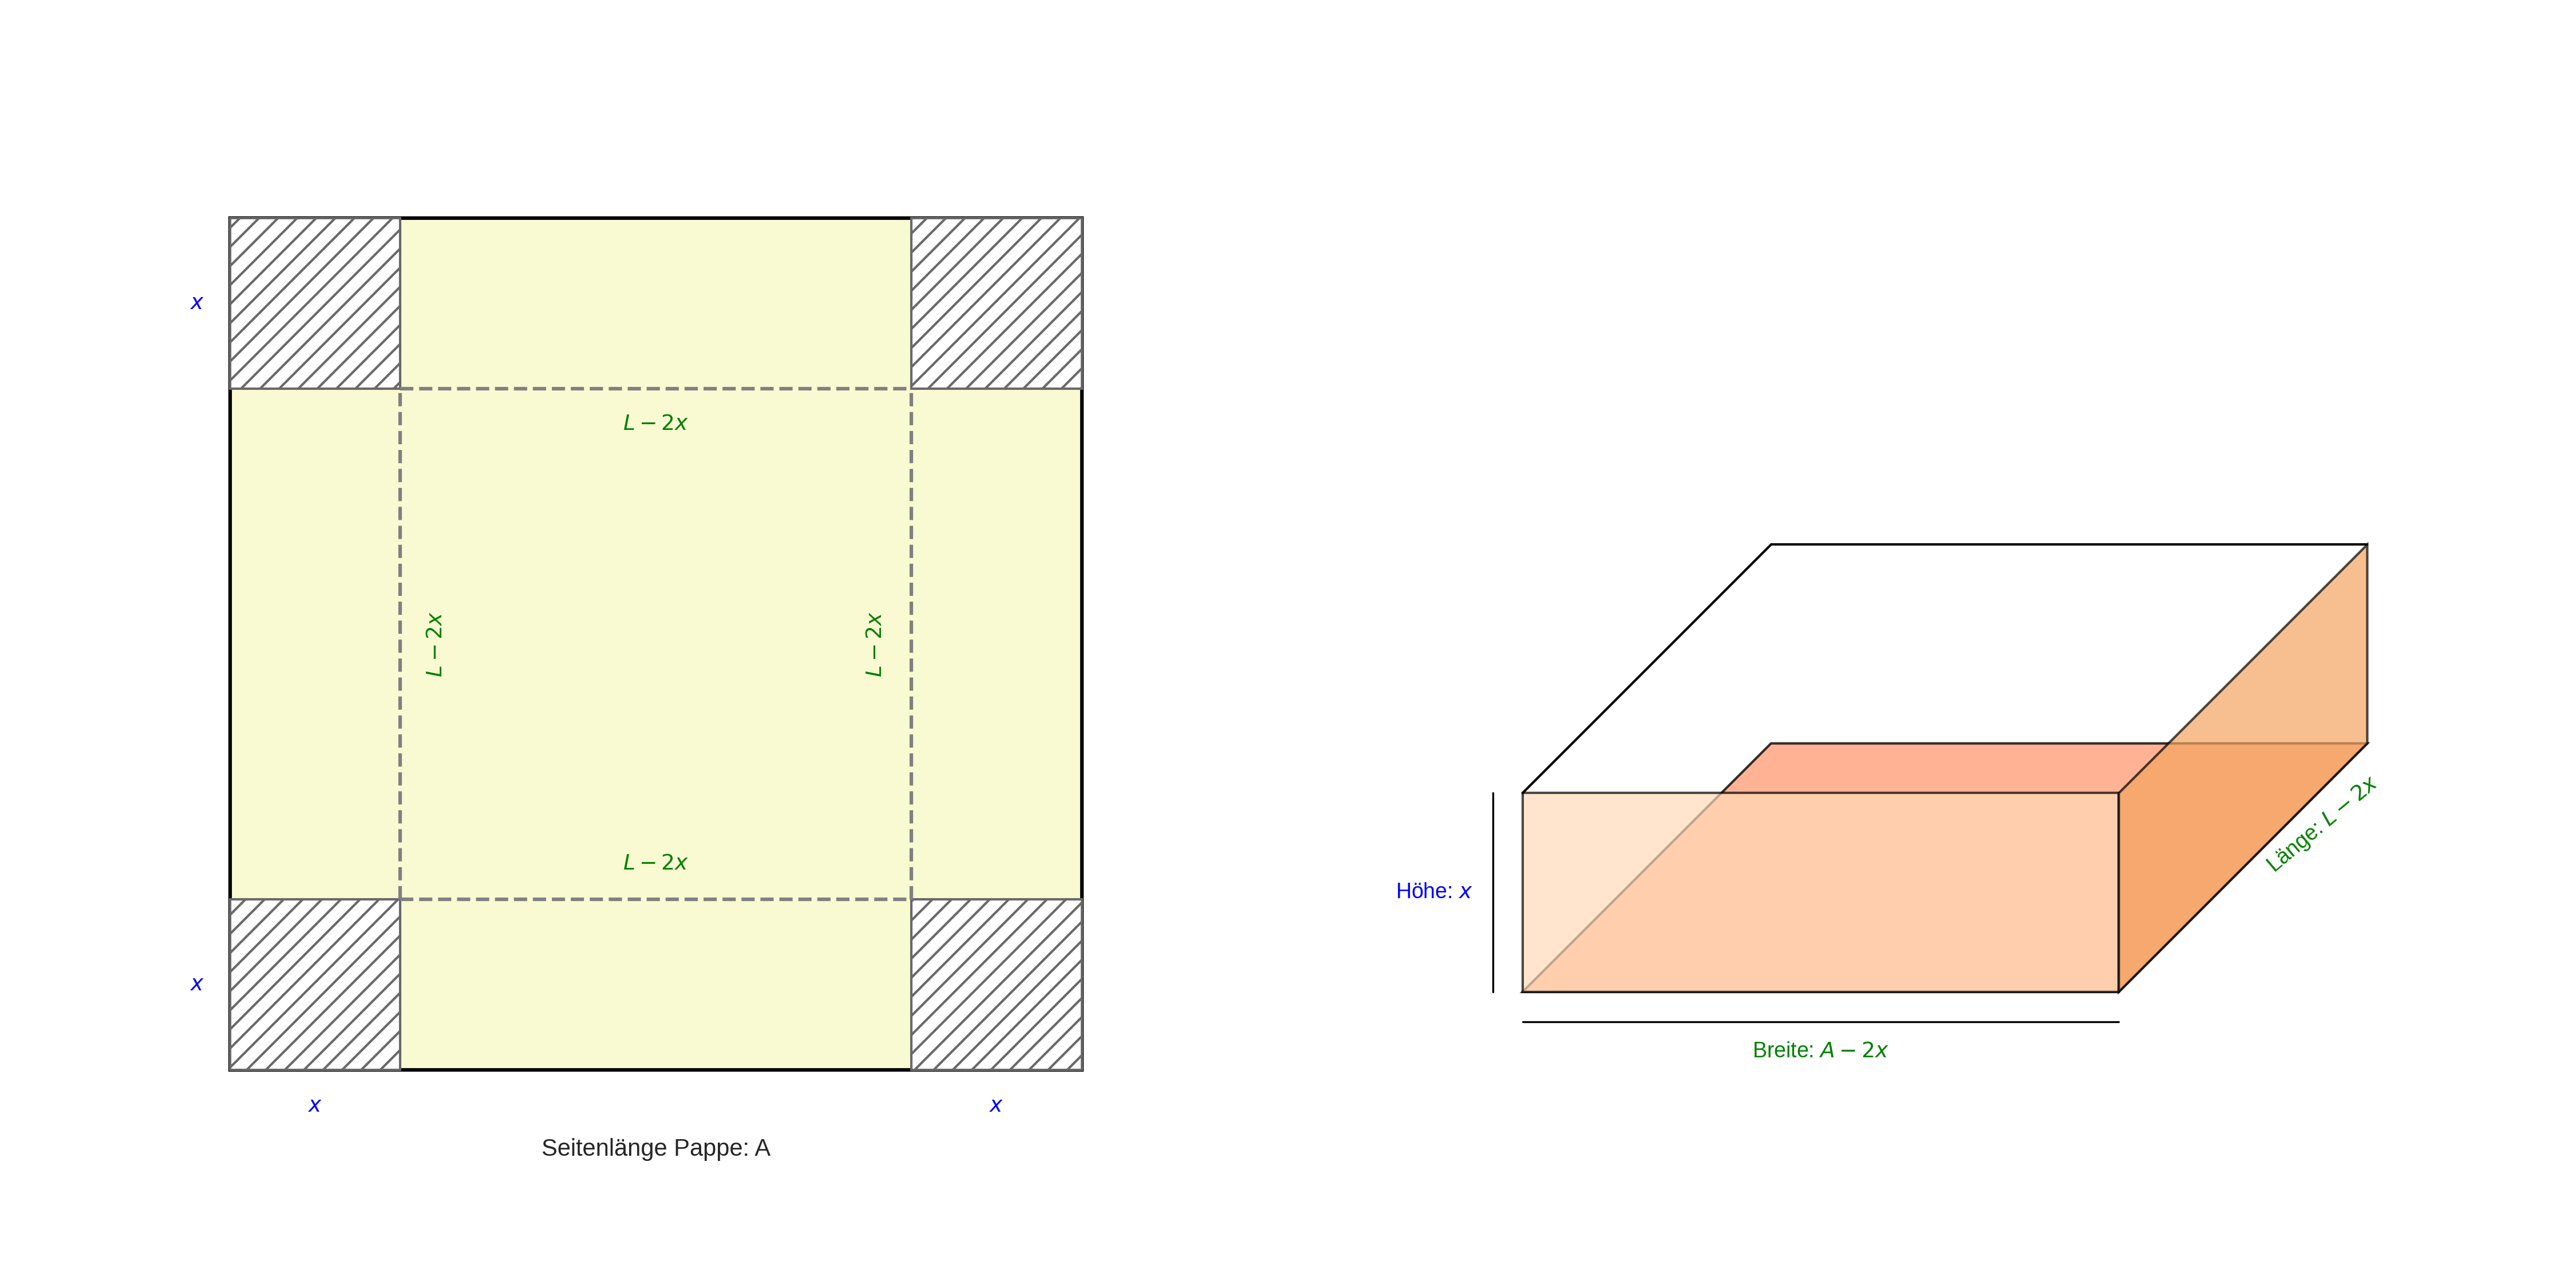
\includegraphics[width=0.9\textwidth]{grafiken/Optimierung_Schachtel.png}
    \captionof{figure}{Von der Pappe zur Schachtel}
    \label{fig:optimierung_schachtel}
\end{center}
\begin{enumerate}
    \item \textbf{Variable festlegen:} Sei $x$ die Seitenlänge der Quadrate, die an den Ecken ausgeschnitten werden.
    \item \textbf{Maße der Schachtel:} Drücke die Länge $l$, die Breite $b$ und die Höhe $h$ der entstehenden Schachtel in Abhängigkeit von $x$ aus. Bedenke, dass von jeder Seite der Pappe $2x$ weggeschnitten wird.
    \item \textbf{Definitionsbereich für $x$:} Welche Werte für $x$ sind in diesem Sachzusammenhang sinnvoll? (Die Seitenlängen müssen positiv sein, und man kann nicht mehr wegschneiden, als Pappe da ist).
    \item \textbf{Zielfunktion für das Volumen:} Stelle die Funktion $V(x)$ auf, die das Volumen der Schachtel in Abhängigkeit von $x$ beschreibt ($V = l \cdot b \cdot h$).
    \item \textbf{Extremwertsuche:}
        \begin{itemize}
            \item Bilde die erste Ableitung $V'(x)$.
            \item Setze $V'(x)=0$ und löse nach $x$, um die kritischen Stellen zu finden.
            \item Überprüfe mit der zweiten Ableitung $V''(x)$ (oder dem Vorzeichenwechselkriterium von $V'(x)$), ob an den kritischen Stellen ein Maximum oder Minimum vorliegt.
            \item Berücksichtige den Definitionsbereich von $x$: Liegen die gefundenen Extremstellen im sinnvollen Bereich?
        \end{itemize}
    \item \textbf{Antwort:} Gib die Seitenlänge $x$ der auszuschneidenden Quadrate an, für die das Volumen der Schachtel maximal wird, sowie das maximale Volumen selbst.
\end{enumerate}
\end{aufgabenumgebung}

\begin{aufgabenumgebung}{Rekonstruktion einer Polynomfunktion}
Eine ganzrationale Funktion dritten Grades $f(x) = ax^3 + bx^2 + cx + d$ hat die folgenden Eigenschaften:
\begin{itemize}
    \item Der Graph der Funktion geht durch den Ursprung $P(0|0)$.
    \item Der Ursprung ist gleichzeitig ein Wendepunkt der Funktion.
    \item Die Tangente im Wendepunkt (die Wendetangente) hat die Gleichung $y_W(x) = -3x$.
    \item Der Graph der Funktion hat eine Nullstelle bei $x_N = 1$.
\end{itemize}
Bestimme die Funktionsgleichung $f(x)$.

\begin{tippumgebung}{Bedingungen übersetzen}
Übersetze jede der gegebenen Eigenschaften in eine mathematische Gleichung für die Funktion $f(x)$ oder ihre Ableitungen $f'(x)$ und $f''(x)$:
\begin{itemize}
    \item 'Graph geht durch $P(x_0|y_0)$' $\implies f(x_0) = y_0$.
    \item 'Wendepunkt bei $x_W$' $\implies f''(x_W) = 0$.
    \item 'Tangentensteigung im Punkt $P(x_P|f(x_P))$ ist $m$' $\implies f'(x_P) = m$. Die Wendetangente gibt dir also die Steigung im Wendepunkt.
    \item 'Nullstelle bei $x_N$' $\implies f(x_N) = 0$.
\end{itemize}
Du erhältst ein lineares Gleichungssystem mit den Unbekannten $a, b, c, d$. Löse dieses System.
\end{tippumgebung}


\end{aufgabenumgebung}

\begin{infoboxumgebung}{Lineare Gleichungssysteme (LGS) lösen – Ein kurzer Überblick}
Wenn du die Bedingungen aus der Aufgabe oben in Gleichungen übersetzt, wirst du ein System von mehreren linearen Gleichungen mit mehreren Unbekannten ($a,b,c,d$) erhalten. So ein System nennt man \textbf{Lineares Gleichungssystem (LGS)}.
Zum Beispiel könnte ein einfaches LGS mit zwei Gleichungen und zwei Unbekannten $x,y$ so aussehen:
\begin{align*}
    I: \quad 2x + 3y &= 7 \\
    II: \quad x - y &= 1
\end{align*}
Es gibt verschiedene Methoden, solche Systeme zu lösen:
\begin{itemize}
    \item \textbf{Einsetzungsverfahren:} Eine Gleichung nach einer Variablen auflösen und diesen Term in die andere(n) Gleichung(en) einsetzen.
    \item \textbf{Gleichsetzungsverfahren:} Zwei Gleichungen nach derselben Variablen auflösen und die entstehenden Terme gleichsetzen.
    \item \textbf{Additions-/Subtraktionsverfahren:} Gleichungen (oder Vielfache davon) so addieren oder subtrahieren, dass eine Variable wegfällt.
\end{itemize}
Für größere Systeme mit mehr Variablen (wie hier mit $a,b,c,d$) werden diese Verfahren schnell unübersichtlich. Es gibt aber systematischere Methoden, wie das \textbf{Gaußsche Eliminationsverfahren} (oft auch mit Matrizen dargestellt), die in der Schule meist ausführlich behandelt werden.

\textbf{Für diese Aufgabe:}
Versuche, die vier Gleichungen, die du aus den Bedingungen erhältst, geschickt zu nutzen. Oft sind einige Gleichungen sehr einfach (z.B. wenn $f(0)=0$ direkt $d=0$ liefert). Setze bekannte Werte direkt in die anderen Gleichungen ein, um das System zu vereinfachen.

\textit{Hinweis zum Selbstlernen:} Das Lösen von LGS ist ein eigenes wichtiges Thema. Wenn du hier Schwierigkeiten hast, ist das nicht schlimm! Du kannst diesen Teil der Aufgabe überspringen oder dich auf das Aufstellen der Gleichungen konzentrieren. Das Lösen von LGS ist aber eine sehr nützliche Fähigkeit für viele Bereiche der Mathematik und darüber hinaus – es lohnt sich, das bei Gelegenheit zu üben! Diese Aufgabe ist eine gute Herausforderung, um dein mathematisches Denken zu schulen.
\end{infoboxumgebung}

\begin{aufgabenumgebung}{Bewegungsanalyse – Zwei Läufer auf der Bahn}
Zwei Läufer, A und B, bewegen sich auf einer geraden Bahn.
Läufer A startet zum Zeitpunkt $t=0\,$s am Punkt $s_A(0)=0\,$m. Seine Position (in Metern) zum Zeitpunkt $t$ (in Sekunden) wird durch die Funktion $s_A(t) = t^2$ beschrieben.
Läufer B startet gleichzeitig am Punkt $s_B(0)=10\,$m. Seine Position wird durch $s_B(t) = -0.5t^2 + 7t + 10$ beschrieben.
Wir betrachten das Zeitintervall $[0, 5]$ Sekunden.

\begin{enumerate}
    \item \textbf{Geschwindigkeiten:} Bestimme die Geschwindigkeitsfunktionen $v_A(t) = s_A'(t)$ und $v_B(t) = s_B'(t)$ der beiden Läufer.
    \item \textbf{Gleiche Geschwindigkeit:} Zu welchem Zeitpunkt $t$ haben beide Läufer die gleiche Geschwindigkeit? Wie groß ist diese Geschwindigkeit?
    \item \textbf{Gleiche Position:} Haben die Läufer jemals die gleiche Position im betrachteten Zeitintervall $[0,5]$? Wenn ja, zu welchem Zeitpunkt/welchen Zeitpunkten?
        \begin{tippumgebung}{Gleichung lösen}
        Um herauszufinden, wann sie die gleiche Position haben, musst du die Gleichung $s_A(t) = s_B(t)$ lösen. Das wird auf eine quadratische Gleichung führen.
        \end{tippumgebung}
    \item \textbf{Abstand der Läufer:}
        \begin{itemize}
            \item Stelle eine Funktion $d(t)$ auf, die den Abstand zwischen den beiden Läufern zum Zeitpunkt $t$ beschreibt. 
            \textit{Hinweis:} Überlege zuerst, welcher Läufer im Intervall $[0,5]$ vorne liegt, um das Betragszeichen bei der Differenz $d(t) = |s_B(t) - s_A(t)|$ auflösen zu können. Du hast in Teil c) untersucht, ob sie sich treffen.
            \item Zu welchem Zeitpunkt im Intervall $[0,5]$ ist der Abstand zwischen den Läufern minimal? Wie groß ist dieser minimale Abstand?
            \item Zu welchem Zeitpunkt im Intervall $[0,5]$ ist der Abstand zwischen den Läufern maximal? Wie groß ist dieser maximale Abstand?
            \begin{tippumgebung}{Extremwerte im Intervall}
            Um Extremwerte einer Funktion in einem abgeschlossenen Intervall $[t_1, t_2]$ zu finden, musst du die Funktionswerte an den kritischen Stellen (wo $d'(t)=0$) \textbf{und} an den Rändern des Intervalls ($t_1$ und $t_2$) untersuchen und vergleichen.
            \end{tippumgebung}
        \end{itemize}
\end{enumerate}
\end{aufgabenumgebung}

\begin{aufgabenumgebung}{Tangentenprobleme an einer kubischen Funktion}
Gegeben ist die Funktion $f(x) = x^3 - 3x$.
\begin{enumerate}
    \item \textbf{Parallele Tangenten:}
        \begin{itemize}
            \item Bestimme die Steigung der Geraden $g(x) = 9x - 5$.
            \item Gibt es Punkte auf dem Graphen von $f(x)$, an denen die Tangente parallel zur Geraden $g(x)$ ist? Wenn ja, bestimme die Koordinaten dieser Punkte.
            \item Gib die Gleichungen der Tangenten an den Graphen von $f(x)$ in diesen Punkten an.
        \end{itemize}
    \item \textbf{Tangente von einem externen Punkt:}
        Von welchem Punkt $P_y(0|y_P)$ auf der y-Achse aus kann man eine Tangente an den Graphen von $f(x)$ legen, die den Graphen an der Stelle $x_B=2$ berührt?
        \begin{tippumgebung}{Schrittweise Lösung}
        \begin{enumerate}
            \item Bestimme die y-Koordinate des Berührpunkts $B(2|f(2))$.
            \item Bestimme die Steigung $m_T$ der Tangente an den Graphen von $f(x)$ an der Stelle $x_B=2$.
            \item Stelle die Gleichung der Tangente $t_B(x)$ im Punkt $B$ auf.
            \item Der gesuchte Punkt $P_y(0|y_P)$ muss auf dieser Tangente $t_B(x)$ liegen. Setze $x=0$ in die Tangentengleichung ein, um $y_P$ zu finden.
        \end{enumerate}
        \end{tippumgebung}
\end{enumerate}
\end{aufgabenumgebung}
% Hier geht es dann weiter mit der Tippumgebung 'Struktur beim Ableiten komplexer Funktionen'
% und dem Abschluss des Kapitels.


% Hier geht es dann weiter mit der Tippumgebung 'Struktur beim Ableiten komplexer Funktionen'
% und dem Abschluss des Kapitels.
% Vorheriger Inhalt des Kapitels bis zur letzten aufgabenumgebung
% ... (siehe vorherige Canvas-Version, die mit der Aufgabe 'Tangentenprobleme an einer kubischen Funktion' endet) ...

% Dieser Block ersetzt den Kommentar:
% % Hier geht es dann weiter mit der Tippumgebung 'Struktur beim Ableiten komplexer Funktionen',
% % der Quotientenregel etc.



\begin{infoboxumgebung}{Ausblick auf weitere Ableitungsregeln und Funktionen}
Wir haben nun die wichtigsten Ableitungsregeln (Konstanten-, Potenz-, Faktor-, Summen-, Produkt-, Quotienten- und Kettenregel) kennengelernt. Mit diesem Werkzeugkasten kannst du schon eine riesige Bandbreite an Funktionen ableiten!

In den folgenden Kapiteln (oder in weiterführenden Kursen) wirst du lernen, wie man auch andere wichtige Funktionstypen ableitet, wie zum Beispiel:
\begin{itemize}
    \item \textbf{Exponentialfunktionen} (z.B. $f(x) = e^x$ oder $f(x) = 2^x$)
    \item \textbf{Logarithmusfunktionen} (z.B. $f(x) = \ln(x)$ oder $f(x) = \log_{10}(x)$)
    \item \textbf{Trigonometrische Funktionen} (z.B. $f(x) = \sin(x)$, $f(x) = \cos(x)$, $f(x) = \tan(x)$)
\end{itemize}
Die hier gelernten Regeln, insbesondere die Produkt-, Quotienten- und Kettenregel, werden auch für diese Funktionstypen von zentraler Bedeutung sein, wenn sie in Kombinationen auftreten (z.B. $f(x) = x \cdot e^x$ oder $f(x) = \sin(x^2)$).
Das Fundament, das du dir hier erarbeitet hast, ist also sehr wertvoll für alles, was noch kommt!
\end{infoboxumgebung}



\section*{Abschluss des Kapitels zur Differentialrechnung}

Herzlichen Glückwunsch! Du hast dich nun intensiv mit den Grundlagen der Differentialrechnung auseinandergesetzt. Von der intuitiven Idee der Tangentensteigung über die formale Definition der Ableitung bis hin zu den wichtigen Ableitungsregeln und ihrer Anwendung in Kurvendiskussionen und Optimierungsproblemen hast du einen weiten Weg zurückgelegt.

\begin{merksatzumgebung}[Was du mitnehmen solltest]{Kernkompetenzen dieses Kapitels}
\begin{itemize}
    \item Du verstehst die \textbf{Ableitung} als Maß für die momentane Veränderung einer Funktion und als Steigung ihrer Tangente.
    \item Du kannst die \textbf{grundlegenden Ableitungsregeln} (Konstanten-, Potenz-, Faktor-, Summen-, Produkt-, Quotienten- und Kettenregel) sicher anwenden, um die Ableitungsfunktionen verschiedener Funktionstypen zu bestimmen.
    \item Du kannst die \textbf{erste und zweite Ableitung} nutzen, um das Verhalten von Funktionen detailliert zu untersuchen: Monotonie, Art und Lage von Extrempunkten, Krümmungsverhalten und Wendepunkte.
    \item Du kannst das \textbf{Grenzwertverhalten} von Polynomen und einfachen gebrochen-rationalen Funktionen analysieren.
    \item Du bist in der Lage, eine \textbf{vollständige Kurvendiskussion} für Polynomfunktionen und einfache gebrochen-rationale Funktionen durchzuführen und deren Graphen zu skizzieren.
    \item Du hast erste Einblicke gewonnen, wie die Differentialrechnung zur Lösung von \textbf{Anwendungsproblemen} (z.B. Optimierung, Bewegungsanalyse) eingesetzt werden kann.
\end{itemize}
Diese Fähigkeiten sind nicht nur für die Mathematik selbst von großer Bedeutung, sondern bilden auch die Grundlage für viele Anwendungen in den Naturwissenschaften, der Technik und den Wirtschaftswissenschaften.
\end{merksatzumgebung}

\begin{infoboxumgebung}{Der Weg geht weiter...}
Die Differentialrechnung ist nur ein Teil der Analysis. Ein ebenso wichtiges und eng damit verbundenes Gebiet ist die \textbf{Integralrechnung}, mit der wir uns im nächsten Kapitel beschäftigen werden. Dort geht es darum, den umgekehrten Prozess zur Ableitung zu finden (das 'Aufleiten' oder Integrieren) und damit zum Beispiel Flächen unter Kurven oder Volumina von Rotationskörpern zu berechnen. Du wirst sehen, dass viele der hier gelernten Konzepte auch dort wieder eine Rolle spielen werden.

Bleib neugierig und übe fleißig weiter – die Welt der Mathematik hat noch viele spannende Entdeckungen für dich bereit!
\end{infoboxumgebung}

\begin{aufgabenumgebung}{Checkliste: Von kubischen Funktionen zu linearen Ableitungen}
Diese Aufgabe zeigt dir, wie dein Wissen über lineare Funktionen dir hilft, das Verhalten von Polynomen 3. Grades zu verstehen.
Betrachte die Funktion $f(x) = x^3 - 6x^2 + 10x - 3$.

\begin{enumerate}[label=(\alph*)]
    \item \textbf{Ableitungen bilden:} Berechne die erste Ableitung $f'(x)$ und die zweite Ableitung $f''(x)$ der Funktion $f(x)$.
    \item \textbf{Analyse der zweiten Ableitung:}
    \begin{itemize}
        \item Welchen Funktionstyp erkennst du in $f''(x)$? Gib die Steigung $m_{f''}$ und den y-Achsenabschnitt $c_{f''}$ dieser Funktion an.
        \item Berechne die Nullstelle $x_W$ von $f''(x)$. Welche besondere Bedeutung hat diese Stelle $x_W$ für den Graphen der ursprünglichen Funktion $f(x)$? (Erinnere dich an die Definition von Wendepunkten).
    \end{itemize}
    \item \textbf{Krümmungsverhalten von $f(x)$ bestimmen:}
    Nutze dein Wissen über lineare Funktionen, um das Vorzeichen von $f''(x)$ zu bestimmen:
    \begin{itemize}
        \item Für welche $x$-Werte ist $f''(x) > 0$? (Tipp: Wann sind die Werte einer steigenden/fallenden linearen Funktion positiv?)
        \item Für welche $x$-Werte ist $f''(x) < 0$?
        \item Welche Schlussfolgerungen ziehst du daraus für das Krümmungsverhalten (links- oder rechtsgekrümmt) des Graphen von $f(x)$? Gib die Intervalle an.
    \end{itemize}
    \item \textbf{Reflexion:} Erkläre in eigenen Worten, warum das Verständnis der Eigenschaften einer linearen Funktion (insbesondere ihrer Nullstelle und des Vorzeichenverlaufs in Abhängigkeit von der Steigung) nützlich ist, um das Krümmungsverhalten einer kubischen Funktion zu analysieren.
\end{enumerate}
\end{aufgabenumgebung}

\begin{aufgabenumgebung}{Checkliste: Von Polynomen 4. Grades zu quadratischen Ableitungen}
Diese Aufgabe zeigt dir, wie dein Wissen über quadratische Funktionen dir hilft, das Verhalten von Polynomen 4. Grades zu verstehen.
Betrachte die Funktion $g(x) = \frac{1}{4}x^4 - x^3 + x^2 + 1$.

\begin{enumerate}[label=(\alph*)]
    \item \textbf{Ableitungen bilden:} Berechne die erste Ableitung $g'(x)$ und die zweite Ableitung $g''(x)$ der Funktion $g(x)$.
    \item \textbf{Analyse der zweiten Ableitung:}
    \begin{itemize}
        \item Welchen Funktionstyp erkennst du in $g''(x)$? Gib die Parameter dieser Funktion an (z.B. Öffnungsfaktor, etc.). Ist der Graph von $g''(x)$ nach oben oder unten geöffnet?
        \item Berechne die Nullstellen $x_{W1}, x_{W2}$ von $g''(x)$ (falls vorhanden). Welche Bedeutung haben diese Stellen für den Graphen von $g(x)$?
    \end{itemize}
    \item \textbf{Krümmungsverhalten von $g(x)$ bestimmen:}
    Nutze dein Wissen über quadratische Funktionen, um das Vorzeichen von $g''(x)$ zu bestimmen:
    \begin{itemize}
        \item Skizziere (oder stelle dir vor) den Graphen von $g''(x)$ basierend auf Öffnungsrichtung und Nullstellen.
        \item Für welche $x$-Werte ist $g''(x) > 0$?
        \item Für welche $x$-Werte ist $g''(x) < 0$?
        \item Welche Schlussfolgerungen ziehst du daraus für das Krümmungsverhalten des Graphen von $g(x)$? Gib die Intervalle an. Wie viele Wendepunkte hat $g(x)$?
    \end{itemize}
    \item \textbf{Reflexion:} Erkläre, wie das Verständnis der Eigenschaften einer quadratischen Funktion (Öffnung, Nullstellen, Vorzeichenverlauf) hilft, das Krümmungsverhalten eines Polynoms 4. Grades zu analysieren.
\end{enumerate}
\end{aufgabenumgebung}

\begin{aufgabenumgebung}{Checkliste: Die maximale Steigung finden (Anwendung)}
Oft ist nicht nur interessant, wo eine Funktion ihren höchsten oder tiefsten Wert hat, sondern auch, wo sie am stärksten steigt oder fällt. Das führt uns zur Untersuchung der Ableitung selbst.
Ein Unternehmen stellt fest, dass seine Produktionskosten $K(x)$ (in Euro) bei der Herstellung von $x$ Einheiten eines Produkts durch die Funktion $K(x) = \frac{1}{3}x^3 - 10x^2 + 150x + 500$ für $x \in [0, 25]$ beschrieben werden können.
Die \textit{Grenzkosten} geben an, um wie viel die Kosten ungefähr steigen, wenn eine Einheit mehr produziert wird. Mathematisch sind die Grenzkosten die Ableitung der Kostenfunktion, also $K'(x)$.
Das Unternehmen möchte wissen, bei welcher Produktionsmenge $x$ die Grenzkosten $K'(x)$ \textbf{minimal} sind (d.h., wann die Kosten pro zusätzlich produzierter Einheit am geringsten ansteigen).

\begin{enumerate}[label=(\alph*)]
    \item \textbf{Grenzkostenfunktion bestimmen:} Bilde die erste Ableitung $K'(x)$ der Kostenfunktion $K(x)$. Diese Funktion $K'(x)$ beschreibt die Steigung der Kostenfunktion.
    \item \textbf{Ziel verstehen:} Wir suchen das Minimum der Funktion $K'(x)$. Wie findet man normalerweise Minima einer Funktion? (Tipp: Denke an die Ableitung der zu untersuchenden Funktion!)
    \item \textbf{Ableitung der Grenzkostenfunktion bilden:} Bilde die Ableitung von $K'(x)$, also die zweite Ableitung der ursprünglichen Kostenfunktion, $K''(x)$.
    \item \textbf{Kritische Stelle für $K'(x)$ finden:} Setze $K''(x) = 0$ und löse nach $x$. Dies ist die potenzielle Stelle $x_W$, an der die Grenzkosten $K'(x)$ minimal (oder maximal) sein könnten.
    \item \textbf{Art des Extremums von $K'(x)$ prüfen:} Überprüfe mit der nächsten Ableitung, also $K'''(x)$, ob bei $x_W$ tatsächlich ein Minimum für $K'(x)$ vorliegt. (Wenn $K'''(x_W) \neq 0$ und $K''(x_W)=0$, dann ist $x_W$ ein Wendepunkt von $K(x)$ und ein Extremum von $K'(x)$). Alternativ: Untersuche den Vorzeichenwechsel von $K''(x)$ bei $x_W$.
    \item \textbf{Antwort formulieren:} Bei welcher Produktionsmenge $x$ sind die Grenzkosten minimal? Wie hoch sind die minimalen Grenzkosten $K'(x_W)$?
    \item \textbf{Reflexion:} Was für ein besonderer Punkt ist $x_W$ für die ursprüngliche Kostenfunktion $K(x)$? Warum ist es plausibel, dass die Steigung einer Funktion (hier $K(x)$) an einem Wendepunkt maximal oder minimal wird?
\end{enumerate}
\end{aufgabenumgebung}

